
%  Beamer Style
\documentclass[xcolor={dvipsnames,rgb}]{beamer}

% \usepackage{enumitem}
%\includeonlyframes{current}
% \includeonlyframes{semantics,semantics2}

\usepackage{appendixnumberbeamer}

\usepackage{lmodern}
\usepackage[utf8]{inputenc}
\relax% Beamer Theme Customization...
    % \usetheme{default}
    \usetheme{Boadilla}
    % \ProcessOptionsBeamer
    % \useinnertheme[shadow]{rounded}
    \setbeamertemplate{blocks}[rounded][shadow=false]

    \setbeamertemplate{footline}
    {
      \leavevmode%
      \hbox{%
      \begin{beamercolorbox}[wd=.3\paperwidth,ht=2.25ex,dp=1ex,center]{author in head/foot}%
        \usebeamerfont{author in head/foot}\insertshortauthor
      \end{beamercolorbox}%
      \begin{beamercolorbox}[wd=.6\paperwidth,ht=2.25ex,dp=1ex,center]{title in head/foot}%
        \usebeamerfont{title in head/foot}\insertshorttitle
      \end{beamercolorbox}%
      \begin{beamercolorbox}[wd=.1\paperwidth,ht=2.25ex,dp=1ex,center]{date in head/foot}%
        \insertframenumber{} / \inserttotalframenumber\hspace*{1ex}
      \end{beamercolorbox}}%
      \vskip0pt%
    }

	\setbeamersize{description width=0.57cm}
	\usefonttheme[stillsansserifsmall]{serif}
		% \usefonttheme{structuresmallcapsserif}
	\usefonttheme[onlylarge]{structuresmallcapsserif}
		% \usefonttheme[onlymath]{serif}
		% \usefonttheme[onlysmall]{structurebold}
	\setbeamerfont{item}{series=\bfseries}
    \setbeamerfont{subsection in toc}{size=\small}
		% \setbeamerfont{section in toc}{size=\normalsize,series=\bfseries,shape=\upshape}
		\setbeamerfont{section in toc}{size=\normalsize}
	\setbeamerfont{block title}{series=\bfseries}
	% \setbeamerfont{title}{family=\rmfamily}

	\relax%%% color definitions %%...
		\colorlet{structurecolor}{RoyalPurple!50!black}
		\colorlet{alertcolor}{YellowOrange}
			% \colorlet{alertcolor}{structurecolor>wheel,1,3}
		\colorlet{benchcolor1}{Emerald!85!black}
			% \colorlet{benchcolor1}{structurecolor>wheel,2,3}
		\colorlet{benchcolor2}{YellowOrange!25!magenta}
	\usecolortheme[named=structurecolor]{structure}
		% \usecolortheme{beaver}
		% \setbeamercolor*{palette primary}{bg=color1, fg = green}
		% \setbeamercolor*{palette secondary}{bg=color2, fg = green}
		% \setbeamercolor*{palette tertiary}{bg=color3, fg = green}
		% \setbeamercolor*{palette quaternary}{bg=color4, fg = green}
		% \makeatletter
		% \definecolor{beamer@blendedblue}{rgb}{0.2,0.2,0.7}
		% \colorlet{beamer@blendedblue}{color2}
		% \makeatother
	\setbeamercolor{description item}{bg={structurecolor!20!white}}
	% \setbeamercolor{alerted text}{fg=alertcolor!85!red}
	\setbeamercolor{alerted text}{fg=alertcolor}
	\gdef\customnav{}
  % \setbeamertemplate{navigation symbols}{\customnav\insertframenavigationsymbol}
  \setbeamertemplate{navigation symbols}{\customnav~\insertsectionnavigationsymbol}
	\setbeamercolor{button}{fg=structurecolor,bg=structurecolor!15!white}
	\renewcommand\beamerreturnbutton[1]{{%
			\setbeamercolor{button}{fg=structurecolor!15!white,bg=black}%
			\beamerbutton{\insertreturnsymbol#1}%
		}}

  \makeatletter
  \newlength\beamerleftmargin
  \setlength\beamerleftmargin{\Gm@lmargin}
  %% stolen from:
  % https://tex.stackexchange.com/questions/34458/reference-overlay-numbers-with-names
  \DeclareRobustCommand*{\savepause}[1]{\only<1>{\immediate\write\@auxout{\string\pauseentry{\the\c@framenumber}{#1}{\the\c@beamerpauses}}}}
  \newcommand*{\usepause}[1]{\@ifundefined{pauses@\the\c@framenumber @#1}{1}{\@nameuse{pauses@\the\c@framenumber @#1}}}
  \newcommand*{\pauseentry}[3]{\global\@namedef{pauses@#1@#2}{#3}}
  \makeatother

  \newbool{precompiledfigs}% ...
	\setbool{precompiledfigs}{false}
		% the etoolbox way, which works with beamer.
	% \setbeamercovered{dynamic}

\relax %%%%%%%%  Beamer and slide-specific macros  %%%%%%%%%%%%%%%%%%%
	\newcommand<>{\hl}[2][alertcolor]{\begingroup%
		\setbeamercolor{alerted text}{fg=#1}\alert#3{#2}\endgroup}
	\colorlet{notationcolor}{structurecolor!30}
	\colorlet{notationalertedcolor}{structurecolor!20!alertcolor!40}
    \setbeamercolor{base notation}{fg=notationcolor}
    \setbeamercolor{alerted notation}{fg=notationalertedcolor}
	% \def\notation#1{\!\hl[notationcolor]{#1$\quad$}}
    \setbeamertemplate{alerted text begin}{
        % Set the notation color to alerted notation
        \setbeamercolor{notation}{use={alerted notation},%
            fg=alerted notation.fg,bg=alerted notation.bg}%
        %... and set the local structure to alerted text.
        \setbeamercolor{local structure}{use={alerted text},%
            fg=alerted text.fg,bg=alerted text.bg}}
    \setbeamertemplate{alerted text end}{%
        % probably no need to reset, because dying scope will reset the notation color.
        % \setbeamercolor{notation}{fg=base notation.fg, bg=base notation.bg}
    }
    % \setbeamercolor{notation}{parent={alerted text,normal text}}
	\newcommand{\notation}[1]{%
        {\usebeamercolor{notation}%
        \!\color{fg}#1$\quad$}}

	% \newcommand<>{\alertwith}[2]{\begingroup\only#3{\setbeamercolor{alerted text}{fg=#1}}#2\endgroup} % DOESN'T WORK THIS WAY
	\newenvironment{localfocusenv}{\only{\setbeamercolor{local structure}{fg=alertcolor}}}{}
	% \newenvironment<>{hidemeenv}{%
	% 	\only#1{\setbeamercolor{alerted text}{fg=black!60}}%
	% 	\begingroup\begin{alertenv}#1%
	% 	}{\end{alertenv}\endgroup}
	\newenvironment<>{hidemeenv}{%
        \begingroup\only#1{%
        %     \setbeamercolor{alerted text}{use={alerted text,background canvas},%
        %         fg=alerted text.fg!30!background canvas.bg}%
            \setbeamercolor{faded text}{%use={background canvas},%
                fg=normal text.fg!25!background canvas.bg}%
            \setbeamercolor{local structure}{use={faded text},fg=faded text.fg}%
            \setbeamercolor{notation}{use={base notation},fg=base notation.fg!40!background canvas.bg}
            \setbeamercolor{alerted notation}{fg=notationalertedcolor!30!background canvas.bg}
            \usebeamercolor[fg]{faded text}
        }}{\endgroup}
    \newenvironment<>{catblock}[1]{%
      \setbeamercolor{block title}{fg=white,bg=blue!95!black}
      \setbeamercolor{block body}{fg=white,bg=black}
      \begin{block}#2{#1}}{\end{block}}

	\newenvironment<>{tikzpicture||precompiled}[2][]{
			\ifbool{precompiledfigs}{\includegraphics[width=0.8\linewidth]{figure-pdfs/#2}
				}\begingroup\only#3\begingroup\begin{tikzpicture}[#1]
		}{\end{tikzpicture}\endgroup\endgroup}
	\newcommand<>{\extra}[2][]{%
		\only#3{%
			% \tikzmark{call point};%
			\tikzro \node[inner sep=0pt,outer sep=0pt] (call point) {};%
			\begin{tikzpicture}[overlay,remember picture]
				\node[anchor=north west, inner sep=0.8em,
				 			fill=alertcolor!30!structurecolor!30!white,
							draw=structurecolor!70!black, draw opacity=0.5,
							below=1em of call point, #1]{#2};
			\end{tikzpicture}%
		}}
	\newcommand{\tikzro}[1][]{\tikz[remember picture, overlay,#1]}
	\def\Set{\mathbf{Set}}
	% "light gray script script"
	\def\lgss{\color{gray!80}\scriptscriptstyle}%
	\makeatletter
	\newcommand{\shorteq}{%
	  \settowidth{\@tempdima}{-}% Width of hyphen
	  \resizebox{\@tempdima}{\height}{=}%
	}
	\makeatother
    %https://tex.stackexchange.com/questions/34921/how-to-overlap-images-in-a-beamer-slide
    \def\Put(#1,#2)#3{\leavevmode\makebox(0,0){\put(#1,#2){#3}}}

	% \newcommand{\tikzmark}[1][last mark]{\tikzro \node (#1){};}

%%%%%%%            Relevant part of PDG Preamble        %%%%%%%%%%%%%%%%
\usepackage{tikz}
	\usetikzlibrary{positioning,calc, arrows, shapes}

	\tikzset{AmpRep/.style={ampersand replacement=\&}}
	\tikzset{center base/.style={baseline={([yshift=-.8ex]current bounding box.center)}}}
	\tikzset{paperfig/.style={center base,scale=0.9, every node/.style={transform shape}}}

	\tikzset{dpadded/.style={rounded corners=2, inner sep=0.6em, draw, outer sep=0.2em, fill={black!50}, fill opacity=0.08, text opacity=1}}
	\tikzset{light pad/.style={outer sep=0.2em, inner sep=0.5em, draw=gray!50}}
	\tikzset{arr/.style={draw, ->, thick, shorten <=3pt, shorten >=3pt}}
	\tikzset{arr0/.style={draw, ->, thick, shorten <=0pt, shorten >=0pt}}
	\tikzset{arr1/.style={draw, ->, thick, shorten <=1pt, shorten >=1pt}}
	\tikzset{arr2/.style={draw, ->, thick, shorten <=2pt, shorten >=2pt}}

	\newcommand{\drawbb}%
		{\draw (current bounding box.south west) rectangle (current bounding box.north east);}
	\ifbool{precompiledfigs}{}{
		\usetikzlibrary{fit, decorations,shapes.geometric}
		\usetikzlibrary{tikzmark}
		\usetikzlibrary{backgrounds}
		\pgfdeclarelayer{foreground}
		\pgfsetlayers{background,main,foreground}

		\pgfdeclaredecoration{arrows}{draw}{
			\state{draw}[width=\pgfdecoratedinputsegmentlength]{%
				\path [every arrow subpath/.try] \pgfextra{%
					\pgfpathmoveto{\pgfpointdecoratedinputsegmentfirst}%
					\pgfpathlineto{\pgfpointdecoratedinputsegmentlast}%
				};
		}}

		% \tikzset{dpad0/.style={outer sep=0.05em, inner sep=0.3em, draw=gray!75, rounded corners=4, fill=black!08, fill opacity=1}}
		\tikzset{dpad0/.style={outer sep=0.05em, inner sep=0.2em, draw=gray!75, draw opacity=0.5, rounded corners=3, fill=black!18, fill opacity=0.4, text=black, text opacity=1}}

		\tikzset{dpad/.style args={#1}{every matrix/.append style={nodes={dpadded, #1}}}}
		\tikzset{is bn/.style={background rectangle/.style={fill=blue!35,opacity=0.3, rounded corners=5},show background rectangle}}
		% \usetikzlibrary{backgrounds}
		% \usetikzlibrary{patterns}
		\usetikzlibrary{cd}

		\tikzset{fgnode/.style={dpadded,inner sep=0.2em, circle,minimum width=2.3em},
				 factor/.style={light pad, fill=black, outer sep=0pt,draw=none}}


		\newcommand\cmergearr[5][]{
			\draw[arr, #1, -] (#2) -- (#5) -- (#3);
			\draw[arr, shorten <=0, #1] (#5) -- (#4);
			}
		\newcommand\mergearr[4][]{
			\coordinate (center-#2#3#4) at (barycentric cs:#2=1,#3=1,#4=1.2);
			\cmergearr[#1]{#2}{#3}{#4}{center-#2#3#4}
			}
		\newcommand\cunmergearr[5][]{
			\draw[arr, #1, -, shorten >=0] (#2) -- (#5);
			\draw[arr, shorten <=0, #1] (#5) -- (#3);
			\draw[arr, shorten <=0, #1] (#5) -- (#4);
			}
		\newcommand\unmergearr[4][]{
			\coordinate (center-#2#3#4) at (barycentric cs:#2=1.2,#3=1,#4=1);
			\cunmergearr[#1]{#2}{#3}{#4}{center-#2#3#4}
			}


		\usetikzlibrary{matrix}
		\tikzset{toprule/.style={%
		        execute at end cell={%
		            \draw [line cap=rect,#1]
		            (\tikzmatrixname-\the\pgfmatrixcurrentrow-\the\pgfmatrixcurrentcolumn.north west) -- (\tikzmatrixname-\the\pgfmatrixcurrentrow-\the\pgfmatrixcurrentcolumn.north east);%
		        }
		    },
		    bottomrule/.style={%
		        execute at end cell={%
		            \draw [line cap=rect,#1] (\tikzmatrixname-\the\pgfmatrixcurrentrow-\the\pgfmatrixcurrentcolumn.south west) -- (\tikzmatrixname-\the\pgfmatrixcurrentrow-\the\pgfmatrixcurrentcolumn.south east);%
		        }
		    },
		    leftrule/.style={%
		        execute at end cell={%
		            \draw [line cap=rect,#1] (\tikzmatrixname-\the\pgfmatrixcurrentrow-\the\pgfmatrixcurrentcolumn.north west) -- (\tikzmatrixname-\the\pgfmatrixcurrentrow-\the\pgfmatrixcurrentcolumn.south west);%
		        }
		    },
		    rightrule/.style={%
		        execute at end cell={%
		            \draw [line cap=rect,#1] (\tikzmatrixname-\the\pgfmatrixcurrentrow-\the\pgfmatrixcurrentcolumn.north east) -- (\tikzmatrixname-\the\pgfmatrixcurrentrow-\the\pgfmatrixcurrentcolumn.south east);%
		        }
		    },
		    table with head/.style={
			    matrix of nodes,
			    row sep=-\pgflinewidth,
			    column sep=-\pgflinewidth,
			    nodes={rectangle,minimum width=2.5em, outer sep=0pt},
			    row 1/.style={toprule=thick, bottomrule},
	  	    }
			}
		\usepackage{environ}
\usepackage{xstring}

% Wow this works I'm brilliant
\def\wrapwith#1[#2;#3]{
	\expandarg\IfSubStr{#1}{,}{
		\expandafter#2{\expandarg\StrBefore{#1}{,}}
		\expandarg\StrBehind{#1}{,}[\tmp]
		\xdef\tmp{\expandafter\unexpanded\expandafter{\tmp}}
		#3
		\wrapwith{\tmp}[#2;{#3}]
	}{ \expandafter#2{#1} }
}
\def\hwrapcells#1[#2]{\wrapwith#1[#2;&]}
\def\vwrapcells#1[#2]{\wrapwith#1[#2;\\]}
\NewEnviron{mymathenv}{$\BODY$}

\newcommand{\smalltext}[1]{\text{\footnotesize#1}}
\newsavebox{\idxmatsavebox}
\def\makeinvisibleidxstyle#1#2{\phantom{\hbox{#1#2}}}
\newenvironment{idxmatphant}[4][\color{gray}\smalltext]{%
	\def\idxstyle{#1}
	\def\colitems{#3}
	\def\rowitems{#2}
	\def\phantitems{#4}
	\begin{lrbox}{\idxmatsavebox}$%$\begin{mymathenv}
	\begin{matrix}  \begin{matrix} \hwrapcells{\colitems}[\idxstyle]  \end{matrix}
		% &\vphantom{\idxstyle\colitems}
		\\[-0.05em]
		\left[
		\begin{matrix}
			\hwrapcells{\phantitems}[\expandafter\makeinvisibleidxstyle\idxstyle]  \\[-1.2em]
	}{
		\end{matrix}\right]		&\hspace{-0.8em}\begin{matrix*}[l] \vwrapcells{\rowitems}[\idxstyle] \end{matrix*}\hspace{0.1em}%
	\end{matrix}%
	$%\end{mymathenv}
	\end{lrbox}%
	\raisebox{0.75em}{\usebox\idxmatsavebox}
%	\vspace{-0.5em}
}

\newenvironment{idxmat}[3][\color{gray}\smalltext]
	{\begingroup\idxmatphant[#1]{#2}{#3}{#3}}
	{\endidxmatphant\endgroup}

\newenvironment{sqidxmat}[2][\color{gray}\smalltext]
	{\begingroup\idxmat[#1]{#2}{#2}}
	{\endidxmat\endgroup}


%%%%%%%%%%%%
% better alignment for cases
\makeatletter
\renewenvironment{cases}[1][l]{\matrix@check\cases\env@cases{#1}}{\endarray\right.}
\def\env@cases#1{%
	\let\@ifnextchar\new@ifnextchar
	\left\lbrace\def\arraystretch{1.2}%
	\array{@{}#1@{\quad}l@{}}}
\makeatother

		\tikzset{onslide/.code args={<#1>#2}{%
		  \only<#1>{\pgfkeysalso{#2}} % \pgfkeysalso doesn't change the path
			}}
		}
		\newcommand{\TODO}[1][INCOMPLETE]{{\centering\Large\color{red}$\langle$~\texttt{#1}~$\rangle$\par}}

    % Tikz Externalization doesn't work with beamer with all of the animations...
    % \newif\ifexternalizefigures\externalizefigurestrue
    % \ifexternalizefigures
    % 	\usetikzlibrary{external}
    % 	\tikzexternalize[prefix=tikz/]  % activate!
    % 	\fi

\usepackage{booktabs,microtype}
\usepackage{mathtools, amsfonts, nicefrac, amssymb, bbm} % mathtools loads amsmath
\usepackage{array, booktabs}
% \usepackage{faktor} 
\usepackage[absolute,overlay]{textpos}
	\setlength{\TPHorizModule}{\textwidth}
	\setlength{\TPVertModule}{\textheight}
\usepackage{amsthm,thmtools}
	% \theoremstyle{plain}
	% \let\theorem\relax
	% \newtheorem{theorem}{Theorem}%[section]
	\newtheorem{coro}{Corollary}[theorem]
	\newtheorem{prop}[theorem]{Proposition}
	% \newtheorem{lemma}[theorem]{Lemma}
	% \newtheorem{fact}[theorem]{Fact}

	\theoremstyle{definition}
	\declaretheorem[name=Definition%,qed=$\square$,numberwithin=section
		]{defn}
	% \declaretheorem[name=Construction,qed=$\square$,sibling=defn]{constr}
	% \declaretheorem[qed=$\square$]{example}
	\theoremstyle{remark}
	\newtheorem*{remark}{Remark}
\relax % Macros (\relax is for folding)
	\let\Horig\H
	\let\H\relax
	\DeclareMathOperator{\H}{\mathrm{H}} %
	\DeclareMathOperator{\I}{\mathrm{I}} %
	\DeclareMathOperator*{\Ex}{\mathbb{E}} %
	\DeclareMathOperator*{\argmin}{arg\;min}
	\newcommand{\CI}{\mathrel{\perp\mspace{-10mu}\perp}} %
	\newcommand\mat[1]{\mathbf{#1}}
	\newcommand\Pa{\mathbf{Pa}}

	\DeclarePairedDelimiterX{\infdivx}[2]{(}{)}{#1\;\delimsize\|\;#2}
	\newcommand{\thickD}{I\mkern-8muD}
	\newcommand{\kldiv}{\thickD\infdivx}

	\newcommand{\tto}{\rightarrow\mathrel{\mspace{-15mu}}\rightarrow}

	\newcommand{\ssub}[1]{_{\!_{#1}\!}}
	\newcommand{\bp}[1][L]{\mat{p}\ssub{#1}}
	\newcommand{\V}{\mathcal V}
	\newcommand{\N}{\mathcal N}
	\newcommand{\Ed}{\mathcal E}

	\DeclareMathAlphabet{\mathdcal}{U}{dutchcal}{m}{n}
	\DeclareMathAlphabet{\mathbdcal}{U}{dutchcal}{b}{n}

	\newcommand{\dg}[1]{\mathbdcal{#1}}
	\newcommand{\pdgunit}{\mathrlap{\mathit 1} \mspace{2.3mu}\mathit 1}

	\newcommand{\IDef}[1]{\mathit{IDef}_{\!#1}}
	\newcommand\Inc{\mathit{Inc}}
	\newcommand{\PDGof}[1]{{\dg M}_{#1}}
	\newcommand{\UPDGof}[1]{{\dg N}_{#1}}
	\newcommand{\WFGof}[1]{\Psi_{{#1}}}
	\newcommand{\FGof}[1]{\Phi_{{#1}}}
	\newcommand{\Gr}{\mathcal G}
	\newcommand\VFE{\mathit{V\mkern-4mu F\mkern-4.5mu E}}

	%% Database Variables
	\newcommand{\D}{\mathbdcal D} % for a database
	\newcommand{\Idx}{\mathcal J}

	\newcommand{\datadist}[1]{\Pr\nolimits_{#1}}
    \newcommand\xsamp{{\underline{\mat x}}}
    \newcommand\xysamp{{\underline{\mat{xy}}}}

	\newcommand{\ed}[3]{%
		\mathchoice%
		{#2\overset{\smash{\mskip-5mu\raisebox{-3pt}{${#1}$}}}{\xrightarrow{\hphantom{\scriptstyle {#1}}}} #3} %display style
		{#2\overset{\smash{\mskip-5mu\raisebox{-3pt}{$\scriptstyle {#1}$}}}{\xrightarrow{\hphantom{\scriptstyle {#1}}}} #3}% text style
		{#2\overset{\smash{\mskip-5mu\raisebox{-3pt}{$\scriptscriptstyle {#1}$}}}{\xrightarrow{\hphantom{\scriptscriptstyle {#1}}}} #3} %script style
		{#2\overset{\smash{\mskip-5mu\raisebox{-3pt}{$\scriptscriptstyle {#1}$}}}{\xrightarrow{\hphantom{\scriptscriptstyle {#1}}}} #3}} %scriptscriptstyle

	% \DeclarePairedDelimiterX{\SD}[1]{\{}{\}}{\,\llap{\delimsize\{}#1\rlap{\delimsize\}}\,}
	%better version.
	% \DeclarePairedDelimiterX{\bbr}[1]{[}{]}
	% 	{\mspace{3mu}\mathllap{\delimsize[}#1\mathrlap{\delimsize]}\mspace{3mu}}
	% \DeclarePairedDelimiterX{\aar}[1]{\langle}{\rangle}
	% 	{\mspace{3mu}\mathllap{\delimsize\langle}#1\mathrlap{\delimsize\rangle}\mspace{3mu}}
	% \DeclarePairedDelimiterXPP{\aard}[1]{}{\langle}{\rangle}{_{\!_\downarrow}}
	% 	{\mspace{-3.5mu}\delimsize\langle#1\delimsize\rangle\mspace{-3.5mu}}
    \usepackage{scalerel}
    \newcommand{\nhphantom}[2]{\sbox0{\kern-2%
    		\nulldelimiterspace$\left.\delimsize#1\vphantom{#2}\right.$}\hspace{-.97\wd0}}
    		% \nulldelimiterspace$\left.\delimsize#1%
    		% \vrule depth\dp#2 height \ht#2 width0pt\right.$}\hspace{-.97\wd0}}
	\makeatletter
	\newsavebox{\abcmycontentbox}
	\newcommand\DeclareDoubleDelim[5]{
	    \DeclarePairedDelimiterXPP{#1}[1]%
			{% box must be saved in this pre code
				\sbox{\abcmycontentbox}{\ensuremath{##1}}%
			}{#2}{#5}{}%
		    %%% Correct spacing, but doesn't work with externalize.
			% {\nhphantom{#3}{##1}\hspace{1.2pt}\delimsize#3\mathopen{}##1\mathclose{}\delimsize#4\hspace{1.2pt}\nhphantom{#4}{##1}}
			%%% Fast, but wrong spacing.
			% {\nhphantom{#3}{~}\hspace{1.2pt}\delimsize#3\mathopen{}##1\mathclose{}\delimsize#4\hspace{1.2pt}\nhphantom{#4}{~}}
			%%% with savebox.
		    {%
				\nhphantom{#3}{\usebox\abcmycontentbox}%
				\hspace{1.2pt} \delimsize#3%
				\mathopen{}\usebox{\abcmycontentbox}\mathclose{}%
				\delimsize#4\hspace{1.2pt}%
				\nhphantom{#4}{\usebox\abcmycontentbox}%
			}%
    	}
    	\makeatother
    	\DeclareDoubleDelim
    		\SD\{\{\}\}
    	\DeclareDoubleDelim
    		\bbr[[]]
			\DeclareDoubleDelim
				\aarphantom{.{\phantom\langle}}{.{\phantom\langle}}{.{\phantom\rangle}}{.{\phantom\rangle}}
	% \DeclareDoubleDelim
	% 	\aar\langle\langle\rangle\rangle
	\makeatletter
	\newsavebox{\aar@content}
	\newcommand\aar{\@ifstar\aar@one@star\aar@plain}
	\newcommand\aar@one@star{\@ifstar\aar@resize{\aar@plain*}}
	\newcommand\aar@resize[1]{\sbox{\aar@content}{#1}\scaleleftright[3ex]
		{\Biggl\langle\!\!\kern0.3pt\!\!\Biggl\langle}{\usebox{\aar@content}}
		{\Biggr\rangle\!\!\kern0.3pt\!\!\Biggr\rangle}}
	\DeclareDoubleDelim
		\aar@plain\langle\langle\rangle\rangle
	\makeatother

%Information to be included in the title page:
% \title{Probabilsitic Dependency Graphs, and Inconsistency}
\title{Probabilistic Dependency Graphs and Inconsistency}
	% possibilities for third verb: mine, mobilize, mitigate, moderate
    \subtitle{How to model, measure, and mitigate internal conflict}
	\author[Oliver~Richardson]{Oliver Richardson}
	\institute[Cornell]{Cornell University\\Department of Computer Science}
	\date{September 2021}

\AtBeginSection[] { % Outline per section
  \begin{frame}<beamer>[noframenumbering]
    % \frametitle{Outline for section \thesection}
    \frametitle{Outline for Section \thesection}
		% \setlength\fboxsep{0pt}
		% \fbox{
    \begin{columns}[T]
				% \addtolength{\leftskip}{2cm}
        \column{0.45\textwidth}
				\begin{minipage}[t][0.84\textheight]{\linewidth}
				\raggedright
        \tableofcontents[currentsection,sections={<1-5,9-12>}]
				\end{minipage}

        \column{0.45\textwidth}
				\begin{minipage}[t][0.84\textheight]{\linewidth}
				\raggedright
        \tableofcontents[currentsection,sections={<6-8,13->}]
				\end{minipage}
    \end{columns}
		%}
  \end{frame}
	}

\begin{document}
\frame{\titlepage}

\section{Introduction}
\begin{frame}
    % First few sentences need to be about
    % (1) ease of use
    % (2)
    % Motivation:
    %  Suppose you're
    The standard way of modeling an agent with uncertainty:
		\pause
    \begin{itemize}[<+->]
            \setlength{\itemsep}{0pt}
            \setlength{\parskip}{0pt}
            \setlength{\parsep}{0pt}
        \item a probability distribution $p : \Delta W$ over worlds $W$,
        \item {\color{gray!80}(a utility function $u:\Omega \to \mathbb R$,
				% \item
				 	some actions $A$).}
    \end{itemize}
    \medskip

    \begin{center}
        \begin{tikzpicture}
					\onslide<2->{
            \node[dpadded, onslide=<3->{fill=blue!90}] (W) at (0,0) {$W$};
						\draw[arr2, <-] (W) -- node[above]{$p$} ++(-1.5, 0);  }
					%
					\begin{scope}[
							muted/.style={},
							onslide=<4->{
								draw=gray!40,%text opacity=0.4,
								muted/.style={text opacity=0.4, text=gray!80, fill opacity=0.08},
								dpadded/.append style={muted, fill=gray!25}}
						]
					\onslide<3->{
	            \node[dpadded] (O) at (2,0) {$\Omega$};
	            \node[dpadded] (U) at (3.8,0) {$U$};
							\draw[arr2, ->] (O) -- node[above, pos=0.35, muted]{$u$}  (U);
					% }	\onslide<4->{
							\node[dpadded] (A) at (0.8,1) {$A$};
							\mergearr[->] WAO
					 	}
					\end{scope}
        \end{tikzpicture}
    \end{center}

    % Interesting behavior arises from interactions with the environment or other agents, tricks to make computation tractable (independencies, approximation algorithms)
    % Addiction.
    \medskip
		\pause[\thebeamerpauses]
		\pause
		
    Such agents cannot have internal conflict;\\
    {\color{black}\hspace{1em}\small by construction, they have consistent beliefs and desires.}
\end{frame}

\begin{frame}
    % Rhetorical Question
		\frametitle{Why Inconsistency?}
		\begin{quotation}\small\it
				A man with a watch knows what time it is;\\
				a man with two watches is never sure.\\
				\hspace{1em}(Segal's Law)
			\end{quotation}
		\medskip
		Why \textbf{model} inconsistency?

		{%
				\setlength{\itemsep}{0pt}%
				\setlength{\parskip}{0pt}%
				\setlength{\parsep}{0pt}%
			\begin{itemize}[<+->]
					\item Sometimes people have inconsistent beliefs; %
						\begin{itemize}%%
						\item also want to understand the process of resolving it.
						\end{itemize}%
					% \item Internal conflict seems to drive important epistemic change.
				\end{itemize}%
		}

		\bigskip
		\pause[\thebeamerpauses]
		% Why \textbf{build a synthetic agent} that can be inconsistent%
		Why \textbf{construct} an agent that can be inconsistent%
			%{\small\color{gray}, if inconsistency bad}
			?

		% Why \textbf{entertain the possibility of being wrong}?
		\pause

		{%
			\setlength{\itemsep}{0pt}%
			\setlength{\parskip}{0pt}%
			\setlength{\parsep}{0pt}%
		\begin{itemize}[<+->]
				\setlength{\itemsep}{0pt}%
				\setlength{\parskip}{0pt}%
				\setlength{\parsep}{0pt}%
			% \item Why adopt beliefs without first cross-checking all knowledge?
			% \item Why entertain the possibility of being mistaken?
			\item Perfect consistency can be (needlessly) expensive.
				% Do you really do a full Bayesian update every time you learn something?
				% In effect, severely limits 
			\item Useful for identifying big problems.
			\begin{itemize}
				\item (assertions, check-sums, paradoxes)
			\end{itemize}
				% Guess an 
			% \item Why write assertions, that could disagree with the code?
			% \item Why imagine, when you could derive? 
			% \item Impossible to avoid if you aren't sure of logical relationships.
			% \item Internal conflict is a valuable process for introspection and driver of change.
			% \item Why consult multiple models, that can give inconsistent answers?
			% \item Less reliant on flawless design.
			% \item Epistemic modesty is a virtue.			
		\end{itemize}}
		\medskip

		\pause[\thebeamerpauses]
		% Internal conflict is valuable ,\\
		%% v1
		% Freedom from perfect consistency is valuable, \\
		% but demands that you also recognize and address internal conflict.
		%% v2
		% Internal conflict can let you better allocate computation \\
		% but demands the ability to recognize and adress it.
		%% v3 (incomplete)
		% Internal conflict is an important driver of change \\
		%% v4
		% Freedom from perfect consistency jrees up \textbf{a lot} of computation,
		% but demands the ability to recognize and adress internal conflict.
		%% v5
		Freedom from prefect consistency is valuable,
		but demands the ability to recognize and adress internal conflict.
		\smallskip
\end{frame}


\begin{frame}\frametitle{Yet Another Probabilistic Graphical Model}
	% We introduce \textit{probabilistic dependency graphs} (PDGs), a new class of graphical models
	% for representing uncertainty.
	%
	% \pause
	% \bigskip
	% {\centering\Large Why do we need another one?\par}
	%
	% \bigskip
	% \pause
	% \begin{itemize}[<+-|alert@+>]
	% 	\item To resolve inconsistency, we must first model it.
	% 	\item In doing so, we get much more \ldots
	% \end{itemize}

	% We introduce
	\textit{Probabilistic Dependency Graphs} (PDGs), \\
	a new class of graphical model
	% for representing uncertainty.
	designed to model inconsistent beliefs.

	\bigskip
	\hspace{1.5em}\pause
	In doing so, we get much more \ldots
	

	% \begin{itemize}[<+-|alert@+>]
	% 	% \item Designed to tolerate inconsistency, so we can model it.
	% 	\item Designed to model inconsistent beliefs.
	% 	\item In doing so, we get much more \ldots
	% \end{itemize}
\end{frame}

	\begin{frame} %%%%%%%%%%%        REVIEW OF BNS      %%%%%%%%%%%%%%%%
		\frametitle{Two aspects of Bayesian Networks (BNs)}
		\begin{description}
			\item<+->[{\color{benchcolor2!70!black}Qualitative} BN,~~$\Gr$]~\\
				an independence relation on variables
				\begin{itemize}\small
					\item {\color{gray} $X \CI_{\Gr} Y \mid \Pa(X)$, for all non-descendents $Y$ 	of $X$}
				\end{itemize}\medskip
			\item<+->[({\color{benchcolor1!80!black}Quantitative}) BN,~~$\mathcal B = (\Gr, \mat p)$]~\\
					a qualitative BN ($\Gr$) and a cpd
					$p_{\!_X}(X \mid \Pa(X))$ for each variable $X$.
					\vspace{-1.2em}
					%
					\begin{itemize} \small
						\item {\color{gray}Defines a joint distribution $\Pr_{\mathcal B}$
							% \hl[benchcolor2]<+>{
								with the independencies $\CI_\Gr$.
								% }
						}
					\end{itemize}
			\end{description}
		\vspace{2em}
		\begin{center}
			\begin{tikzpicture}[paperfig]
				\begin{scope}[every node/.style={dpadded, fill opacity=1,fill=black!08, circle, inner sep=2pt, minimum size=2em, draw=gray}]
					\node (PS) at (0,0) {$\mathit{PS}$};
					\node (SH) at (1.5, 0.6) {$\mathit{SH}$};
					\node (S) at (1.5, -0.6) {$\mathit{S}$};
					\node (C) at (3, 0) {$\mathit{C}$};
					\end{scope}
				\draw[->] (PS) to (S);
				\draw[->] (PS) to (SH);
				\draw[->] (SH) to (C);
				\draw[->] (S) to (C);
				\end{tikzpicture}
			\end{center}
		\end{frame}

\section{Modeling Examples}
	\subsection{What are Floomps?}
		\newlength{\bncolwidth}
		\begin{frame} %%%%%%%%%       GUN FLOOMP: BN vs PDG       %%%%%%%%%%
			%% 1 -- Just BN
			%% 2 -- add PDG.
			%% 3 -- List appears, arbitrary new info.
			%% 4 -- list highlighted, p appears both diagrams (dashed), green box.
			%% 5 -- inconsistent PDG?
			%% 6-8 -- variants of BN w / different info. Final point visible.
			\frametitle{Simple Example: Floomps and Guns}
			% \framesubtitle{The Legality of Floomps and Guns}
			\only<1-3>{
				{\centering	Grok thinks it likely (.95) that guns are illegal,\\
				but that floomps (local slang) are legal (.90).\par}
			}
			\pause
			\colorlet{heldout}{benchcolor1!80!black}

			% \only<2->{ % Headers "BN" and "PDG"
				\vspace{1.2em}
				\begin{columns}[c]
					\Large\color{structurecolor}
					\begin{column}{.45\textwidth}\centering% Add BN to diagram
						\only<4,5>{\color{structurecolor!20}}%
						\textbf{BN}\\[-1em]
						\rule{2.2cm}{0.95pt}\end{column}
					\only<3->{ % add PDG to diagram
						% \vrule
						\begin{column}{.5\textwidth}\centering%
							\only<6->{\color{structurecolor!20}}%
							\textbf{PDG}\\[-1em]
							\rule{2.7cm}{0.95pt}\end{column}
						}
					\end{columns}
				\vspace{0.0em}
				% }


			\begin{columns}[c] %% (both diagrams) ...
				\setlength{\bncolwidth}{0.45\textwidth}
				\only<6->{\setlength{\bncolwidth}{0.51\textwidth}}
				\begin{column}{\bncolwidth} % BN Diagram
					% \begin{block}{BN}
						\centering
						% \hspace{-2.5em}
						\begin{tikzpicture||precompiled}{fg-BN}[AmpRep, scale=0.9]
							\def\figtabledist{0.50}
							\def\fignodedist{0.8}
							\def\figtableheight{0.32}

							%% Time to unify the notation for cpds.
							% \matrix [table with head, column 1/.style={leftrule}, anchor=south east,
							% 	 column 2/.style={rightrule}, row 2/.style={bottomrule}] at (-\figtabledist,\figtableheight) {
							% 	\vphantom{$\overline fg$} $f$ \& \vphantom{$\overline fg$}$\overline f$\\
							% 	.9 \& .1\\
							% };
							% \matrix [table with head, column 1/.style={leftrule}, anchor=south west,
							% 	 column 2/.style={rightrule}, row 2/.style={bottomrule}] at (\figtabledist,\figtableheight) {
							% 	 \vphantom{$\overline fg$}$g$ \& \vphantom{$\overline fg$}$\overline g$\\
							% 	 .05 \& .95\\
							% };
							\node[% F's cpd ...
									anchor=south east]
							 	at (-\figtabledist,\figtableheight) {%
                                \color<6-8>{benchcolor1!70!black}
								\hspace{-1.2em}%
								\only<1-6,8>{\begin{idxmat} [\color{gray!60}\smalltext]
									{\!\!}{$f$,$\overline f$}
										.90 & .10 \\
									\end{idxmat}}%
								\only<7>{ \begin{idxmat}[\color{gray!60}\smalltext]
									{$g$,$\overline g$}{$f$,$\overline f$}
										.92 & .08 \\
										.08 & .92 \\
									\end{idxmat}\hspace{-1em}\;}%
								};
							\node[% G's cpd ...
									anchor=south west]
								at (\figtabledist,\figtableheight) {%
                                \color<6-8>{benchcolor1!70!black}
								\hspace{-1.2em}%
								\only<1-7>{\begin{idxmat}[\color{gray!60}\smalltext]
									{\!\!}{$g$,$\overline g$}
									.05 & .95 \\
									\end{idxmat}}%
								\only<8>{\begin{idxmat}[\color{gray!60}\smalltext]
									{$f$,$\overline f$}{$g$,$\overline g$}
										.92 & .08 \\
										.08 & .92 \\
									\end{idxmat}}%
								% \hspace{-0.5em}~%
								};
							\node[% F (floomp) ...
								dpadded, inner sep=0.5em, circle, fill=black!08, fill opacity=1]
								(floomp) at (-\fignodedist,0) {$F$};
							\node[% G (gun) ...
								dpadded, inner sep=0.5em, circle, fill=black!08, fill opacity=1]
								(gun) at (\fignodedist,0) {$G$};
							% \node (leftbounds) at (-3,0){};
							% \node (rightbounds) at (3,0){};

							\onslide<7,8>{ \draw[thick, ->, onslide=<8>{<-}, benchcolor2]
								(gun) -- node[below,align=center,font=\tiny]{must\\choose\\direction} (floomp); }

							% \only<6->{\node[align=left,% show which cpds are incorporated...
							% 		rounded corners=5, inner sep=0.5em,
							% 		fill=structurecolor!50!benchcolor1!10,
							% 		draw=structurecolor!50!benchcolor1!50] (incorporated)
							%  		at (0,-1.5)
							% 	{ \textit{BN Contents}:\\\Large
							% 		\hspace{1em}
							% 		\hl[benchcolor1]<6,8>{$\mu\ssub F$}
							% 		\hspace{1em}
							% 		\hl[benchcolor1]<6,7>{$\mu\ssub G$}
							% 		\hspace{1em}
							% 		\hl[benchcolor1]<8>{$p$}
							% 		\hspace{1em}
							% 		\hl[benchcolor1]<7>{$p'$}
							% 	};\node[below=1em of incorporated]{};}

							\only<4-6>{		\node[text=alertcolor] at (0,+0.8){$p$??};		}
							\only<4,5>{ \fill[white,opacity=0.8] (-3, -0.8) rectangle (3,1.8); }
							\useasboundingbox (-2.7, -0.8) rectangle (2.7,1.8);
							\end{tikzpicture||precompiled}
					% \end{block}
					\vspace{-0.8em}
					\end{column}
				\only<3,4>{{\color{gray}\vrule}}
				\begin{onlyenv}<3->\begin{column}{0.95\textwidth-\bncolwidth}
					% \only<6->{{~\hspace{-2em}~}}
					% \centering
					%%%%%%%%% PDG %%%%%%%%%%%%%
					\begin{tikzpicture||precompiled}{fg-PDG}[]
						\def\fignodedist{1.5}
						\node[% for  "1"  /  "true"  ...
							dpadded, fill=gray!50, draw=gray!70, inner sep=0.35em,
							outer sep=0.37em, densely dashed, text=gray, 
							text depth = 1em]
							(true)  at (0,1.3) {$\pdgunit$};
						\node[text=gray] at (0, 1.0){$\star$};
						
						\node[dpadded] (floomp) at (-\fignodedist, 0) {$F$};
						\node[dpadded] (gun) at (\fignodedist, 0) {$G$};

						\begin{pgfonlayer}{foreground}
							\draw[arr1,{onslide=<6,8>{benchcolor1!70!black}},
                                    {onslide=<7>{gray!50!white}}]
								(true.-165) -- %to[bend right=0]
									(floomp.60)
									node[pos=.5,{onslide=<6->{above left}}] (A)
										{\only<6->{$\mu\ssub F$}}
									;
							\draw[arr1,{onslide=<6,7>{benchcolor1!70!black}},
                                    {onslide=<8>{gray!50!white}}]
								(true.-15) -- %to[bend left=0]
									(gun.120)
									node[pos=.5,{onslide=<6->{above right}}] (B)
									 	{\only<6->{$\mu\ssub G$}}
									;
							\end{pgfonlayer}

						\node[, % CPT for F...
							above left=1.5em and 2.5em of A.center, anchor=center] {%
							\color<5>{alertcolor}
							\alt<6->{}{
								\hspace{-0.8em}%
								\begin{idxmat}
									[\color{gray!60}\color<5>{alertcolor!50}\smalltext]
									%[\color{black}\smalltext]
									{$\star$}{$f$, $\overline f$}
									.90 & .10 \\
								\end{idxmat}
								\hspace{-1em}~}
							};
						\node[, % CPT for G...
							above right=1.5em and 2.3em of B.center, anchor=center] {
							\color<5>{alertcolor}
							\alt<6->{}{
								\hspace{-0.8em}
								\begin{idxmat}
									[\color{gray!60}\color<5>{alertcolor!50}\smalltext]
									%[\color{black}\smalltext]
									{$\star$}{$g$, $\overline g$}
									.05 & .95 \\
								\end{idxmat}
								\hspace{-1em}~}
							};
						\only<4->{ % Show p & arrows, after initial diagrams...
							\begin{pgfonlayer}{foreground}
								\draw[arr,
										onslide=<4>{heldout, dashed},
                                        {onslide=<6,7>{gray!50!white}},
								 		{onslide=<8>{benchcolor1!70!black}},
										onslide=<5>{text=alertcolor} ]
								 	(floomp.-33) to[bend right=6] node[pos=0.65, fill=white, inner sep=2pt] (C) {$\smash{p}\vphantom{v}$} (gun.210);
								\draw[arr,
										onslide=<4>{heldout, dashed},
                                        {onslide=<6,8>{gray!50!white}},
										{onslide=<7>{benchcolor1!70!black}},
										onslide=<5>{text=alertcolor} ]
								 	(gun.190) to[bend left=5] node[pos=0.668, fill=white, inner sep=2pt] {$\smash{p'}\vphantom{v}$} (floomp.-10);
								\end{pgfonlayer}
							}
						\only<6->{ \fill[white,opacity=0.8] (-2.6, -1) rectangle (2.7,2); }%
						\useasboundingbox (-2.7, -0.8) rectangle (2.7,2.0);
						\end{tikzpicture||precompiled}
					% \vspace{-1em}
					\end{column}\end{onlyenv}
				\end{columns}
				% \only<-5>{\vspace{1em}}
			\begin{itemize} %% bullet points
				\item<3-| alert@3> The cpds of a PDG are attached to edges, not nodes.
				\item<4-| alert@4> PDGs can incorporate arbitrary new probabilistic information.
				\only<4>{ % New Information! The green block with cpts
					\vspace{0.7em} \color{black}
					\begin{exampleblock}{}
						% You come to believe that Floomps and Guns share legal status (92\%).
						{\small Grok learns that Floomps and Guns have the same legal status (92\%)}
						\vspace{-0.6em}
						$$ {\color{heldout}p(G \!\mid\! F)} =
							\begin{idxmat}[\color{gray!50}\smalltext]
									{$f$,$\overline f$}{$g$, $\overline g$}
								.92 & .08 \\ .08 & .92 \\
							\end{idxmat}
							~=~ {\left(\;{\color{heldout} p'(F \!\mid\! G)}\;\right)^{\textsf T}}$$
						\end{exampleblock}}
				\item<5-| alert@5> PDGs can be inconsistent\onslide<6->{,}
					\begin{itemize}
						\item<6- | alert@6> \textellipsis but BNs must resolve inconsistency first, \\
							{\small\color{gray} which may \hl<7-8>[benchcolor2]{break symmetry}
								and irrecoverably lose information.} %joe1
							\note{and so it may be better to wait to resolve it.}
						\end{itemize}
				\end{itemize}
			\end{frame} %------------%


	\subsection{Smoking BN Manipulations}
		\begin{frame}<-8>[label=smokingbnframe] %%%%%  SMOKING: BN vs PDG  %%%%%
			\frametitle{Bayesian Networks as PDGs}
			% \framesubtitle{Smoking and Cancer}
			\colorlet{heldout}{benchcolor1}
			\begin{center}
				\hfill
				\begin{tikzpicture||precompiled}[paperfig]{smoking-BN}
					\begin{scope} % BN Nodes...
						[every node/.style={dpadded, fill opacity=1,fill=black!08, circle, inner sep=2pt, minimum size=2em, draw=gray}]
						\node[onslide=<9->{opacity=0.2, text opacity=0.2}] (PS) at (0,0) {$\mathit{PS}$};
						\node (SH) at (1.5, -0.6) {$\mathit{SH}$};
						\node (S) at (1.5, 0.6) {$\mathit{S}$};
						\node (C) at (3, 0) {$\mathit{C}$};
						\end{scope}
					\draw[->,onslide=<9->{opacity=0.2}, onslide=<6>{benchcolor2,thick}] (PS) to (SH);
					\draw[->,onslide=<9->{opacity=0.2}] (PS) to (S);
					\draw[->] (S) to (C);
					\draw[->,onslide=<6>{benchcolor2,thick}] (SH) to (C);

					\only<9->{% Describe why restriction of BN is not a BN
						\node[below left=0.65 and 0.4 of PS,anchor=north west] (condBNtext)
						{\parbox{2.0in}{\small\raggedright\color{benchcolor1!60!alertcolor}
							Must now give distributions on $\mathit{SH}$ and $\mathit{S}$, or distinguish them as ``observed'' (a \emph{conditional} BN). %
							}};%
						}
					\end{tikzpicture||precompiled}%
				\hfill\pause\only<-9>{{\color<9->{gray!50}\vrule}}\hfill%
				\onslide<-8>{
				\begin{tikzpicture||precompiled}[paperfig]{smoking-PDG}
					\onslide<8->{ % Matt for restriction
						\fill[fill opacity=0.1, blue!80!black, draw, draw opacity=0.5] (2.73,1.35) rectangle (6.8, -1.35);}
					\alt<3->%
							{ \coordinate (1) at (0.1,0); }%
							{	\node[dpad0] (1) at (0,0) {$\pdgunit$}; }
					\node[dpadded] (PS) at (1.65,0) {$\mathit{PS}$};
					\node[dpadded, % (S) ...
					 	onslide=<8->{fill=black!.16, fill opacity=0.9},
						{onslide=<2>{yshift=0.5em}}]
						(S) at (3.2, 0.8) {$\mathit S$};
					\node[dpadded, % (SH)...
					 	onslide=<8->{fill=black!.16, fill opacity=0.9},
						{onslide=<2>{yshift=-0.5em}}]
						(SH) at (3.35, -0.8) {$\mathit{SH}$};
					\node[dpadded, % (C) ...
					 	onslide=<8->{fill=black!.16, fill opacity=0.9},
						{onslide=<2>{xshift=1.5em}}]
						(C) at (4.8,0) {$\mathit C$};

					\mergearr[draw opacity=0]{SH}{S}{C} % duplicated below; this one is to get coordinates right
					\onslide<4-5>{ % Draw cpts attached to each edge...
						% \node;
						\begin{scope}[thick,benchcolor1!80!black,dashed]
							\draw[] ($(1)!0.4!(PS)$) -- ++(0,0.85)
								node[above] {$p(\mathit{PS})$};
							\draw[] ($(PS)!0.5!(S)$) -- ++(-0.4,1.1)
								node[above] {$p(\mathit{S}\!\mid\!\mathit{PS})$};
							\draw[] ($(PS)!0.48!(SH)$) -- ++(-0.6,-0.75)
								node[below left] {$p(\mathit{SH}\!\mid\!\mathit{PS})$};
							\draw[] ($(center-SHSC)!0.11!(S)$) -- ++(0.6,0.75)
								node[above right] {$p(\mathit{C}\!\mid\!\mathit{S}, \mathit{SH})$};
							\end{scope}
						}

					\draw[arr1,  onslide=<5>{benchcolor1}] (1) -- (PS);
					\draw[arr2,  onslide=<5>{benchcolor1}] (PS) -- (S);
					\draw[arr2, onslide=<6>{benchcolor2}] (PS) -- (SH);
					\alt<2>{
							\node[dpad0] (centernode) at (center-SHSC) {\Tiny$\mathit{S} \times \mathit{SH}$};
							\draw[arr2,line width=0.6pt,->>] (centernode) -- (S);
							\draw[arr2,line width=0.6pt,->>] (centernode) -- (SH);
							\draw[arr2] (centernode) -- (C);
						}{
							\mergearr{SH}{S}{C} 
						}
					\only<6>{
						\draw[very thick,benchcolor2] (SH) -- (center-SHSC);
						\node[above=1pt of SH,benchcolor2]{?};
					}

					\onslide<7->{ % Add Tanning Beds & arrow...
						\node[dpadded,
							 	onslide=<7>{fill=benchcolor1!36, fill opacity=0.75,
								 	draw=benchcolor1!20!black, dashed},
								onslide=<8->{fill=black!.16, fill opacity=0.9}]
							(T) at (6.25,0) {$T$};
						\draw[arr1,onslide=<7>{dashed,draw=benchcolor1!60!black}] (T) -- (C);
						}
					\onslide<8>{ % Draw matt & label for restriction...
						\draw[very thick, |-|, color=blue!50!black,text=black] (2.7, 1.35) --coordinate(Q) (6.83,1.35);%
						\fill[white] (2.6, 1.36) rectangle (7.0,1.55);
						\node[above=0.05em of Q]{\small Restricted PDG};
						}
					\onslide<9-10>{ % Dim this picture for BN description...
						\fill[white, opacity=0.8] (current bounding box.south west) rectangle (current bounding box.north east); }
					\end{tikzpicture||precompiled}
				}
				\hfill
			\end{center}
			\vspace{1em}
			\only<10->{%
				\begin{tikzpicture}[overlay,yshift=3.5em,xshift=2.3in]
					%        \pgftransformshift{\pgfpointanchor{current page}{center}}
					\begin{scope}
							[every node/.style={dpadded, fill opacity=1,fill=benchcolor2!10, circle, inner sep=2pt, minimum size=2em, draw=gray!50!benchcolor2}]

						\node[] (A) at (1,0) {$A$};
						\node[right=0.5 of A, fill opacity=0.4, dashed] (B) {$B$};
						\node[right=0.5 of B] (C) {$C$};
					\end{scope}

					\draw[arr] (A) -- (B);
					\draw[arr] (B) -- (C);
					\node[anchor=south west] at (-0.5,0.4) {\parbox{2.5in}{\small\raggedright\color{benchcolor2}%
							In a qualitative BN: \emph{removing} data results in \emph{new} knowledge: $A \CI C$. \note{this is a larger set of distributions.} }};
				\end{tikzpicture}}%
			\pause\pause
			In contrast with BNs:
			\begin{itemize}%[<+-| alert@+>]
				\item<+-| alert@+-+(2)> edge composition has \emph{quantitative} meaning, since edges have cpds;%
					 \onslide<+>{}\onslide<+>{} % add two more frames
				\item<+-| alert@+> a variable can be the target of more than one cpd;
				\item<+-| alert@+> arbitrary restrictions of PDGs are still PDGs.\\
					{\small\begin{itemize}
						\item<+-| alert@+-+(1)> The analogue is false for BNs!
					\end{itemize}}
			\end{itemize}
			\gdef\customnav{\alt<2>{%
					\hyperlink{hypergraphextra}{\beamergotobutton{Hypergraphs!}}}{}}
			\end{frame}%------------%
			\gdef\customnav{}

	\subsection{Union and Restriction}
		\colorlet{colorsmoking}{blue!50!black}
		\colorlet{colororiginal}{benchcolor1!85!black}
		\begin{frame} %%%%%%%%%%         UNION OF PDGs         %%%%%%%%%%%%
			\frametitle{Combining PDGs}
			% \framesubtitle{Smoking and Cancer}
			\colorlet{heldout}{benchcolor1}
				\tikzset{hybrid/.style={postaction={draw,colorsmoking,dash pattern= on 5pt off 8pt,dash phase=6.5pt,thick},
					draw=colororiginal,dash pattern= on 5pt off 8pt,thick}}
			\begin{center}
					\begin{tikzpicture||precompiled}
							[paperfig, thick, colororiginal, fill opacity=0.2, text opacity=1, text=black]{grok-pre}
						\node[dpadded, fill=colororiginal] (C) at (0,0) {$\mathit C$};
						\node[dpadded, fill=colororiginal] (T) at (1.6,0){$\mathit T$};
						\node[dpadded, fill=colororiginal] (SL) at (.75,-1.4){$\mathit{SL}$};
                        \onslide<2->{
    						\draw[arr] (T) to[bend right] node[above]{$q$} (C); }
						\mergearr{C}{T}{SL}
						\end{tikzpicture||precompiled}
				\only<1-2>{
						\vspace{0.7em}
						\begin{exampleblock}{Grok wants to be supreme leader ($\mathit{SL}$).}

						\begin{itemize}[<+->]
							\item She notices that those who use tanning beds have more power, unless they get cancer \\[-0.4em]
							\item \textellipsis but mom says $q(C \mid T) = \begin{idxmat}
								{$t$,$\overline t$}{$c$,$\overline c$}
									.15 & .85 \\ .02 & .98
								\end{idxmat}$.\\[0.9em]
							% \item Grok worries getting cancer from a tanning bed will make $\mathit{SL}$ impossible.
						\end{itemize}
						\end{exampleblock}
					}
                \addtocounter{beamerpauses}{2}
				% \pause
                \onslide<+->{
    				% {\Large\!\!\!$\boldsymbol+$}
                    \!\!\scaleobj{2}{\sqcup}\!
    				% \hfill{\Large$+$}\hfill
    				\begin{tikzpicture||precompiled}[paperfig, text=black]{}
    					% \fill[fill opacity=0.1, blue!80!black, draw, draw opacity=0.5]
    					%  	(-2.07,1.35) rectangle (2.07, -1.35);
                        %
    					% 	\node[dpadded, fill=black!.16, fill opacity=0.9] (C) at (0,0) {$\mathit C$};
    					% 	\node[dpadded, fill=black!.16, fill opacity=0.9] (T) at (1.6,0){$\mathit T$};
    					% 	\node[dpadded, fill=black!.16, fill opacity=0.9] (S) at (-1.4, 0.8) {$\mathit S$};
    					% 	\node[dpadded, fill=black!.16, fill opacity=0.9] (SH) at (-1.45, -0.8) {$\mathit{SH}$};
                        \begin{scope}[thick, draw=colorsmoking, text=black, fill opacity=0.2, text opacity=1]
    						\node[dpadded, fill=colorsmoking] (C) at (0,0) {$\mathit C$};
    						\node[dpadded, fill=colorsmoking] (T) at (1.6,0){$\mathit T$};
    						\node[dpadded, fill=colorsmoking] (S) at (-1.4, 0.8) {$\mathit S$};
    						\node[dpadded, fill=colorsmoking] (SH) at (-1.45, -0.8) {$\mathit{SH}$};
        					\draw[arr1] (T) to node[above]{$p$} (C);
        					\mergearr{S}{SH}{C}
                        \end{scope}
					\end{tikzpicture||precompiled}
                    \hfill
                }
				% \hfill%
				\onslide<+->{
				% {\Large$\boldsymbol=$~}
                \\\vspace{-3em}\hfill
                    \!\!\scaleobj{2}{=}
				% \hfill%
				\begin{tikzpicture||precompiled}[paperfig, baseline={([yshift=-0.8ex]0,0)}]{grok-post}
					\begin{scope}[postaction={draw,colorsmoking,dash pattern= on 3pt off 5pt,dash phase=4pt,thick}]

						\node[dpadded,hybrid] (C) at (0,0) {$\mathit C$};
						\node[dpadded,hybrid] (T) at (2,0){$\mathit T$};
						\end{scope}

					\begin{scope}[thick, draw=colororiginal, text=black]
						\node[dpadded, fill=colororiginal!90!black, fill opacity=0.2] (SL) at (1,-1.5){$\it SL$};
						\draw[arr, onslide=<.(2)>{alertcolor}] (T) to[bend right] node[above]{$q$} (C);
						\mergearr{C}{T}{SL}
						\end{scope}

					\begin{scope}[thick, draw=colorsmoking, text=black, fill opacity=0.2]
						\node[dpadded,fill=colorsmoking] (S) at (-1.4, 0.8) {$S$};
						\node[dpadded,fill=colorsmoking] (SH) at (-1.45, -0.8) {$\mathit{SH}$};
						\draw[arr, onslide=<.(2)>{alertcolor}] (T) to node[fill=white, fill opacity=1,text opacity=1,inner sep=1pt]{$p$} (C);
						\mergearr{S}{SH}{C}
						\end{scope}
					\end{tikzpicture||precompiled}
                    }
				\end{center}
			\vspace{1em}
			\begin{itemize}[<+-|alert@+>]% [<+(1)-|alert@+(1)>]
				\item Arbitrary PDGs may be combined without loss of information
				\item They may have parallel edges %(e.g., $p,q$),
                    which directly conflict.
				\end{itemize}

			\end{frame}%------------%


\section{Syntax}
	\newlength{\pdgdefnwidth}
    % \subsection{Formal Definitions of PDGs}
	\begin{frame}[label=definition] %%%%%%%%%%%       Definition of a PDG          %%%%%%%%
		% \frametitle{Formal Definition}
		\colorlet{notationcolor}{structurecolor!40}
		% \setlength{\pdgdefnwidth}{\textwidth}
		% \begin{columns}[t]
		% \column{\pdgdefnwidth}
		\begin{defn}[Probabilistic Dependency Graph]\label{def:model}
			A PDG is a tuple $\dg M =
			(\N,\Ed,\V,\mat p, \alpha, \beta)$,\pause\ where
			\begin{description}%
				\item[$\N$]<+-> %\notation{$:\Set$}%
					is a finite set of nodes (variables)
					\begin{description}
						\item[$\V$]<+-> %\notation{$:\N \to \Set$}%
							gives a set $\V(X)$ of possible values for each $X$;%
							\extra<+>[anchor=north east, align=right]{
								$\displaystyle \V(\dg M) := \prod_{X \in \N} \V(X)\qquad$ is the set of
								 	possible \\[-0.75em] joint variable settings.		}
						\end{description}

				\item[$\Ed$]<+-> %\notation{$\subseteq \N \times \N \times \mathit{Label}~~~$}%
					is a set of labeled edges $\{ \ed LXY \}$, \hfill\hyperlink{hypergraphextra}{\beamergotobutton{(or hyper-edges)}}\\
					\pause[\thebeamerpauses]
					and associated to each $\ed LXY$, there is:

					\pause
					\begin{description}%[<+-| alert@+>]
						\item[$\bp$]<+-> %:\big(\!(X,Y,\ell)\in\!\Ed \big) \to
							%\notation{$:\V(X) \to \Delta\V(Y)$}%
							a cpd $\bp(Y \mid X)$;

						\item[$\alpha\ssub L$]<+(2)-> %\notation{$\in [0,\infty)$}%
						a confidence in the functional dependence $X \to Y$% $Y$ is a (noisy) function of $X$;
                        ;
						\item[$\beta\ssub L$]<+(-1)-> %\notation{$\in (0,\infty)$}%
							a confidence in the reliability of	$\bp$.
                % \extra<+(-1)>[anchor=north, align=center]{
								% 	write
								% 	``$p!$''
								% 	for the limit $(\beta_p \to \infty)$ \\[-0.25em]
                %   of high confidence in a cpd $p$.}
						\end{description}
				\end{description}
			\end{defn}
			% \column{\textwidth-\pdgdefnwidth}
			% \end{columns}

			% \begin{block}<+->{Equivalent Categorical Definition}
			% 	An unweighted PDG is a functor
			% 	${\color{benchcolor1}\langle \mat p, \V\rangle}\colon {\color{benchcolor2}\mathit{Paths}(\N, \Ed)} \to {\color{white}\mathbf{Mark}}$.
			%
		  %       So a PDG is a \emph{diagram} in ${\color{white}\mathbf{Mark}}$, in the usual mathematical sense.
			% 	\end{block}


		\end{frame}


% Details of PDG definition componnets & subsets + Category Theory


\section{Semantics}
\setbeamercolor{notation}{use={base notation}, fg=base notation.fg, bg=base notation.bg}
\begin{frame}<-2>[label=semantics]
    \frametitle{Semantics of PDGs}
		
		How to stitch cpds together?
    % \begin{description}[<+-|alert@+>]
    \begin{description}%[<+->]
        \item<+-|hideme@6-> [{$\SD{\dg M}$}] \notation{$\subseteq {\Delta \V(\dg M)}$} \\[0.15em]
            The set of joint distributions consistent with $\dg M$;
            \medskip

        \item<+-|alert@7> [{$\bbr{\dg M}_\gamma$}] \notation{$:{\Delta \V(\dg M)} \to \mathbb R$} \\[0.15em]
            A function {\small(parameterized by $\gamma > 0$)} that scores distributions by compatibility with $\dg M$;
            \medskip

        \item<+-|hideme@6->  [{$\bbr{\dg M}_\gamma^*$}] \notation{$\subseteq{\Delta \V(\dg M)}$} \\[0.25em]
            The distribution(s) most compatible with  $\dg M$\\
            (a singleton in many cases of interest);
            \medskip

        \item<+-> [{$\aar{\dg M}_\gamma$}] \notation{$: \mathbb R$} \\[0.15em]
            The best posssible compatibility of $\dg M$ with any distribution: the  \emph{inconsistency} of $\dg M$

				\item[{$\cdots$}]<+>~\\
					\hyperlink{sec:trace}{\beamergotobutton{trace semantics}}
    \end{description}
    % \pause
\end{frame}


%%%%%%%%%%%%%%%%%%%%   SCORING FUNCTION  %%%%%%%%%%%%%%%%
\relax % frame setup
	\colorlet{localcolor}{Lavender!80!black}
	\colorlet{globalcolor}{Sepia!80!orange}
	% \def\INCfst{2}
	\def\INCmotfst{2}
		% \def\INCmotlen{4}
		\def\INCmotlen{1}

	\edef\INCfst{\the\numexpr \INCmotfst + \INCmotlen \relax}
		% \def\INClen{5}
		\def\INClen{4}
		\edef\INClst{\the\numexpr\INCfst+\INClen-1\relax}
		\def\INCrange{\INCfst-\INClst}
		\def\INC+#1{\atslide{\INCfst+#1}}

	% \def\INCexfst{7}
	\edef\INCexfst{\the\numexpr \INClst + 1 \relax}
		\def\INCexlen{0}
		\edef\INCexlst{\the\numexpr\INCexfst+\INCexlen-1\relax}
		\def\INCexrange{\INCexfst-\INCexlst}
		\def\INCex+#1{\atslide{\INCexfst+#1}}

	\edef\IDEFmotfst{\the\numexpr \INCexlst + 1 \relax}
		\def\IDEFmotlen{3}
		% \def\IDEFmotlen{0}
		\def\IDEFmot+#1{\atslide{\IDEFmotfst+#1}}

	% \def\IDEFfst{12}
	\edef\IDEFfst{\the\numexpr \IDEFmotfst + \IDEFmotlen \relax}
		% \def\IDEFlen{3}
		\def\IDEFlen{4}
		\edef\IDEFlst{\the\numexpr\IDEFfst+\IDEFlen-1\relax}
		\def\IDEFrange{\IDEFfst-\IDEFlst}
		\def\IDEF+#1{\atslide{\IDEFfst+#1}}

	% \def\IDEFexfst{15}
	\edef\IDEFexfst{\the\numexpr \IDEFlst + 1 \relax}
		% \def\IDEFexlen{5}
		\def\IDEFexlen{0}
		\edef\IDEFexlst{\the\numexpr\IDEFexfst+\IDEFexlen-1\relax}
		\def\IDEFexrange{\IDEFexfst-\IDEFexlst}
		\def\IDEFex+#1{\atslide{\IDEFexfst+#1}}

	% \def\INCandIDEF{19}
	\edef\INCandIDEFfst{\the\numexpr\IDEFexlst + 1 \relax}
		\edef\INCandIDEF{\INCandIDEFfst-}
		\def\IIboth+#1{\atslide{\IDEFexlst + 1 + #1}}
		\edef\beforeINCandIDEF{-\the\numexpr\INCandIDEFfst - 1\relax}
		% \show\INCandIDEF
	\def\atslide#1{\the\numexpr#1\relax}
	\def\aitem@#1+#2{\item<\atslide{\csname#1fst\endcsname+#2}-|alert@\atslide{\csname#1fst\endcsname+#2}>}
	\def\halfblocks{\INCexrange,\IDEFexrange,\INCandIDEF}
\begin{frame}[t,label=semantics2] %%%
	\frametitle{The Scoring Function }
		\hypertarget<\IDEFexlst>{returntosemantics}{}
	\only<\IIboth+0->{ % this is actually at the end
		\begin{itemize}
			% \item<\IIboth+1-|alert@\IIboth+1> A BN strictly enforces the qualitative picture (large $\gamma$)
			% shifted from +2 to +1, when I substituted previous bullet
			\item<\IIboth+1-|alert@\IIboth+1> We are interested in the quantitative limit (small $\gamma$)
		\end{itemize}
		\bigskip
	}

	{\alt<\INCexrange,\IDEFexrange>{\vspace{-0.5em}\small}{\centering}\only<\INCandIDEF>{\centering}
		$\displaystyle%
			\bbr{\dg M}_\gamma(\mu) := \hl[alertcolor!30!benchcolor1!99!structurecolor]%
					<2-\INClst,\INCexrange,\INCandIDEF>{\Inc_{\dg M}(\mu)}
				+ \gamma%
				\extra<\IIboth+0>[below right=0.5em and -1 em of call point,
					inner sep=0.3em, font=\small, name=tp, draw=alertcolor, text=alertcolor!40!black,
					fill=alertcolor!10]{\small tradeoff parameter $\gamma \ge 0$}
				%
				\;\hl[alertcolor!30!benchcolor2!99!structurecolor]<\IDEFmotfst->{\IDef{\dg M}(\mu)}$\par}
			\only<\IIboth+0>{\tikzro{%
					\draw[alertcolor] ([yshift=-0.2em,xshift=-0.3em]call point.center) -- ([xshift=1.0em]tp.north west);}}

	{\medskip}
	\setlength\pdgdefnwidth{0.95\textwidth}
	% \only<\halfblocks>{\setlength\pdgdefnwidth{0.43\textwidth}}
	\only<\halfblocks>{\setlength\pdgdefnwidth{0.47\textwidth}}

	\only<\atslide{\INCmotfst}-\atslide{\INCfst-1}> {
		\smallskip
		{\centering\parbox{0.8\textwidth}{\raggedright
			\textbf{Intuition:}
			% beyond stating whether or not $\mu$ is consistent with $\dg M$, we
			% Measure the extent to which $\mu$ violates the constraints $\{\bp[]\}$ of $\dg M$.
			Measure $\mu$'s violation of $\dg M$'s cpds.
		}\par}

		\onslide<\atslide{\INCmotfst+1}-\atslide{\INCfst-1}>{
			{\color{structurecolor}\scshape{Motivating Examples}.}
			% \begin{center}
			\hfill
			$\dg M := \quad$
			\begin{tikzpicture}[paperfig]
				\node[dpadded] (1) {$\pdgunit$};
				\node[dpadded, right=1 of 1] (X) {$X$};
				\draw[arr1] (1) to[bend left=30] node[above] {$q$} (X);
				\draw[arr1] (1) to[bend right=30] node[below] {$p$} (X);
			\end{tikzpicture}
			\hfill~
			% \end{center}
			% \vspace{-1em}

			Suppose $p = [.4, .6]$.
		}
		\begin{itemize}
			% \aitem@{INCmot}+1 If $p = \begin{idxmat}{$\star$}{$x_1$,$x_2$} .4 & .6 \end{idxmat} = q$, then $\dg M$ is consistent, and compatible with the joint distribution $\mu(X) = p$.
			\aitem@{INCmot}+1 If $p = q$, then $\dg M$ is clearly consistent, and compatible with the joint distribution $\mu(X) = p = q$, so $\Inc_{\dg M}(p) = 0$.
					\medskip
			\aitem@{INCmot}+2 If
					% $p = \begin{idxmat}{$\star$}{$x_1$,$x_2$} .4 & .6 \end{idxmat}$
					% p = $[.4,.6]$
					% and
					% $q = \begin{idxmat}{$\star$}{$x_1$,$x_2$} .5 & .5 \end{idxmat}$,
					q = $[.5, .5]$
					then $\dg M$ is not consistent, but
					% $\mu = \begin{bmatrix}%{$\star$}{$x_1$,$x_2$}
					% 	.45 & .55 \end{bmatrix}$
					$\mu = [.45, .55]$
					matches better than
					% $\mu = \begin{bmatrix} .9 & .1 \end{bmatrix}$.
					$\mu= [.9, .1]$
					\medskip

			\aitem@{INCmot}+3 If
					% $p = \begin{bmatrix} .4 & .6 \end{bmatrix}$ and
					% $q = \begin{bmatrix} 0 & 1 \end{bmatrix}$,
					$q = [0,1]$,
					then $\dg M$ is much more inconsistent than before, even though $\SD{\dg M} = \emptyset$ in both cases.
		\end{itemize}
	}

	\begin{columns}[t]
		\only<\INCrange,\INCexrange,\INCandIDEF>{{ %%%%%%%%%% INC %%%%%%%%%%%%%%%
			\begin{column}{\pdgdefnwidth}
			\setbeamercolor{block title}{bg=benchcolor1!80!structurecolor!50}
			\setbeamercolor{block body}{bg=benchcolor1!80!structurecolor!20}
			\setbeamercovered{transparent=35}
			\only<\INCexrange>{\setbeamertemplate{blocks}[rounded][shadow=false]}
			\only<\INCexrange,\INCandIDEF>{\small}
			\begin{defn}[$\Inc$]<\INCrange,\INCandIDEF>\label{def:inc}
			The \emph{incompatibility} of
			\only<\INCrange>{a joint distribution }$\mu$ with $\dg M$\alt<\INCrange>{ is given by}{:}
			\def\fullnotate{\atslide{\INCfst+3}}
			\begin{align*}
				\alt<-\INC+2,\INCex+0->{ % The simpler, less clear notation
						\Inc_{\dg M}(\mu) :=&
							\sum_{\mathclap{\ed LXY}}\; \visible<\INC+1->{\alert<\INC+1>{\beta_L}} \;
							\tikzmark{relentD}
							\kldiv{ \mu_{Y|X} }{ \bp }
					}{  % The notation used in our paper
						\Inc_{\dg M }( \mu) :=&
							\sum_{\mathclap{\ed LXY}} \beta\ssub L \alert<\INC+3>{ \Ex_{x \sim \mu_{\!_X}} }
							\tikzmark{relentD}
							\kldiv[\Big]{ \mu \alert<\INC+3>{(Y \mid X \!=\! x)} }{\bp \alert<\INC+3>{(x)} }. }
					\alt<\INCex+0->{}{%
						\visible<\INC+4>{
							\\=& \Ex\nolimits_\mu \sum_{{\ed LXY}} \beta\ssub L
							 \Big(
								 % \I_{\bp} - \I_{\mu}
								 	\underbrace{~~\I_{\bp}~~}_{\parbox{0.9in}{\centering\footnotesize%
										code length,\\optimized for $\bp$\\to communicate\\$Y$ given $X$}} -
									\underbrace{~~\I_{\mu}~~}_{\parbox{0.9in}{\centering\footnotesize%
										code length,\\optimized for $\mu$\\to communicate\\$Y$ given $X$}}
								\Big)
							}}
				\end{align*}\vfill
			%
			\only<\INC+2-\INC+3>{
				\extra[name=Dexplain, below=1cm of pic cs:relentD, align=right,
							fill=benchcolor1!40!structurecolor!20!white]{%
							% is
							the
							relative entropy\\[-0.6em]%
						$\displaystyle\kldiv\mu\nu = \sum_{\mathclap{w \in \mathop{\mathrm{Supp}}\mu}} \mu(w) \log \frac{\mu(w)}{\nu(w)}\qquad$
						(KL Divergence) \\[-1.1em] from $\nu$ to $\mu$.
					}
				\tikzro \draw[thick,structurecolor!70!black,draw opacity=0.5]
					([xshift=0.5em,yshift=-0.2em]pic cs:relentD) -- ([xshift=0.5em]Dexplain.north); }
			% {\setbeamercovered{invisible}
			% 	\onslide<\INClst->{
			% 		The \emph{inconsistency} of $\dg M$ is \only<-\INClst>{the smallest possible incompatibility,}
			% 		\[ \Inc(\dg M) := \!\!\inf_{ \mu \in \Delta\V(\dg M)}\!\! \Inc_{\dg M}(\mu) . \]	 }}
			\end{defn}
			\end{column}
			}}
		\only<\INCexrange>{ %%% Inc Examples (omitted for AAAI + other talk, INC mot used instead)
			\column{\textwidth-\pdgdefnwidth}
			\vspace{-1em}
			{\centering\Large\color{structurecolor}\textsc{Examples}\par}
			\begin{center}
				\begin{tikzpicture}[throughlab/.style={fill=white, fill opacity=1,text opacity=1,inner sep=1pt}]
					\node[dpadded,thick] (C) at (0,0) {$\mathit C$};
					\node[dpadded,thick] (T) at (2,0){$\mathit T$};
					\draw[arr,draw=colororiginal,text=black] (T) to[bend right] node[throughlab]{$q$} (C);
					\draw[arr, draw=colorsmoking] (T) to node[throughlab]{$p$} (C);
					\end{tikzpicture}
				\end{center}

			\setlength{\leftmargini}{1em}
			\begin{itemize}
				\aitem@{INCex}+1 if $p = q$, then $\Inc(\dg M) = 0$.
				\aitem@{INCex}+2 if {\small $p =\begin{idxmat}%
							[\alt<\INCex+2>{\color{alertcolor!40}}{\color{gray!50}}\smalltext]
						{$t$,$\bar t$}{$c$} 0.4 \\ 0.1 \end{idxmat}$} and
					{\small $q = \begin{idxmat}%
							[\alt<\INCex+2>{\color{alertcolor!40}}{\color{gray!50}}\smalltext]
						{$t$,$\bar t$}{$c$} 0.9 \\ 0.1 \end{idxmat}$}, then \\[0.05em] still $\Inc(\dg M) = 0$
						(maybe nobody uses tanning beds).\vspace{0.4em}

				\aitem@{INCex}+3 {\small Not all inconsistencies are equally bad; \\
					\!\!$\Inc\!\left\{\!p \shorteq\!\! \begin{bmatrix} .55 \\ .12 \end{bmatrix}\!\!;
					q \shorteq\!\! \begin{bmatrix} .45 \\ .15 \end{bmatrix}\! \right\}\! < \!
					\Inc\! \left\{ \!p \shorteq\!\!\begin{bmatrix} .3 \\ .4 \end{bmatrix}\!\!;
					q \shorteq\!\! \begin{bmatrix} .9 \\ .1 \end{bmatrix}\! \right\}\!$}

				\end{itemize}
			}
		\only<\IDEFmotfst-\atslide{\IDEFfst-1}>{{
			\begin{column}{0.75\textwidth}

			\bigskip

			\textbf{Intuition:} each edge $\ed LXY$ indicates that $Y$ is determined (perhaps noisily) by $X$ alone.

			\bigskip
			\bigskip
			\bigskip

			\onslide<\IDEFmot+1->{
				So a $\mu$ with
				\tikzmark{beg-ce}%
					\hl[localcolor]<\IDEFmot+2->{uncertainty in $Y$ after $X$ is known}\tikzmark{end-ce}
				(beyond
				\tikzmark{beg-e}\hl[globalcolor]<\IDEFmot+2->{pure noise}\tikzmark{end-e})
				is qualitatively worse.

				\only<\IDEFmot+2>{
					\tikzro{ \draw[very thick,localcolor] ([yshift=0.8em]pic cs:beg-ce) -- %
						([yshift=1em]pic cs:beg-ce) --
							node[above,inner sep=2pt] {{\small\itshape measured by $\H(Y\mid X)$}}
						([yshift=1em]pic cs:end-ce) -- ([yshift=0.8em]pic cs:end-ce);}

					\tikzro{ \draw[very thick,globalcolor] ([yshift=-0.40em]pic cs:beg-e) --
							([yshift=-0.60em]pic cs:beg-e) -- node[below,inner sep=2pt] {$\H(\mu)$}
							([yshift=-0.60em]pic cs:end-e) -- ([yshift=-0.40em]pic cs:end-e);}
				}
			}

			\end{column}
			}}
		\only<\IDEFfst->{{ %%%%%%%%%% IDEF %%%%%%%%%%%%%
			\begin{column}{\pdgdefnwidth}
			\setbeamercolor{block title}{bg=benchcolor2!80!structurecolor!50}
			\setbeamercolor{block body}{bg=benchcolor2!80!structurecolor!20}
			\setbeamercovered{transparent=35}
			\only<\IDEFexrange>{\setbeamertemplate{blocks}[rounded][shadow=false]\small}
			\only<\IDEFexrange,\INCandIDEF>{\small}
			\begin{defn}[$\IDef{}$]<-\IDEFlst,\INCandIDEF>
				\alt<\halfblocks>
					{The $\dg M$-\emph{information deficiency} of $\mu$:
						% \vspace{2.0em}
						}
					{The \emph{information deficiency} of a distribution $\mu$ with respect to $\dg M$ is \vspace{4.2em}}
				%
				\def\idefdef{\sum_{\mathclap{\ed LXY}} \alt<\IDEFexfst->{\alpha\ssub L\!}{\alpha_L} \H_\mu(Y\!\mid\! X)}
				\[ \!\IDef{\dg M}(\mu) \alt<\IDEFexfst->{\!=\!}{:=}
					\alt<\IDEF+2->{{\color{localcolor}%
					 	\alt<\halfblocks>{\idefdef}{\overbrace{\idefdef}^{\tikzmark{lmark}}}}}{ \idefdef }
						-
					\alt<\IDEF+1->{{\color{globalcolor}%
						\alt<\halfblocks>{\H(\mu)}{\underbrace{\H(\mu)}_{\tikzmark{gmark}}}}}{ \H(\mu) } \alt<\halfblocks>{}{.}  \]
				\alt<\halfblocks>{}{ %IDef Overlays (a) and (b)
					\only<\IDEF+2->{% Overlay: (b) # bits to separately determine each target, knowing src...
						\extra[above left=0.6em and 1.2em of {pic cs:lmark},
							onslide=<\halfblocks>{inner sep=0.5em},
							anchor=south,align=center,
							name=idefseparate,
							fill=structurecolor!20!localcolor!40!white,
							text=localcolor!50!black]%
								{\alt<\halfblocks>{}{(b)} \# bits \alt<\halfblocks>{}{required }to separately
								determine\\ each target, knowing the source}
						\tikzro \draw[thick,draw=structurecolor!20!localcolor!70!black,draw opacity=0.6]
							(pic cs:lmark) -- ([xshift=1.2em]idefseparate.south);
						}
					\only<\IDEF+1->{% Overlay: (a) # bits to determine all variables...
						\extra[below right=1em and 2em of {pic cs:gmark},
							onslide=<\halfblocks>{below = 1em of pic cs:gmark, inner sep=0.5em},
							anchor=north east,name=entropy,
							fill=structurecolor!20!globalcolor!40!white,text=globalcolor!50!black]%
								{\alt<\halfblocks>{}{(a)} \# bits \alt<\halfblocks>{}{needed }to determine all \alt<\halfblocks>{vars}{variables}}
						\tikzro \draw[thick,draw=structurecolor!20!globalcolor!70!black,draw opacity=0.6]
							([yshift=0.5em]{pic cs:gmark}) -- ([xshift=-2em]{entropy.north east});
						}
					}
				
				% \alt<\halfblocks>{\vspace{1.8em}}{\vspace{3em}}
				\alt<\halfblocks>{\vspace{0em}}{\vspace{3em}}
			\end{defn}
			\end{column}}}
		\only<\IDEFexrange>{ %%%%%%%%%% IDEF EXAMPLES %%%%%%%%%%
			\column{\textwidth-\pdgdefnwidth}
			\vspace{-4em}

			{\centering\Large\color{structurecolor}\textsc{Examples}\par}

			\medskip
			\setlength{\leftmargini}{1.5em}
			\begin{itemize}
				% \setbeamercolor{alerted text}{fg=alertcolor!50!black}
				\aitem@{IDEFex}+0
					{$\dg M_0=\quad$\color<\IDEFex+0>{alertcolor!60!black}\begin{tikzpicture}[paperfig]
						\node[dpadded] (X) {$X$};
						\node[dpadded,right=0.8 of X] (Y) {$Y$};
					\end{tikzpicture}\hfill}~\\[0.3em]
					{\small\!$\IDef{\dg M_0}\!(\mu)\! =\!  - \H_\mu(X,Y)$}
					{\footnotesize\color{gray}\color<\IDEFex+0>{alertcolor!70!benchcolor2}%
					\\[-0.3em]~~(optimal $\mu$ maximizes entropy of $X,Y$)}~ \\[0.2em]
				\aitem@{IDEFex}+1
					{$\dg M_1=\quad$\color<\IDEFex+1>{alertcolor!60!black}\begin{tikzpicture}[paperfig]
						\node[dpadded] (X) {$X$};
						\node[dpadded,right=0.8 of X] (Y) {$Y$};
						\draw[arr2] (X) -- (Y);
					\end{tikzpicture}\hfill}~\\[0.3em]
					{\small\!$\IDef{\dg M_1}\!(\mu)\! =\! -\!\H_\mu(X)$}
					{\footnotesize\color{gray}\color<\IDEFex+1>{alertcolor!70!benchcolor2}\\[-0.3em]%
						~~(optimal $\mu$ maximizes entropy of $X$)}~  \\[0.2em]
				\aitem@{IDEFex}+2
					{$\dg M_2=\quad$\color<\IDEFex+2>{alertcolor!60!black}\begin{tikzpicture}[paperfig]
						\node[dpadded] (X) {$X$};
						\node[dpadded,right=0.8 of X] (Y) {$Y$};
						\draw[arr2] (X) to[bend left=15] (Y);
						\draw[arr2] (X) to[bend right=15] (Y);
					\end{tikzpicture}\hfill}~\\[0.3em]
					{\small\!$\IDef{\dg M_2}\!(\mu)\! =\!  - \H_\mu(X) + \H_\mu(Y\mid X)$}
					{\footnotesize\\\color{gray}\color<\IDEFex+2>{alertcolor!70!benchcolor2}%
						~~(optimal $\mu$ maximizes entropy for $X$, and\\[-0.4em]~~~~ makes $Y$ a function of $X$)}  \\[0.2em]
				\aitem@{IDEFex}+3
					{$\dg M_3=\quad$  \color<\IDEFex+3>{alertcolor!60!black}\begin{tikzpicture}[paperfig]
						\node[dpadded] (X) {$X$};
						\node[dpadded,right=0.8 of X] (Y) {$Y$};
						\draw[arr2] (X) to[bend left=10] (Y);
						\draw[arr2] (Y) to[bend left=10] (X);
					\end{tikzpicture}\hfill}~\\[0.3em]
					{\small\!$\IDef{\dg M_3}\!(\mu)\! =\!  - \I_\mu(X;Y)$}
					{\footnotesize\\[-0.3em]\color{gray} \color<\IDEFex+3>{alertcolor!70!benchcolor2}%
						(opt. $\mu$ makes $X,Y$ share information)}
			\end{itemize}

			\onslide<\IDEFex+4>%
				{\hyperlink{idefextra}{\beamergotobutton{Information Diagrams}}}
			}
		\end{columns}
		\alt<\IDEFlst>{
			\gdef\customnav{{\hyperlink{idefextra}{\beamergotobutton{Information Diagrams}}}}
		}{
			\gdef\customnav{}
		}
	\end{frame}



\begin{frame}
	\frametitle{The Optimal Distribution(s)}
	
	We have a scoring function $\bbr{\dg M}_\gamma : \Delta\V(\dg M) \to \mathbb R$.\\
	\pause
	Let $\bbr{\dg M}^*_\gamma$ be the set of best-scoring distributions.
	
	\pause
	
	\begin{prop}[{{\itshape\normalfont uniqueness for small $\gamma$, informal}}]
		As $\gamma\to0$, there is a unique optimal distribution, which we call $\bbr{\dg M}^*$.
	\end{prop}
	

	% \begin{prop}
	% 	\begin{itemize}
	% 		\item The second semantics extends the first, i.e,\\
	% 			$\SD{\dg M} \!= \big\{ \mu : \bbr{\dg M}_0(\mu) \!=\! 0 \big\}$.
	% 		\item If there there are distributions consistent
	% 			 		with $\dg M$, the best distribution is one of them. \\
	% 			$\bbr{\dg M}^* \in \bbr{\dg M}_0^*$, so if $\dg M$ is consistent,
	% 			then $\bbr{\dg M}^* \in \SD{\dg  M}$.
	%
	% 	\end{itemize}
	% \end{prop}
	\hypertarget{semantics-properties}{}
	\gdef\customnav{%
		\hyperlink{more-semantics-properties}{\beamergotobutton{Formal Statement + properties}}
		\hyperlink{semantics-relationships}{\beamergotobutton{Relationships Between Semantics}}
	}
\end{frame}
	\gdef\customnav{}




% \section{PDGs and other Graphical Models}
\section{Capturing other Graphical Models}
\subsection{Bayesian Networks}
	% \begin{frame}\frametitle{Construction}
	% \end{frame}

	\begin{frame}%%%%%%%%%          BN THEOREM
		\frametitle{Capturing Bayesian Networks}
		\onslide<2->{
      For a BN $\mathcal B$ with $N$ nodes and a vector $\beta \in \mathbb R^N$,
			let $\PDGof{\mathcal B, \beta}$ be the PDG
			corresponding to $\mathcal B$, with $\alpha=\mathbf 1$, and the given vector $\beta$ of confidences.
		}

    \begin{center}\only<.(1)>{\smash{
      \vspace{1em}
      \begin{tikzpicture}[{baseline=(current bounding box.north)}]
          \node[dpadded] (1) at (0,0) {$\pdgunit$};
          \node[dpadded] (PS) at (1.65,0) {$\mathit{PS}$};
          \node[dpadded] (S) at (3.2, 0.8) {$\mathit S$};
          \node[dpadded] (SH) at (3.35, -0.8) {$\mathit{SH}$};
          \node[dpadded] (C) at (4.8,0) {$\mathit C$};
          %
          \draw[arr1] (1) -- (PS);
          \draw[arr2] (PS) -- (S);
          \draw[arr2, onslide=<4>{benchcolor2}] (PS) -- (SH);
          \mergearr{SH}{S}{C}
        \end{tikzpicture}
			%
			}} \end{center}

    \vspace{-2em}
		\pause\pause
		\begin{theorem}[{{BNs are PDGs}}] \label{thm:bns-are-pdgs}
			% If $\mathcal B$ is a Bayesian network and $\Pr_{\mathcal B}$ is the distribution it specifies, then for all $\gamma > 0$ and all vectors $\beta$,
			If $\mathcal B$ is a BN and $\Pr_{\mathcal B}$ is the distribution it specifies, then for all $\gamma > 0$ and all vectors $\beta$,
			$$
				\bbr{\PDGof{\mathcal B, \beta}}_\gamma^* = \{ \Pr\nolimits_{\mathcal B}\},
				\quad\text{and thus}\quad
				\bbr{\PDGof{\mathcal B, \beta}}^* = \Pr\nolimits_{\mathcal B}.
			$$
			\end{theorem}

		\pause
		\begin{center}
		% \begin{minipage}{3.3cm}
		% 	\small
		% 	\setlength{\leftmargini}{0.2em}
		% 	\begin{itemize}
		% 		\item distributions consistent with $\dg M_{\mathcal B}$
		% 		\item these minimize $\Inc$
		% 	\end{itemize}
		% \end{minipage}
		\begin{tikzpicture}[remember picture,center base]
			\fill[benchcolor1,opacity=0.5] (0.1,0) -- (-1,1) -- (-2,0.7) -- (-2.5,-0.1) -- (-1.5, -0.5) -- cycle;
			\node[align=center] (sd) at (-1.3,0.2) {$\SD{\dg M}$};
			\fill[benchcolor2,opacity=0.5] (-0.1,0) -- (0.5,0.2)  -- (1, 1) -- (2, -0.5) -- cycle;
			\node[align=center] (ind) at (1,0.2) {$\CI_{\mathcal B}$};

			\node[left=0.9 of sd, inner sep=0.5pt, align=left, font=\small,
					text=benchcolor1!40!black] {
				space of distributions\\ consistent with $\dg M_{\mathcal B}$\\
				(which minimize $\Inc$)
			};
			\node[right=0.5 of ind, inner sep=0.5pt, align=right, font=\small,
				text=benchcolor2!40!black] {
				space of distributions\\ with independencies of $\mathcal B$\\
				(which can be shown \\ to minimize $\IDef{}$)
			};

			\node[fill=black, circle,inner sep=0.1em] (dot) at (0,0){};
			\node[below=0.5em of dot] (dotl) {$\Pr_{\mathcal B}$};
			\draw (dotl) -- (dot);
		\end{tikzpicture}
		% \begin{minipage}{3.2cm}
		% 	\setlength{\leftmargini}{0.5em}
		% 	\begin{itemize}
		% 		\item distributions with independencies of ${\cal B}$
		% 		\item can show that these minimize $\IDef{}$
		% 	\end{itemize}
		% \end{minipage}
		\end{center}

		% \vfill
		%
		% \begin{textpos}
		% \end{textpos}
		% \begin{textblock}{0.05}(0,1)
		% \stretch{}
		% \alt<2->{
		\only<.>{\hypertarget<.>{returntobns}{}
			\gdef\customnav{%
				{\hyperlink{sec:bnmaxent}{%
						\beamergotobutton{Corolary: BNs as Maximum Entropy Distributions}} }}%
			}
		% \end{textblock}
		\end{frame}
		\gdef\customnav{} % have to clear this.


\subsection{Factor Graphs}
\begin{frame}[label=factor-graph-intro] \frametitle{Factor Graphs}

	\vspace{-1.5em}
	\begin{center}
		\begin{tikzpicture}
			\begin{scope}[fgnode/.append style={onslide=<2>{draw=alertcolor,fill=alertcolor!50,fill opacity=0.3,text=alertcolor!50!black}}]
				\node [fgnode] (A) {$A$};
				\node [fgnode, right=1 of A] (B) {$B$};
				\node [fgnode, above=0.6 of B] (C) {$C$};
				\node [fgnode, right=1 of C] (D) {$D$};
				\node [fgnode, right=1 of B] (E) {$E$};
			\end{scope}

			\onslide<3->{
				\begin{scope}[factor/.append style={onslide=<3>{fill=alertcolor,
						draw=black, line width=2pt}}]
				\node[factor, left=0.5 of A, label={below:$\phi_1$}] (phi1) {};
					\draw[thick] (phi1) -- (A);

				\node[factor,label={below:$\phi_2$}] at ($(A)!.5!(B)$) (phi2) {};
					\draw[thick] (phi2) -- (A);
					\draw[thick] (phi2) -- (B);

				\node[factor,above=0.5 of phi2,label={above:$\phi_3$}] (phi3){};
					\draw[thick] (phi3) -- (A);
					\draw[thick] (phi3) -- (B);
					\draw[thick] (phi3) -- (C);

				\node[factor,label={above:$\phi_4$}] at ($(C)!.5!(D)$) (phi4) {};
					\draw[thick] (phi4) -- (C);
					\draw[thick] (phi4) -- (D);
				}
				\end{scope}
			\end{tikzpicture}
		\end{center}

	\begin{defn}
		A \only<7->{\alert<7>{weighted}} \emph{factor graph}
		\alt<-6>{$\Phi$}{$\Psi=(\Phi,\theta)$} is
		\pause
		a set of \alert<2>{variables $\mathcal X = \{X_i\}$},
		\pause\alt<-6>{and}{}
		\alert<3>{\emph{factors}\relax}
		 	$\{\phi_J\colon \V(X_J) \to \mathbb R_{\geq0}\}_{\alert<3>{J \in
		\mathcal J }}$,
		\only<7->{\alert<7>{and weights $(\theta_J)_{J \in \mathcal J}$}}
		with $X_J \subseteq \mathcal X$;
		\pause
		\alt<-6>{$\Phi$}{$\Psi$} defines a \alert<4>{distribution}
		\[ \alert<4>{{\Pr}_{\alt<-6>{\Phi}{\Psi}}(\vec x) :=}~\frac{1}{Z_{\Phi}}
		 	\prod_{J \in \cal J} \phi_J(\vec x_J)\only<7->{\alert<7>{^{\theta_J}}},
			\qquad\parbox{1.8in}{\raggedright where $Z_{\alt<-6>{\Phi}{\Psi}}$ is the\\normalization constant.}
			\]
		% \hfill 	where $Z_{\Phi}$ is the normalization constant.
		\end{defn}
		\pause

		%% :( :(
		% \alt<-6>{$\Phi$}{$\Psi$}
		% 	% defines a scoring function called ``variational free energy''
		% 	defines a standard scoring function
		% \[ \VFE_\Phi(\mu) := \Ex_{\mu} \Big[ - \sum_{J \in \mathcal J} \only<7->{\alert<7>{\theta_J}} \log {\phi_J(X_J)} \Big] - \H(\mu) \]
		\gdef\customnav{\hyperlink{semantics-thermo}{\beamergotobutton{\alt<-6>{$\Phi$}{$\Psi$}'s standard scoring function: ``variational free energy''}}}
	\end{frame}
%
%
% % Vague summary: factor graphs
% 	\begin{frame}
% 		\frametitle{PDGs and Factor Graphs}
%
%
% 		\begin{theorem}[{\it PDGs capture factor graphs}]
% 			We can naturally translate factor graphs and their exponential families%
% 				\note{(the natural notion of confidence in a factor graph)}%
% 				, into PDGs, in a way which preserves their semantics.
% 		\end{theorem}
%
% 		\bigskip
% 		Roughly speaking,
% 		\begin{itemize}
% 			\item a factor graph is a PDG in which qualitative and quantitative parameters are balanced $(\beta = \alpha\gamma)$.
%
% 			\item They have undesirable properties that do not occur in the quantitative limit.
% 		\end{itemize}
% 		% a factor graph is a PDG in which qualitative and quantitative parameters are balanced $(\beta = \alpha\gamma)$. They have undesirable properties that do not occur in the quantitative limit.
%
%
% 		See the paper for details!
%
% 		\end{frame}

% PDGs as factor graphs
\begin{frame} \frametitle{PDGs as Factor Graphs}
	\begin{center}
	\begin{tikzpicture||precompiled}[center base]{smoking-PDG}
		% \node[dpadded] (1) at (1.65,-1.1) {$\pdgunit$};
		\coordinate (1) at (1.65,-1.1);
		\node[dpadded] (PS) at (1.65,0.4) {$\mathit{PS}$};
		\node[dpadded] (S) at (3.2, 0.8) {$\mathit S$};
		\node[dpadded] (SH) at (3.35, -0.8) {$\mathit{SH}$};
		\node[dpadded] (C) at (4.8,0.4) {$\mathit C$};
		\node[dpadded] (T) at (4.8,-1.1) {$\mathit T$};

		\draw[arr1] (1) -- (PS);
		\draw[arr2] (PS) -- (S);
		\draw[arr2] (PS) -- (SH);
		\mergearr{SH}{S}{C}
		\draw[arr1] (T) -- (C);
		\end{tikzpicture||precompiled}
	~\pause{\Large$\rightsquigarrow$}~
	\begin{tikzpicture}[center base, xscale=1.2]
		\node[factor] (prior) at (1.65,-1) {};
		\node[factor] (center) at (3.75, 0.1){};

		\node[fgnode] (PS) at (1.65,0.5) {$\mathit{PS}$};
		\node[fgnode] (S) at (3.1, 0.8) {$\mathit S$};
		\node[fgnode] (SH) at (3.0, -0.8) {$\mathit{SH}$};
		\node[fgnode] (C) at (4.8,0.5) {$\mathit C$};

		\draw[thick] (prior) -- (PS);
		\draw[thick] (PS) --node[factor](pss){} (S);
		\draw[thick] (PS) --node[factor](pssh){} (SH);
		\draw[thick] (S) -- (center) (center) -- (SH) (C) -- (center);


		\node[fgnode] (T) at (4.8, -1.3) {$T$};
		\draw[thick] (T) -- node[factor]{}  (C);
		\end{tikzpicture}
		\end{center}


	\pause
	The cpds of a PDG are essentially factors. Are the semantics the same?
    \medskip
	% \pause
    % {\Large\raggedleft \alert<.(1)>{.}}

    \pause
	\begin{theorem}[{Yes, for $\gamma = 1$}]
		$\bbr{\dg N}_{1}^* = \Pr_{\FGof{\dg N}}\;$ for all unweighted
		PDGs $\dg N$.
	\end{theorem}
	\pause
	{\setbeamercolor{block body}{bg=structurecolor!50!white}
	 \setbeamercolor{block title}{bg=structurecolor!70!black,fg=white}
		\begin{theorem}[generalization to weighted factor graphs]
			Semantics match (for specific $\gamma$) if $\boldsymbol\beta \propto \boldsymbol\alpha$.
		\end{theorem}
	 }
	 \hypertarget<.>{returnto-pdg-is-wfg}{}

		\gdef\customnav{\alt<5>{\hyperlink{thm:pdg-is-wfg}%
			{\beamergotobutton{Precise Theorem Statement}}}{}}
	\end{frame}
	\gdef\customnav{}

% Why use PDGs over factor graphs
\begin{frame}\frametitle{An Important Difference between PDGs and Factor Graphs}
	\begin{center}
		$\dg M := $
		\begin{tikzpicture}[center base]
			\node[dpadded, inner sep=0.4em] (1){$\pdgunit$};
			\node[dpadded, inner sep=0.4em, below=1 of 1] (X) {$X$};
			\draw[arr] (1) to[bend left=30] node[right]{$p$} (X);
			\draw[arr] (1) to[bend right=30] node[left]{$q$} (X);
			\end{tikzpicture}
		$\qquad$ \vrule $\qquad$
		\begin{tikzpicture}[center base]
			\node[fgnode, below=1 of 1] (X){$X$};

			\node[factor, above left= 0.5 and 0.5 of X] (phi1) {};
			\node[factor, above right=0.5 and 0.5 of X] (phi2) {};

			\draw[thick] (phi1) -- (X);
			\draw[thick] (phi2) -- (X);
		\end{tikzpicture}$\quad=: \Phi$
	\end{center}
	\pause
	\medskip
	\begin{itemize}[<+-|alert@+>]
		\item If $p = q$, then $\bbr{\dg M}^* = p = q$\textellipsis
		\item \textellipsis but $\Pr_{\Phi} \propto p^2$
		% \item Individual factors have \emph{no probabilistic meaning}.
		% \item a factor graph can fail to normalize, in which case it has no global semantics either.
	\end{itemize}
	\end{frame}

% Factor graphs as PDGs
\begin{frame} \frametitle{Factor Graphs as PDGs}
	\begin{center}
		\begin{tikzpicture}[center base, xscale=1.3,
			fgnode/.append style={minimum width=2.4em, inner sep=0.2em}]
			\node[factor] (prior) at (1.65,-1) {};
			\node[factor] (center) at (3.75, 0.1){};

			\node[fgnode] (PS) at (1.65,0.5) {$\mathit{PS}$};
			\node[fgnode] (S) at (3.1, 0.8) {$\mathit S$};
			\node[fgnode] (SH) at (3.0, -0.8) {$\mathit{SH}$};
			\node[fgnode] (C) at (4.8,0.5) {$\mathit C$};

			\draw[thick] (prior) -- (PS);
			\draw[thick] (PS) --node[factor](pss){} (S);
			\draw[thick] (PS) --node[factor](pssh){} (SH);
			\draw[thick] (S) -- (center) (center) -- (SH) (C) -- (center);


			\node[fgnode] (T) at (4.8, -1.3) {$\mathit T$};
			\draw[thick] (T) -- node[factor]{}  (C);
			\end{tikzpicture}
		~{\Large$\rightsquigarrow$}~
		\pause
		% \begin{tikzpicture}[center base, xscale=1.5,
	  %       newnode/.style={rectangle, inner sep=5pt, fill=gray!30, rounded corners=3, thick,draw}]
		% 	\coordinate (prior) at (1.65,-1) ;
		% 	\coordinate (center) at (4.1, 0.25);
		% 
		% 	\node[dpadded] (PS) at (1.65,0.5) {$\mathit{PS}$};
		% 	\node[dpadded] (S) at (3.3, 0.8) {$\mathit S$};
		% 	\node[dpadded] (SH) at (3.3, -0.6) {$\mathit{SH}$};
		% 	\node[dpadded] (C) at (4.9,0.5) {$\mathit C$};
		% 
		% 	% \draw[arr, ->>, shorten <=0pt] (prior) -- (PS);
		% 	% \draw[arr, <<->>] (PS) --node[newnode](pss){} (S);
		% 	% \draw[arr, <<->>] (PS) --node[newnode](pssh){} (SH);
		% 	% \draw[arr, <<-, shorten >=0pt] (S) -- (center);
		% 	% \draw[arr, <<-, shorten >=0pt] (SH)-- (center);
		% 	% \draw[arr, <<-, shorten >=0pt] (C) -- (center);
		% 
		% 	% \node[dpadded, fill=blue] (1) at (2.7,-1.8) {$\pdgunit$};
		% 	\node[inner sep=1em, circle] (1) at (2.7,-1.8) {};
		% 
		% 	\coordinate (pss) at (barycentric cs:PS=1,S=1.2,1=0.1);
		% 	\coordinate (pssh) at (barycentric cs:PS=1.2,SH=1,1=0.2);
		% 	\coordinate (tc) at (barycentric cs:T=1.2,C=1,1=0.1);
		% 
		% 	\draw[blue!50,arr] (1) to[bend left=40] (PS);
		% 	\draw[blue!50,arr,shorten <=0pt] (pss) to[out=95, in=20] (PS);
		% 	\draw[blue!50,arr,shorten <=0pt] (pss) to[out=95, in=180] (S);
		% 
		% 	\draw[blue!50,arr,shorten <=0pt] (pssh) to[out=85, in=-20] (PS);
		% 	\draw[blue!50,arr,shorten <=0pt] (pssh) to[out=85, in=150] (SH);
		% 
		% 	% \draw[blue!50,arr, <->] (PS) -- (S);
		% 	% \draw[blue!50,arr, <->] (PS) --coordinate(pssh) (SH);
		% 	\draw[blue!50,arr, <-, shorten >=0pt] (S) to[out=0, in=90] (center);
		% 	\draw[blue!50,arr, <-, shorten >=0pt] (SH) to[out=45, in=90] (center);
		% 	\draw[blue!50,arr, <-, shorten >=0pt] (C) to[out=180, in=90] (center);
		% 
		% 
		% 	% \draw[blue!50, thick, shorten <=3pt] (1) -- (prior);
		% 	\draw[blue!50, thick, shorten <=3pt] (1) to[bend right=30] (center);
		% 	\draw[blue!50, thick, shorten <=3pt] (1) to[bend right = 5] (pss);
		% 	\draw[blue!50, thick, shorten <=3pt] (1) to[bend left = 10] (pssh);
		% 
		% 
		% 	\node[dpadded] (T) at (4.8, -1.7) {$T$};
		% 	\draw[blue!50,arr, shorten <=0pt] (tc) to[out=40,in=-110]  (C);
		% 	\draw[blue!50,arr, shorten <=0pt] (tc) to[out=30,in=115]  (T);
		% 
		% 	\draw[blue!50, thick, shorten <=3pt] (1.east) to[bend right = 15] (tc);
		% 	\end{tikzpicture}
		\begin{tikzpicture}[center base, xscale=1.5,
	        newnode/.style={rectangle, inner sep=5pt, fill=gray!30, rounded corners=3, thick,draw}]
			\coordinate (prior) at (1.65,-1) ;
			\coordinate (center) at (4.1, 0.25);
		
			\node[dpadded] (PS) at (1.65,0.5) {$\mathit{PS}$};
			\node[dpadded] (S) at (3.3, 0.8) {$\mathit S$};
			\node[dpadded] (SH) at (3.3, -0.6) {$\mathit{SH}$};
			\node[dpadded] (C) at (4.9,0.5) {$\mathit C$};
		
			% \draw[arr, ->>, shorten <=0pt] (prior) -- (PS);
			% \draw[arr, <<->>] (PS) --node[newnode](pss){} (S);
			% \draw[arr, <<->>] (PS) --node[newnode](pssh){} (SH);
			% \draw[arr, <<-, shorten >=0pt] (S) -- (center);
			% \draw[arr, <<-, shorten >=0pt] (SH)-- (center);
			% \draw[arr, <<-, shorten >=0pt] (C) -- (center);
		
			% \node[dpadded, fill=blue] (1) at (2.7,-1.8) {$\pdgunit$};
			\node[inner sep=1em, circle] (1) at (2.7,-1.8) {};
		
			\coordinate (pss) at (barycentric cs:PS=1,S=1.2,1=0.1);
			\coordinate (pssh) at (barycentric cs:PS=1.2,SH=1,1=0.2);
			\coordinate (tc) at (barycentric cs:T=1.2,C=1,1=0.1);
		
			\draw[blue!50,arr] (1) to[bend left=40] (PS);
			\draw[blue!50,arr,shorten <=0pt] (pss) to[out=95, in=20] (PS);
			\draw[blue!50,arr,shorten <=0pt] (pss) to[out=95, in=180] (S);
		
			\draw[blue!50,arr,shorten <=0pt] (pssh) to[out=85, in=-20] (PS);
			\draw[blue!50,arr,shorten <=0pt] (pssh) to[out=85, in=150] (SH);
		
			% \draw[blue!50,arr, <->] (PS) -- (S);
			% \draw[blue!50,arr, <->] (PS) --coordinate(pssh) (SH);
			\draw[blue!50,arr, <-, shorten >=0pt] (S) to[out=0, in=90] (center);
			\draw[blue!50,arr, <-, shorten >=0pt] (SH) to[out=45, in=90] (center);
			\draw[blue!50,arr, <-, shorten >=0pt] (C) to[out=180, in=90] (center);
		
		
			% \draw[blue!50, thick, shorten <=3pt] (1) -- (prior);
			\draw[blue!50, thick, shorten <=3pt] (1) to[bend right=30] (center);
			\draw[blue!50, thick, shorten <=3pt] (1) to[bend right = 5] (pss);
			\draw[blue!50, thick, shorten <=3pt] (1) to[bend left = 10] (pssh);
		
		
			\node[dpadded] (T) at (4.8, -1.7) {$T$};
			\draw[blue!50,arr, shorten <=0pt] (tc) to[out=40,in=-110]  (C);
			\draw[blue!50,arr, shorten <=0pt] (tc) to[out=30,in=115]  (T);
		
			\draw[blue!50, thick, shorten <=3pt] (1.east) to[bend right = 15] (tc);
			\end{tikzpicture}
		\end{center}
	\pause

	\begin{theorem}
		$\Pr_{\Phi} = \bbr{\UPDGof{\Phi}}_{1}^*\;$ for all factor graphs $\Phi$.
	\end{theorem}
	\pause
	{\setbeamercolor{block body}{bg=structurecolor!50!white}
	 \setbeamercolor{block title}{bg=structurecolor!70!black,fg=white}
	\begin{theorem}[]
		%%v1
		% If $\boldsymbol\beta = \gamma\boldsymbol\alpha $, then
		%%v2
		% $\Psi$ can be translated to a PDG $\dg M_{\Psi}$
		% where $\boldsymbol \beta = k \boldsymbol\alpha$, and \vspace{-0.5em}
		% \[ \Pr\nolimits_\Psi = \bbr{\dg M_{\Psi}}^*_k \]
		A simlar result holds for weighted factor graphs.
	\end{theorem}
	}
	\hypertarget<.>{returnto-wfg-is-pdg}{}
	% \pause
	% \begin{block}{}
	% 	Also: $\log Z_\Phi = \aar{{\dg N}_{\Phi}}_1$.
	% \end{block}
		\gdef\customnav{\hyperlink{thm:wfg-is-pdg}%
			{\beamergotobutton{Full Theorem}}}
	\end{frame}
	\gdef\customnav{}



\section{Inference}
\begin{frame}\frametitle{Inconsistency}
	Inconsistency: the optimal value of the scoring function.\\
	%No subscript means quantitative limit:
	% In the quantitative limit:
	% \[ \aar{\dg M} := \inf_{\mu} \Inc_{\dg M}(\mu) \]	
	\[ \aar{\dg M}_\gamma := \inf_{\mu}~ \bbr{\dg M}_\gamma (\mu) \]
	
	\bigskip
	\pause
	Nice properties for minimization:
	\begin{itemize}
		\item $\aar{\dg M}$ is strictly convex and smooth in cpds ~ {\small\color{gray}(on the interior)}
	\end{itemize}
	\end{frame}
\begin{frame}\frametitle{Inference via Inconsistency Reduction}
	% SAY OR TEXT
	% Usually: simple semantics, complicated inference. Here, semantics more complicated; inference = use the semantics.
	%
	% Identify the event $Y=y$ with the cpd  $\ed {{\mathbbm 1[Y\!=\!y]}}{\pdgunit} Y$.
	% Identify the event $Y\!\!=\!y$ with the cpd  $\ed {{\mathbbm 1[Y\!=y]}}{} Y$.
	% Identify the event $Y\!\!=\!y$ with the cpd  $\ed {{\delta_y}}{} Y$.
	% Identify the event $Y\!\!=\!y$ with the cpd ~~  $\ed {{\delta_y}}{\pdgunit} Y$.
	Identify the event $Y\!\!=\!y$ with the cpd ~~  $\ed {{\delta_y}}{} Y$.
	\medskip

	\pause
	\textbf{Conditioning as inconsistency resolution.}\\
		% To condition on $Y\!=\!y$  in $\dg M$,
		% simply add
		%  $\ed {\delta_y}{\pdgunit} Y$  to get ${\dg M}_{Y\!=y}$.
		% Then the optimal distribution $\bbr{{\dg M}_{Y\!=y}}^*$ is the same as conditioning the optimal distribution $\bbr{\dg M}^*$ for $\dg M$ on $Y\!=\!y$. That is,
		% \[ \bbr{{\dg M}_{Y\!=y}}^* = \bbr{\dg M}^* \mid (Y\!=\!y).\]
		To condition on an event $(Y\!\!=\!y)$, % in $\dg M$,
		simply add it to the PDG.
		Then the new best distribution is the old one, conditioned on  $(Y\!\!=\!y)$.
		That is,
		\[ \bbr[\Big]{{\dg M} \sqcup ({Y\!\!=\!y})}^* = \bbr{\dg M}^* \mid (Y\!\!=\!y).\]
		%  $\ed {\delta_y}{\pdgunit} Y$  to get ${\dg M}_{Y\!=y}$.
		% Then the optimal distribution $\bbr{{\dg M}_{Y\!=y}}^*$ is the same as conditioning the optimal distribution $\bbr{\dg M}^*$ for $\dg M$ on $Y\!=\!y$. That is,
		% \[ \bbr{{\dg M}_{Y\!=y}}^* = \bbr{\dg M}^* \mid (Y\!=\!y).\]
		% This generalizes to Jeffrey's rule.
	% \bigskip
	% \smallskip
	\vspace{-0.5em}
	\pause

	\textbf{Querying $\Pr(Y\mid X)$ in a PDG $\dg M$.}
	\begin{itemize}
			[<+-|alert@+>]
			% [<+->]
		% \item We can add $\ed pXY$ to $\dg M$, to get ${\dg M}^{+p}$.
		\item We can add $\ed pXY$ to $\dg M$, to get ${\dg M} \sqcup {p}$.
		\item The choice of cpd $p$ that minimizes
			% the inconsistency of $\dg M \sqcup {p}$ (which is strictly convex and smooth in $p$)
			the inconsistency
			$\aar{\dg M \sqcup {p}}$\\
			is $\bbr{\dg M}^*(Y\!\mid \!X)$,
		\begin{itemize}
			\item so an inconsistency oracle yields fast inference by gradient descent.
		\end{itemize}
	\end{itemize}
	% Roughly, the quality of an answer $p$ is the inconsistency of $\dg M^{+p}$.  The function $p \mapsto \Inc({\dg M^{+p}})$ is minimized by $p = \bbr{\dg M}^*(Y\!\mid\! X)$, and is smooth and convex in $p$; with oracle access to $\Inc(-)$ (or an approximation), we can compute optima by gradient methods.

%	\pause[\thebeamerpauses]
%
%	\parbox{0.5\textwidth}{This is closely related to  \\ standard variational techniques!}
%	\centering
%	\begin{tikzpicture}[center base]
%		\node[dpadded] (1) {$\pdgunit$};
%		\node[dpadded,right=1.0 of 1] (Z) {$Z$};
%		\node[dpadded,right=1.5 of Z] (X) {$X$};
%		\draw[arr1] (1) to node[above,name=pri] {$p(Z)$} (Z);
%		\draw[arr1] (Z) to[bend left=15] node[above,name=dec] {$p(X \!\mid\! Z)$} (X);
%
%		\path[gray!80] (dec) -- ++(0,0.2) node[above,inner sep=1pt]{\small decoder};
%		\path[gray!80] (pri) -- ++(0,0.2) node[above,inner sep=1pt]{\small prior};
%		\onslide<4->{
%			\draw[arr1,onslide=<+(1)->{alertcolor}] (X) to[bend left=15] node[below,name=enc,inner sep=1pt] {$q(Z \!\mid\! X)$} (Z);
%			\path[gray!80] (enc) -- ++(0,-0.2) node[below,inner sep=1pt]{\small encoder};}
%	\end{tikzpicture}\par
	%
	% \TODO[Convexity Result]
%
	% Unfortunately:
	\pause[\thebeamerpauses]

	\begin{columns}
		\column{0.65\textwidth}
		\begin{block}{(Theorem): \normalsize\normalfont Unfortunately,}
			\begin{enumerate}
				\item Deciding if $\dg M$ is consistent is NP-hard.
				\item Computing $\aar{\dg M}_\gamma$ is \#P-hard, for $\gamma > 0$.
			\end{enumerate}
			\end{block}

		\pause
		\column{0.34\textwidth}
		\begin{alertblock}{}
			{\ldots just like for BNs and Factor Graphs.}
			\end{alertblock}
	\end{columns}

	\end{frame}

\section{Inconsistency as Loss}
\subsection{Motivation}
\begin{frame} %%  Introduction Slide for loss.pdf
    \frametitle{Inconsistency: The Universal Loss}

    \begin{itemize}[<+->]
        \item Fruitful to cast AI as optimization. But what to optimize?
            \begin{itemize}
                \item \texttt{Cross Entropy}, \texttt{Square Loss}, \texttt{Accuracy}, \ldots
        %     \end{itemize}
        % \item Each objective represents different values, results in different behavior.
        %     \begin{itemize}
                \item choice is made by instinct, tradition, or pragmatics,
                % \item
                 which makes results difficult to motivate, and vulnerable to overfitting.
            \end{itemize}
        \item Choice of \emph{model} admits more principled discussion.
            \begin{itemize}
            %     % \item and a possibly-inconsistent model comes with a natural objective.
							\item Model makes claims about reality
							\item For instance: priors correspond to (but are easier to criticize than) regularizers.
            \end{itemize}

        % \item PDG Inconsistency gives
    \end{itemize}
		\medskip

    \pause
    \begin{block}{Surprising Result}
        Most standard objectives arise as the inconsistency of the natural PDG describing the situation.
        % {\color{gray} (including some that are traditionally difficult to motivate)}.
    \end{block}

    \pause
    \begin{alertblock}
			{Bonus}
			% {Pedagogical Bonus}
        % \begin{enumerate}
        %     \item
        %     \item
            A visual language for reasoning about relationships between objectives.
        % \end{enumerate}
    \end{alertblock}
\end{frame}





\subsection{Standard Metrics}
	\def\xentoverlay{5}
\begin{frame}<-\numexpr\xentoverlay-1\relax>[label=surpriseframe] %% Surprise
    % \frametitle{Warmup Example}
    \frametitle{Surprise as Inconsistency}
		% Consider a distribution over $X$ with mass function $p(X)$.
		Consider a distribution $p(X)$.\\\pause
		The surprise {\color{gray!80}(information content)} at seeing a sample $x$ is:
		\[ \I_p(x) := \log \frac1{p(X\!=\!x)}. \]

    \begin{prop}%[Surprise as Inconsistency]
         % is the inconsistency of the pdg containing $p$ and the event $X=x$ , i.e.,
		\alt<\xentoverlay->{\alert{Average}}{} Surprise
		is the inconsistency of simultaneously believing $p$ and
		\alt<\xentoverlay->{\alert{an emperical distribution $\datadist\xsamp$, with high confidence}
		{\color{alertcolor!50!gray}\small( plus $\H(Y\mid X)$, a constant that depends only on the data $\datadist\xysamp$)}}{$X=x$.} That is,
        \[\I_p(x) =
					% \log \frac{1}{p(X\!=\!x)} =
            \aar[\Big] {
            \begin{tikzpicture}[center base]
                \node[dpad0] (X) {$X$};
                \coordinate (A) at ($(X) + (-0.9,0)$);
                \draw[arr1] (A) -- node[above]{$\scriptstyle p$}  (X);
                \draw[arr2, <<-] (X) --
									node[above,pos=0.7]{%
										\alt<\xentoverlay->%
											{\alert<\xentoverlay>{$\datadist\xsamp$}}%
											{$\scriptstyle X\!=\,\!x$}}%
									node[below,pos=0.7]{\only<\xentoverlay->{\alert<\xentoverlay>{%
										$\scriptscriptstyle\color{alertcolor!80!gray}(\beta:\infty)$}}}
									++(1.3, 0);
            \end{tikzpicture}
            }\only<\xentoverlay->{{\color{alertcolor!50!gray}+\H(\datadist\xsamp)}}.
        \]
    \end{prop}

    \pause
    \begin{itemize}[<+-|alert@+>]
        \item PDG semantics just so happen to give the standard meaure of compatibility between a sample and distribution.
        \item ``surprise'': a particular kind of internal conflict.
        % \item Provides a straightforward (if somewhat circular) justification for the logarithm.
    \end{itemize}
		\gdef\customnav{\hyperlink<\xentoverlay>{surpriseframe}{\beamergotobutton{For entire dataset}}}
\end{frame}
\gdef\customnav{}

\colorlet{priorcolor}{red}
\begin{frame}[label=bigtableframe]
	\frametitle{Big Table of Objectives}
	
	\small
	\renewcommand\arraystretch{1.2}
	\begin{tabular}{%
			>{\raggedleft}m{0.18\textwidth}<{}%
			c%
			>{\raggedright\arraybackslash}m{0.46\textwidth}<{}%
		}%
		% {p{0.18\textwidth}cp{0.46\textwidth}}
		\textbf{Objective} & \textbf{PDG} & \textbf{Equation}
		\\\midrule
		
		Marginal\\ Information &
		$\aar[\Bigg]{
		 \begin{tikzpicture}[center base]
			 \node[dpad0] (Z) {$Z$};
			 \node[dpad0,right=.5 of Z] (X) {$X$};
			 \coordinate (A) at ($ (X)!.5!(Z) + (0,0.7)$);
			 \draw[arr1] (A) -- node[right]{$\scriptstyle p$} ++(0,-0.25) -- (X);
			 \draw[arr1] (A) -- ++(0,-0.25) -- (Z);
						 %
			 \draw[arr2, <<-] (X) --  node[above,pos=0.8]{$\scriptstyle x$} ++(0.9, 0);
		 \end{tikzpicture}
		 }$
			& $ - \log p(X\!=\!x)$
			\\[1em]
			%
		Cross Entropy (Supervised) & 
			$\aar**{
				\begin{tikzpicture}[center base]
					\node[dpad0] (Y) {$Y$};
					\node[dpad0,left=.9 of Y] (X) {$X$};
					\coordinate (A) at ($ (X)!.5!(Y) + (0,0.88)$);
					\draw[arr1] (A) --
						% node[left]{$\datadist\xysamp$}
						node[left]{data}
						node[right,inner sep=1pt]{$\scriptscriptstyle\color{gray!80}(\beta:\infty)$}
						++(0,-0.35) -- (X);
					\draw[arr1] (A) -- ++(0,-0.35) -- (Y);
					\draw[arr2, ->] (X) --  node[below,pos=0.5]{$f$} (Y);
				\end{tikzpicture}}$& 
				% $\displaystyle\frac1{|\xysamp|}\sum_{(x,y) \in \xysamp} \!\!\! \Big[ \log \frac1{f(y \mid x)}\Big] - \H_{\datadist\xysamp}(Y\mid X)$
				$\displaystyle\frac1{m}\sum_{i=1}^m \! \left[  \log \frac1{f(y^{i} | x^{i})}\right]\!\! -\! \H_{\text{data}}(Y|X)$
				\\
				%
		Accuracy &
				$\aar*{\begin{tikzpicture}[center base]
						\node[dpad0] (Y) {$Y$};
						\node[dpad0,left=1.1 of Y] (X) {$X$};
						%
						\draw[arr2, ->>] (X) to[bend left] node[pos=0.5, above]{$h$} (Y);
						\draw[arr2, ->>] (X) to[bend right] node[pos=0.5, below]{$f$} (Y);
						\draw[arr2, <-] (X) to
							node[pos=0.6, anchor=south west, above]
							% {$\overset{(\beta)}D$}
							%{$D^{\color{gray}(\beta)}$}
							{$D$}
							node[below=1pt,pos=0.6]{{$\color{gray}\scriptscriptstyle(\beta)$}}
						 +(-1.1, 0);
					\end{tikzpicture}}$
				&  $- \beta\,\log \Big( \mathrm{accuracy}_{f,D} (h) \Big)$
				% = \beta\, \I_D [f = h].
				\\	
				%
		Square Loss &
				$\aar**{\begin{tikzpicture}[center base]
					\node[dpad0] (Y) {$Y$};
					\node[dpad0,left=1.1 of Y] (X) {$X$};
					%
					\draw[arr2, ->] (X) to[bend left]
						node[pos=0.5, above] {$\mathcal N(f(x), 1)$} (Y);
					\draw[arr2, ->] (X) to[bend right] node[pos=0.5, below]{$\mathcal N(g(x), 1)$} (Y);
					\draw[arr2, <-] (X) to
						node[pos=0.6, above]{$D$}
						node[below=1pt,pos=0.6]{{$\color{gray}\scriptscriptstyle(\beta:\infty)$}}
						 +(-1.1, 0);
				\end{tikzpicture}}$
				 & $\Ex\nolimits_D \Big( f(X) - h(X) \Big)^2$ \\
%		{\color{priorcolor}Regularized}\\ Cross Entropy &
%			 	$\aar**{\!\!\begin{tikzpicture}[center base]
%				 	\node[dpad0] (theta) {$\Theta$};
%				 	\node[dpad0, right=0.8 of theta] (Y) {$Y$};
%				 	%
%				 	\draw[arr] (theta) --
%				 	% node[above]{$\overset{{\color{gray}(\beta_f)}}f$}
%				 	% node[above]{$f^{{\color{gray}(\beta_f)}}$}
%				 	node[above]{$f$}
%				 	(Y);
%			 		\draw[arr, <-, priorcolor] (theta) --
%				 		node[above right=-2pt and -2pt, pos=0.7] {$p$}
%				 		node[below left=-3pt and -4pt,pos=0.6]{{$\color{red!20!gray}\scriptscriptstyle(\beta)$}}
%				 		++(-1.0, 0.5);
%				 	
%			 		\draw[arr, <<-] (theta) --
%				 		node[below,pos=0.4]{$\theta_0$} ++(-1.1, -0.3);
%			 		\draw[arr, <-] (Y) --
%				 		node[above,pos=0.6]{$D$}
%				 		node[below=-1pt,pos=0.6]{{$\color{gray}\scriptscriptstyle(\infty)$}}
%				 		++(1.1, 0);
%				 	\end{tikzpicture}\!\!}$& 
		\gdef\customnav{\hyperlink{regularizationframe}{\beamergotobutton{Priors and Regularizers}}}
	\end{tabular}
\end{frame}
\gdef\customnav{}








\subsection{Inconsistency and Statistical Divergences}

\begin{frame} \frametitle{Inconsistency as a Divergence}
	You believe both $p(X)$ and $q(X)$. \\
	\onslide<2->{
		Your inconsistency: a divergence between $p$ and $q$? }
	\[
		\onslide<4->{\mathllap{\text{Let }\thickD^{\mathrm{PDG}}_{(r,s)}(p, q) :=~}}
		\alt<2->{\aar*}{}
		% \only<2->{\aarphantom}
		% \aarphantom*
		{\begin{tikzpicture}[center base]
		\node[dpad0] (X) {$X$};
		\draw[arr2, <-] (X) --
			% node[above] {$\overset{(\beta : r)}p$}
			node[above, pos=0.6, inner sep=2pt, align=center] {$p$}
			node[below, pos=0.65, inner sep=3pt, align=center] {{\onslide<3->{
				$\scriptscriptstyle{\color{gray}(\beta : r)}$}}}
			++(-1.1,0);
				\draw[arr2, <-] (X) --
			% node[above,pos=0.5] {$\overset{(\beta : s)}q$}
			node[above, pos=0.6, inner sep=2pt, align=center] {$q$}
			node[below, pos=0.65, inner sep=3pt, align=center] {{\onslide<3->{
				$\scriptscriptstyle{\color{gray}(\beta : s)}$}}}
			++(1.1, 0);
		\end{tikzpicture}}
		% \only<2->{\egroup}
	 \]

	\onslide<5->{
  \begin{lemma}[Closed Form]
  	% The PDG divergence $\thickD^{\mathrm{PDG}}_{(r,s)}(p, q)$, the inconsistency of a PDG containing $p(X)$ with confidence $r$ and $q(X)$ with confidence $s$, is given by
    \begin{align*}
  		\thickD^{\mathrm{PDG}}_{(r,s)}(p, q)
          = - (r+s) \log  \sum_x \left(p(x)^{r}\vphantom{\Big|} q(x)^{s}\right)^{\frac{1}{r+s}}.
          % = - (r+s) \log \sum_x \! \sqrt[\leftroot{0}\uproot{2}r+s]{\vphantom{\big|}p(x)^{r} q(x)^{s}}
      % \qquad\text{where}\qquad \xi:= \beta_p+\beta_q
      \end{align*}
    \end{lemma}}
	\end{frame}


\begin{frame}<1>[label=bigmap]\frametitle{Divergences as Inconsistencies}
    \hspace*{-\beamerleftmargin}%
    \resizebox{\paperwidth}{!}{
    	\centering
    	\def\ptradius{0.07}
    	\begin{tikzpicture}[scale=1.8]
    		\draw[help lines, color=gray!30, dashed] (-0.9,-1.4) grid (5.9,2.9);
    		% \draw[->,thick] (-1,0)--(6,0) node[right]{$\beta_p$};
    		% \draw[->,thick] (0,-1.5)--(0,3) node[above]{$\beta_q$} ;
    		\draw[->,thick] (-1,0)--(6,0) node[right]{$r$};
    		\draw[->,thick] (0,-1.5)--(0,3) node[above]{$s$};

    		%concave part
    		\fill[gray, fill opacity=0.2] (-1,1) -- (1.5,-1.5) -- (-1,-1.5) --cycle;
    		\draw[gray, opacity=0.5, thick] (-1,1) --
    		node[below left=3em, anchor=north, rotate=-45,font=\footnotesize,fill=gray!20,fill opacity=0.8, inner sep=1pt, outer sep=3pt] % at (-0.5,-0.5)
    			{Non-convex region} (1.5,-1.5);
    		%axis of symmetry
    		% \draw[color=orange!25, thick] (-1, -1) -- (3,3);
    		% \fill[orange, opacity=0.05] (-1,-1) -- (3,3) -- (-1,3) -- cycle;
    		\draw[color=gray!80!orange!45, densely dashdotted] (-1, -1) -- (3,3);
    		\draw[color=gray!80!orange!45, thick, <->] (2.8, 2.2) -- node[above right, anchor=south, rotate=-45,font=\footnotesize,fill=white,fill opacity=0.8, inner sep=1pt, outer sep=3pt]{Axis of Symmtry}(2.2,2.8);


    		% Renyi Entropy Line
    		\draw[blue!40, densely dashed, very thick, opacity=0.8]
    		 	(0,1) -- node[below, align=center, pos=0.8, font=\footnotesize]{R\'enyi divergences\\for $\alpha \in (0,1)$} (5.6,1)
    			(5.6,-1) -- node[above, align=center, pos=0.2, font=\footnotesize]{(negative) R\'enyi divergences\\ for $\alpha \in (1,\infty)$} (1,-1);
    		%Chernoff Information Line
    		\draw[red!40, densely dashed, very thick, opacity=0.9, (-), shorten <=6pt, shorten >=6pt]
    		 	(0,1) -- node[pos=0.5,below left=1ex,anchor=north, rotate=-45, font=\footnotesize, align=center, fill=white,fill opacity=0.8, inner sep=1pt, outer sep=2pt]{Chernoff}
                node[pos=0.5,below left=1.35em, anchor=north, rotate=-45, font=\footnotesize, align=center, fill=white,fill opacity=0.8, inner sep=0.5pt, outer sep=1pt]{Divergences} (1,0);
    		%alpha divergence line
    		\draw[domain=1.5:5.6, smooth, very thick, variable=\x, blue!50!green!50, opacity=0.8, densely dashed] plot ({\x}, {1/(1-1/\x)})
    			node[rotate=-7, font=\footnotesize] at (3.9,1.55){$\alpha$-divergences};

    		%%%% POINTS %%%%
    		%[draw, very thick,fill=magenta!50!black]
    		\fill (0.5,0.5) circle (\ptradius) node[above right, align=center,
    			label={[yshift=0ex,xshift=-1ex,align=left,font=\footnotesize\color{gray!50}]right:Bhattacharya\\distance}]
    			% {Bhattacharya\\distance};
    			% {$\thickD^{\text{Bhattacharya}}$};
    			{$\thickD_{B}(p,q)$};

    		\fill (1,3.4) -- +(0:\ptradius) arc (0:-180:\ptradius) -- +(0:\ptradius)
    			node[below]{$\vdots$}
    			node[right=1ex, align=center,label={[yshift=1ex,xshift=0ex]below:\footnotesize\color{gray!50}Reverse KL}](revKL){$\kldiv qp$};

    		\fill (6.4,1) -- +(270:\ptradius) arc (270:90:\ptradius) -- +(270:\ptradius)
    			node[above=2pt, align=center,
    				label={[yshift=-1ex,xshift=0ex]\footnotesize\color{gray!50} KL Divergence}] (FwdKL) {$\kldiv pq$}
    			node[left]{$\cdots$};

    		\fill (0,1) -- ++(-90:\ptradius) arc (-90:90:\ptradius)
    			node[above right, align=center,
    				label={[yshift=-1ex,xshift=1ex]\footnotesize\color{gray!50} Max Entropy}
    			]{$\I_q(p > 0)$};

    		% divergences requiring negative \beta
    		\fill (2,-1) circle (\ptradius) node[below right, align=center,
    				label={[yshift=1ex,xshift=1ex]below:\footnotesize\color{gray!50}$-\chi^2$ divergence}]
    			{$-\chi^2\infdivx pq$};
    		\fill (1,-1) -- ++(-45:\ptradius) arc (-45:135:\ptradius)
    			node[above, align=center,
    				label={[yshift=-1ex,xshift=1ex]\footnotesize\color{gray!50} $-$Min Entropy}]
    			{$- \log \sup \frac pq$};
					
				\onslide<2->{
					\fill[fill opacity=0.1, alertcolor] (1,1) rectangle (6.4, 3.4);
					\draw[alertcolor, very thick, draw opacity=0.5] (1,1) -- (6.2, 1) (1,1) -- (1,3.2);
					\fill[alertcolor] (1,1) circle (\ptradius) node[above right, align=center, alertcolor]
	    			{$2\thickD_{B}(p,q)$};
					
				}


				\node[align=center, draw, structurecolor, fill=white,inner sep=0.4em] at (5.0, 2.9){
					Plot of \\
					$\displaystyle\aar*{\begin{tikzpicture}[center base]
					\node[dpad0, fill=structurecolor!30, draw=structurecolor!50] (X) {$X$};
					\draw[arr2, <-] (X) --
						% node[above] {$\overset{(\beta : r)}p$}
						node[above, pos=0.6, inner sep=2pt, align=center] {$p$}
						node[below, pos=0.65, inner sep=3pt, align=center] {
							$\scriptscriptstyle{\color{structurecolor!25}(\beta : r)}$}
						++(-1.1,0);
							\draw[arr2, <-] (X) --
						% node[above,pos=0.5] {$\overset{(\beta : s)}q$}
						node[above, pos=0.6, inner sep=2pt, align=center] {$q$}
						node[below, pos=0.65, inner sep=3pt, align=center] {
							$\scriptscriptstyle{\color{structurecolor!25}(\beta : s)}$}
						++(1.1, 0);
					\end{tikzpicture}}$\\ for various $r$ and $s$};

    	\end{tikzpicture}
    }
    	% \caption{A map of the inconsistency of the PDG containing the distributions $p(X)$ and $q(X)$, as we vary their respective confidences $\beta_p$ and $\beta_q$. Solid circles indicate well-known named measures, and semicircles indicate limiting values. }
    	% {A map of inconsistency
    	% \(\aar[\bigg]{\begin{tikzpicture}[center base]
    	% 	\node[dpad0] (X) {$X$};
    	% 	\draw[arr2, <-] (X) --
    	% 			node[above, pos=0.6, inner sep=2pt, align=center] {$p$}
    	% 			node[below, pos=0.65, inner sep=3pt, align=center] {$\scriptstyle{\color{gray}(\beta_p)}$}
    	% 		++(-1.1,0);
    	% 	\draw[arr2, <-] (X) --
    	% 			node[above, pos=0.6, inner sep=2pt, align=center] {$q$}
    	% 			node[below, pos=0.65, inner sep=3pt, align=center] {$\scriptstyle{\color{gray}(\beta_q)}$}
    	% 		 ++(1.1, 0);
    	% \end{tikzpicture}}\)
    	% as we vary the confidences $(\beta_p, \beta_q)$ in the distributions $p$ and $q$. }
    	% \label{fig:statdistmap}
	\end{frame}
	
\begin{frame}[label=monotone-inc] \frametitle{A Very Useful Fact}
    {\centering Believing more things can't make you any less inconsistent. \par }

    \bigskip

    {\setbeamercolor{block body}{bg=Emerald!60!gray!20!white}
	 \setbeamercolor{block title}{bg=Emerald!50!gray!35!white, fg=Emerald!20!black}
    \begin{lemma}[monotonicity of inconsistency]\label{lemma!}
     	% For all pdgs $\dg M$, $\dg M'$, %and all $\gamma > 0$,
    	\begin{enumerate}
    		% \item  $\aar{\dg M \sqcup \dg M'}_\gamma \ge \aar{\dg M}_\gamma$.
    		\item  $\aar{\dg M \sqcup \dg M'} \ge \aar{\dg M}$.
    		% \item If $\dg M$ and $\dg M'$ have respective confidence vectors $\beta$ and $\beta'$, and $\beta \succeq \beta'$ {\color{gray!55}(that is, $\beta_L \ge \beta'_L$ for all $L \in \Ed$)}, then $\aar{\dg M}_\gamma \ge \aar{\dg M'}_\gamma$.
    		\item If $\beta > \beta'$, then $\aar{\dg M} \ge \aar{\dg M'}$.
    	\end{enumerate}
    \end{lemma}}
	\end{frame}
	\againframe{bigmap}

	\subsection{Variational AutoEncoders}
	\begin{frame} \frametitle{Variational Auto-Encoders, Take 1}

	    % \begin{columns}[T]
	    % \column{0.84\linewidth}
	        \begin{itemize}[<+->]
	            \item Structure consists of two neural networks (cpds):
	            % \begin{description}
	            %     \item[$e(Z\mid X)$]: encodes $X$'s in a (small) latent space $Z$;
	            %     \item[$d(X\mid Z)$]: generate samples of $X$ from $Z$.
	            % \end{description}
							\begin{center}
							\begin{tikzpicture}[]
								\node[dpadded, outer sep=0pt, minimum height=5em] (X) at (0,0) {$X$};
								\node[dpadded, outer sep=0pt, minimum height=2.5em] (Z) at (3,0) {$Z$};
								\node[dpadded, outer sep=0pt, minimum height=5.5em] (X2) at (6,0) {$\hat X$};
								\node[left=0.3 of X, align=center] { %,label={right:$\in$}
										% 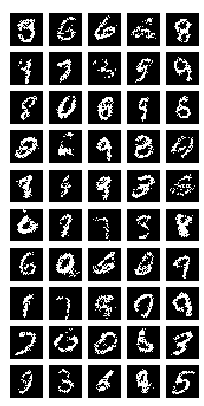
\includegraphics[height=5em]{figs/vae-sample-cropped}
										
\includegraphics[height=5em]{figs/mnist-1}
								};
								\node[right=0.3 of X2, align=center] { %label={left:$\ni$}
										
\includegraphics[height=5em]{figs/mnist-2}
								};
								\fill[opacity=0.2, structurecolor] (X.north east) -- (Z.north west) -- (Z.south west) -- (X.south east) -- cycle;
								\fill[opacity=0.2, structurecolor] (Z.north east) -- (X2.north west) -- (X2.south west) -- (Z.south east) -- cycle;
								\draw[arr] (X) to
								 	node[below,inner sep=2pt]{\small encoder}
									node[above,inner sep=2pt]{$e(Z\mid X)$} (Z);
								\draw[arr] (Z) to
									node[below]{\small decoder}
									node[above]{$d(X \mid Z)$} (X2);
							\end{tikzpicture}
							\end{center}
	            \item Objective:
	            \begin{itemize}
	                \item For each $x$, want to minimize
										% ``reconstruction error'' for each $x$ \\[-1em]
	                    % \[ \mathrm{Rec}(x) = \Ex_{z \sim e \mid x} \underbrace{~\mathrm I_{d\mid z}(x)~}_{\substack{\text{Additional bits to}\\\text{specify $x$ from $d|z$}}}
	                	%    = \sum_z e(z \mid x) \log \frac1{d(x \mid z)} \]
	                    % \[ \mathrm{Rec}(x) = - \Ex_{z \sim e \mid x} \log {d(x \mid z)} \]
	                  $\displaystyle
											\mathrm{Rec}(x) :=
												\overset{\smash{\mathclap{\text{\tiny\color{gray}``reconstruction error'' }}}}
												{ -\!\! \Ex_{z \sim e \mid x}\! \log {d(x \mid z)}} $
	                \vspace{-0.2em}
	                \item Also have a distribution $p(Z)$ that we want encodings to match.
	                    % (Uncorrelated features are more useful.)
	                \item Combine to get VaE objective:\\[0.4em] $\mathrm{ELBO}_{p,e,d}(x) :=$
										\\[-2.1em]
								  \onslide<+->{
	                	\[~~
										 -{\color{gray!80}\underbrace{\usebeamercolor[fg]{normal text} \kldiv[\big]{e(Z|x)}{p(Z)}}_{\smash{\text{\tiny divergence from prior}}}}
									   \onslide<+->{ - \mathrm{Rec}(x)}
										 \onslide<+->{= \!\!\Ex_{z \sim e|x}\! \left[\log \frac{p(z) d(x\mid z)}{e(z\mid x)}\right]}
	                    \onslide<+->{\alert<.>{\le
												\overset{{\color{gray!80}\smash{\text{\tiny ``evidence''}}}}
												{\log \Pr\nolimits_{pd}(x)}%
											}}
									 \]}
	            \end{itemize}
	        \end{itemize}
	    % \column{0.16\linewidth}
	    %     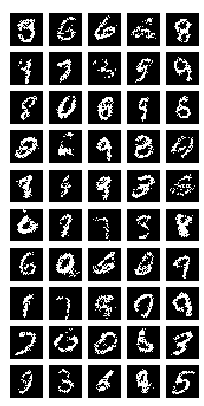
\includegraphics[width=\linewidth]{figs/vae-sample-cropped}
	    %     % 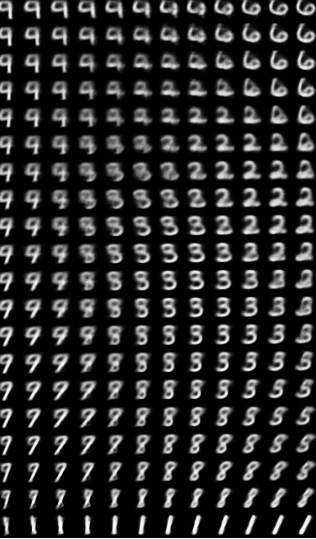
\includegraphics[width=\linewidth]{figs/vae2-cropped}
	    % \end{columns}
			\vspace{-0.7em}

	    \pause[\thebeamerpauses]
	    \alert<.(1)-.(3)>{
					Urge to use graphical models (even if can't quite capture \emph{entire} VaE)}
	    \setlength{\fboxsep}{0pt}
	    \pause\Put(-330,180){\color{structurecolor}\fbox{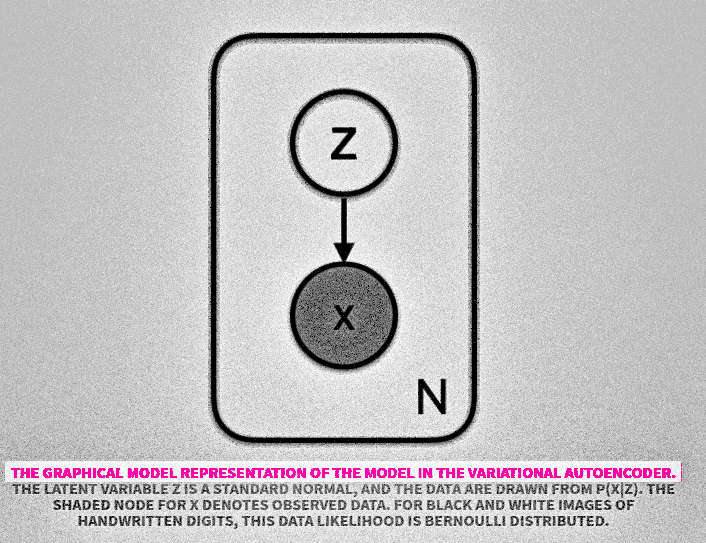
\includegraphics[height=5cm]{figs/vae-diagram-2-colored}}}
	    \pause\Put(-180,185){\color{structurecolor}\fbox{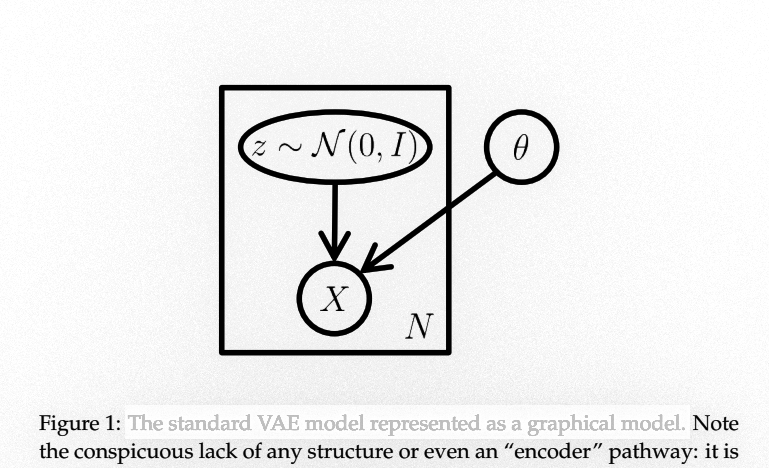
\includegraphics[height=4cm]{figs/vae-diagram-3-uncolored}}}
	    %
			\onslide<+(3)->{
				\Put(-230,195){\color{structurecolor}\fbox{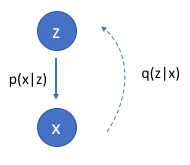
\includegraphics[height=3cm]{figs/vae-diagram-1-cropped}}}%
			}%
	    % \pause
	    % \Put(10,0){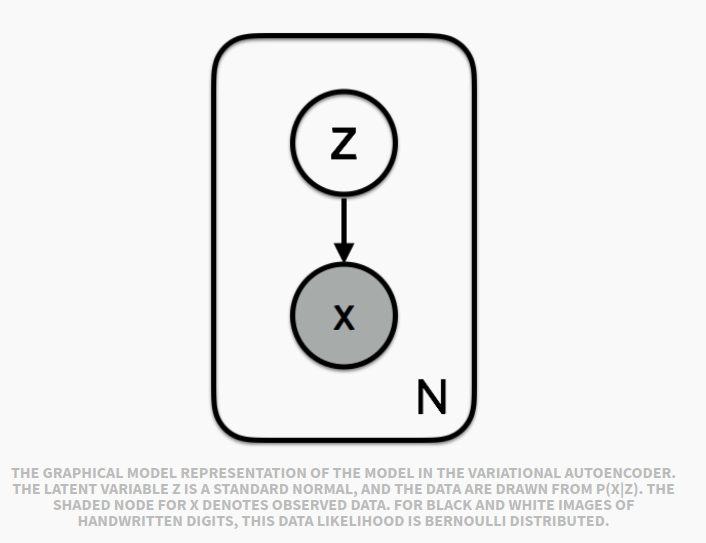
\includegraphics[height=3cm]{figs/vae-diagram-2}}
	    \begin{itemize}[<+-|alert@+>]
	        \item $e(Z\mid X)$ has same target as $p(Z)$, so can't put in BN;
	        \item The heart of the VaE is not its structure, but its objective.
	    \end{itemize}
			% \pause
		\end{frame}

	\begin{frame} \frametitle{Variational Auto-Encoders, Take 2}
			\begin{columns}[c]
			\column{0.38\textwidth}
	    \begin{itemize}[<+-|alert@+>]
	        \item Structure:
	        \begin{description}
	            % \item generate samples of $X$ from a (smaller) latent space $Z$:
	            \item[$e(Z\mid X)$]: encoder
							 	% encodes $X$ in a latent space $Z$;
	            \item[$d(X\mid Z)$]: decoder
								% generate samples of $X$ from $Z$.
	            \item[$p(Z)$]: prior
								% a prior over from $Z$.
	        \end{description}
	        \item observe a sample $x$
					% \begin{itemize}
					% 	\item and trust encoding
					% \end{itemize}
	    \end{itemize}

			\column{0.60\textwidth}
			\onslide<7->{
	    \alert<7>{Objective function is free:}}
	    \[
					\usebeamercolor{alerted text}
					\color<7>{fg}
	        \alt<7->{\aar**}{\hspace{5ex}}{
						\usebeamercolor{normal text}
						\color<7>{fg}\hspace{-1.5em}
						\begin{tikzpicture}[center base]
	            \node[dpad0] (Z) {$Z$};
	            \node[dpad0,right=.9 of Z] (X) {$X$};
	            \onslide<2->{
	                \draw[arr2, ->, onslide=<2>{alertcolor}] (X)
									 		to[bend left=60, looseness=1]
									 		% to[in=-70,out=-110, looseness=1]
											%% v1: exclamation point
	                    % node[below]{$e\onslide<5->{\alert<5>{!}}$} (Z); }
											%% v2: gray ^(\infty)
	                    % node[below, inner sep=1pt]{$e\color{gray}\onslide<6->{\alert<6>{^{\mathrlap{(\only<6>{\beta{:}}\infty)}}}}$} (Z); }
											%% v3: gray infinity, separate node.
	                    node[below]{$e$}
											node[above, inner sep=2pt]{$\lgss\onslide<6->{\alert<6>{(\only<6>{\beta{:}}\infty)}}$}
											%% v4: gray infinity above, except on first show, then with e
	                    % node[below, inner sep=2pt]{$e\only<6>{\mathrlap{\lgss\alert{(\beta{:}\infty)}}}$}
											% node[above, inner sep=2pt]{$\lgss\onslide<7->{(\infty)}$}
										(Z); }
	            \onslide<3->{
	                \draw[arr2, ->, onslide=<3>{alertcolor}] (Z)
											% to[bend left=50]
											to[bend left=60, looseness=1]
	                    node[above]{$d$} (X); }
	            \onslide<5->{
	                \draw[arr2, <<-, onslide=<5>{alertcolor}] (X) --
	                    node[above,pos=0.8]{$x$}
	                    ++(0.9, 0);}
	            \onslide<4->{
	                \draw[arr2, <-, onslide=<4>{alertcolor}] (Z) --
	                    node[above,pos=0.6]{$p$}
	                    node[below=1pt,pos=0.6]{\only<9>{$\color{alertcolor}\scriptscriptstyle(\beta?)$}}
	                    ++(-0.9, 0);}
	        \end{tikzpicture}\!\!\!}
					\onslide<7->{
						 = \mathrm{ELBO}_{p,e,d}(x) }
					% \alert<6>{\;= \mathrm{ELBO}_{p,e,d}(x)}
	    \]
			\end{columns}

			\bigskip
			\onslide<8->{
			\usebeamercolor{alerted text} \color<8>{fg}
			\[=~ \aar**{
			\usebeamercolor{normal text} \color<8>{fg}
			\begin{tikzpicture}[center base]%transform canvas={scale=1}
				\node[dpadded, outer sep=0pt, minimum height=5em] (X) at (0,0) {$X$};
				\node[dpadded, outer sep=0pt, minimum height=2.5em] (Z) at (3,0) {$Z$};
				\node[dpadded, outer sep=0pt, minimum height=5.5em] (X2) at (6,0) {$\hat X$};
				\fill[opacity=0.05, structurecolor] (X.north east) -- (Z.north west) -- (Z.south west) -- (X.south east) -- cycle;
				\fill[opacity=0.05, structurecolor] (Z.north east) -- (X2.north west) -- (X2.south west) -- (Z.south east) -- cycle;
				\draw[arr] (X) to
				 	% node[below,inner sep=2pt]{\small encoder}
				 	node[below,inner sep=2pt]{{$\scriptscriptstyle\color{gray}(\infty)$}}
					node[above,inner sep=2pt]{$e(Z\mid X)$} (Z);
				\draw[arr] (Z) to
					% node[below]{\small decoder}
					node[above]{$d(X \mid Z)$} (X2);
				%
				\draw[arr2, <<-] (X.west) -- node[above,pos=0.6]{$x$} ++(-0.6, 0);
				\draw[arr2, <<-] (X2.east) -- node[above,pos=0.6]{$x$} ++(0.6, 0);
				\draw[arr2, <-] (Z.north) -- node[left,pos=0.6]{$p$} ++(0, 0.6);
				% \draw[arr, double equals sign distance] (X) to[bend right] (X2);
			\end{tikzpicture}}
			\]}
		\end{frame}


	\begin{frame} \frametitle{Visual Proof: The Variational Bound}
			%% Visual proof: VaE Variational Bound
	    \begin{align*}
	    	\onslide<3->{- \log \Pr\nolimits_{p,d}(X\!=\!x) ~=\hspace{0.8in}&\\[-1.3em]
	    	\aar*{\begin{tikzpicture}[center base]
	    	   \node[dpad0] (Z) {$Z$};
	    	   \node[dpad0,right=.6 of Z] (X) {$X$};
	    	   \draw[arr2, ->] (Z) to[bend left=20]
	    		   node[above]{$\scriptstyle d$} (X);
	    	   \draw[arr2, <<-] (X) --
	    		   node[above,pos=0.8]{$\scriptstyle x$}
	    		   ++(0.9, 0);
	    	   \draw[arr2, <-] (Z) --
	    		   node[above,pos=0.6]{$\scriptstyle p$}
	    		   ++(-0.9, 0);%
	    	\end{tikzpicture}}}
	     	&{\onslide<4->{\color{Emerald!50!black}~\le~}}
				\onslide<2->{
		     	\aar*{\begin{tikzpicture}[center base]
		    		\node[dpad0] (Z) {$Z$};
		    		\node[dpad0,right=.5 of Z] (X) {$X$};
		    		\draw[arr2, ->] (X) to[bend left=50]
		    			node[below]{$\scriptstyle e!$} (Z);
		    		\draw[arr2, ->] (Z) to[bend left=50]
		    			node[above]{$\scriptstyle d$} (X);
		    		\draw[arr2, <<-] (X) --
		    			node[above,pos=0.8]{$\scriptstyle x$}
		    			++(0.9, 0);
		    		\draw[arr2, <-] (Z) --
		    			node[above,pos=0.6]{$\scriptstyle p$}
		    			++(-0.9, 0);%
		    	\end{tikzpicture}}
	        \\[-0.7em]&\hspace{1.2in}=~ -\mathrm{ELBO}_{p,e,d}(x).}
	    \end{align*}
			\gdef\customnav{\hyperlink{dpiframe}{\beamergotobutton{Another Visual Proof: Data Processing Inequality}}}
		\end{frame}
	\gdef\customnav{}

\begin{frame} % Summary
	\frametitle{Recap}
	%	\TODO[update with second half]
	PDGs\textellipsis
	\begin{itemize}[<+-|alert@+>]
		\item capture inconsistency, including conflicting information
		from multiple sources with varying reliability.
		\item
		are especially modular.
		%to combine info from two sources, simply take a PDG union.
		%This incorporates new data (edge cpds) and concepts (nodes) without affecting previous information.
		\item cleanly separate quantitative from qualitative information,
		and can express variable confidence in each ($\beta$ and $\alpha$).
		% This is captured by terms $\Inc$ and $\IDef{}$ in our scoring function.
		\item naturally capture BNs and factor graphs, with the best-scoring distribution.
		% In the latter case, a simple parameter shift in the corresponding PDG eliminates
		% arguably problematic behavior of a factor graph.
		\item simultaneously capture many standard loss functions and divergences with the value of the scoring function.
		\item give us a clean visual language for reasoning about the relationships between objectives.
	\end{itemize}

	\pause[\thebeamerpauses]
	\medskip
	\textit{But there is much more to be done!}
\end{frame}




\section{Other Aspects of PDGs}

\subsection{Category Theory}

\begin{frame}[label=commdiagframe]
	\begin{center}
	\only<2>{Commutative diagram~~}
	\only<3>{PDG ~~ $\dg M:=$~~}
	\begin{tikzpicture}[center base]
		\begin{scope}[every node/.style={onslide=<3>{dpadded}}]
			\node (A) at (0,2) {$A$};
			\node (B) at (2,2) {$B$};
			\node (C) at (0,0) {$C$};
			\node (D) at (2,0) {$D$};
		\end{scope}
		\draw[arr2] (A) to node[above]{$f$} (B);
		\draw[arr2] (A) to node[left]{$g$}(C);
		\draw[arr2] (B) to node[right]{$k$} (D);
		\draw[arr2] (C) to node[below]{$h$} (D);
	\end{tikzpicture}
	\only<2>{~~~says ~ $\forall a.~k\!fa = hga$.}
	\only<3>{\hspace{2cm}~}
	\end{center}
	% \[ \exp \left( -\frac1\gamma \aar{\dg M}_\gamma \right) = \parbox{2in}{\raggedright number of bits required \\} \]
	\pause
	
	\onslide<3->{	
%		\begin{itemize}
%			\item 
%		\end{itemize}

		PDG inconsistency measures how close the diagram is to commuting
		\[ \exp \left( -\frac1\gamma \aar{\dg M}_\gamma \right) = \#\Big\{ a : k\!fa = hga \Big\} \]
	}
		% \qquad = - \log \#\{a : kfa = hga \} \]
	% \pause
	% \[ \SD{\dg M}(\mu) = \I[ kfa = hga ] = \qquad - \log \#\{a : kfa = hga \} \]

	\gdef\customnav{\hyperlink{catdef}{\beamergotobutton{More Category Theory}}}
\end{frame}
	\gdef\customnav{}

\subsection{Databases}

\begin{frame} % Databases
	\begin{center}
		% \subcaptionbox{ The three tables of $\D$\label{subfig:tables} }{
		\begin{tikzpicture}[baseline=0, tablename/.style={inner sep=1pt,circle,text=black,font={}},paperfig, scale=0.8]
		%fill=gray!20
		\node at (1,1.5){\textbf{Database}};

		\node[tablename] (R1) at (-1.3,1.2) {\large$\mathbf R_1$};
		\node[below right=-0.2em and -1.2em of R1] (table1) {
			\begin{tabular}{ccc@{}}
			$A$ & $B$ & $C$\\\hline
			$a_1$ & $b_1$ & $c_1$ \\ $a_2$ & $b_2$ & $c_2$
			\end{tabular}
		};
		\draw[] ($(R1.south)+(.3,.1)$) -- ++(-0.3,-0.15) -- ++(0,-1);
		\draw[] ($(R1.south)+(.28,.12)$) -- ++(-0.3,-0.15) -- ++(0,-1);
		\fill[white] ($(R1.south)+(.29,.12)+(-0.3,-0.15)$) rectangle ++(-0.1,-1);


		\node[tablename] (R3) at (-0.5,-0.8) {\large$\mathbf R_3$};
		\node[below right=-0.6em and -0.6em of R3] (table1) {
			\begin{tabular}{cc@{}}
			$C$ & $D$\\\hline
			$c_2$ & $d_1$ \\ $c_1$ & $d_3$
			\end{tabular}
		};
		\draw[] ($(R3.south east)+(.2,.1)$) -- ++(-0.2,-0.2) -- ++(0,-1);
		\draw[] ($(R3.south east)+(.18,.12)$) -- ++(-0.2,-0.2) -- ++(0,-1);
		\fill[white] ($(R3.south east)+(.19,.12)+(-0.2,-0.2)$) rectangle ++(-0.1,-1);

		%        \node[draw,circle,inner sep=0.2pt,fill=gray!50] (R2) at (1.3,1) {\large$R\mspace{-3.5mu}R_2$};
		\node[tablename] (R2) at (1.6,0.7) {\large$\mathbf R_2$};%\mspace{-12.5mu}R
		\node[below right=-0.2em and -1.2em of R2] (table2) {
			\begin{tabular}{cc@{}}
			$B$ & $D$ \\\hline
			$b_2$ & $d_1$ \\ $b_3$ & $d_2$ \\
			$b_4$ & $d_3$
			\end{tabular}
		};
		\draw[] ($(R2.south)+(.3,.1)$) -- ++(-0.3,-0.15) -- ++(0,-1.6);
		\draw[] ($(R2.south)+(.28,.12)$) -- ++(-0.3,-0.15) -- ++(0,-1.6);
		\fill[white] ($(R2.south)+(.29,.12)+(-0.3,-0.15)$) rectangle ++(-0.1,-1.6);
		\end{tikzpicture}
		% }
		 \hfill\vline\hfill
		% \subcaptionbox{ Its schema $\Sch^\D$, as an undirected hypergraph\label{subfig:schema}}{
		\begin{tikzpicture}[paperfig, scale=0.8]
		\node at (0,1.5) {\textbf{Relational Schema}};
		\node[dpadded] (A) at (-2,-0.4){$A$};
		\node[dpadded] (B) at (-0.5, 0.5){$B$};
		\node[dpadded] (C) at (-0.5,-1.3){$C$};
		\node[dpadded] (D) at (1.3,0.3){$D$};

		\coordinate (ABC) at (barycentric cs:A=1,B=1,C=1);
		\node[above left=1pt and -4pt of ABC]{$R_1$};

		\draw[arr, -, shorten >=0, shorten <=1.5pt] (A) -- (ABC) (B) -- (ABC) (C) -- (ABC);
		\draw[arr, -, shorten >=0] (D) -- node[above]{$R_2$} (B);

		\draw[arr, -, shorten >=0] (D) -- node[below right]{$R_3$} (C);
		\end{tikzpicture}
		% }
		 \hfill\vline\hfill
		% \subcaptionbox{ The PDG $\PDGof{\D}$\label{subfig:indexed}}{
		\begin{tikzpicture}[paperfig,scale=0.8]
		\node at (1.5,1.5) {\textbf{Row-PDG}};
		\node[dpadded] (A) at (-0.6,-1.2){$A$};
		\node[dpadded] (C) at (1.4,-1.5){$C$};
		\node[dpadded] (B) at (0.5, 0.5){$B$};
		\node[dpadded] (D) at (3.0,0.6){$D$};

		\node[dpadded,inner sep=2pt] (R1) at (barycentric cs:A=1,B=1.5,C=1){$R_1$};
		\node[dpadded,inner sep=2pt] (R2) at (barycentric cs:B=1,D=1){$R_2$};
		\node[dpadded,inner sep=2pt] (R3) at (barycentric cs:C=1,D=1){$R_3$};
		% \node[above left=1pt and -4pt of ABC]{$R_1$};

		\begin{scope}[->, thick, shorten <=0pt, shorten >=0pt]
		\draw (R1) -- (A);
		\draw (R1) -- (B);
		\draw (R1) -- (C);
		\draw (R2) -- (B);
		\draw (R2) -- (D);
		\draw (R3) -- (D);
		\draw (R3) -- (C);
		\end{scope}
		\end{tikzpicture}
		% }
	\end{center}


	\begin{prop}
		If $\D$ is a database and $\mu$ is a joint distribution over $\PDGof{\D}$, then
		$\mu \in \SD{\PDGof{\D}}$ iff $\mathit{Supp}(\mu) $ is a universal relation for $\D$.
	\end{prop}
	\begin{coro}
		$\PDGof{\D}$ is consistent iff $\D$ is join consistent.
	\end{coro}
\end{frame}
\subsection{Other Projects Work}
\begin{frame}\frametitle{Ongoing and Future Work}
	% \TODO
	\begin{itemize}[<+->]
		\item Belief propagation as local inconsistency reduction
		\item Properties of ``sub-stochastic'' PDGs: semantics for incomplete cpds
		\item Trace Semantics and Composition
		\begin{itemize}
			\item Extend semantics to score other objects, not just joint distributions.
			\item Regarding PDGs as probabilistic automata.
			\item Open Question: Do PDGs capture Dependency Networks? $\ast$
		\end{itemize}
		\item Encoding preferences, and understanding preference changes
		%				\item Multi-agent systems.
	\end{itemize}
\end{frame}



\begin{frame}[label=current]
	\frametitle{A Different Flavor of Agent}
	%% Draw:
	% - many variables, edges
	% - belief in good
	% - multiple agents
	%
	%% Points I want to make (maybe bullets)
	% - Driven by pursuit of a coherent identity, not by maximization of fixed quantity
	% - Can be
	% - Explains (variance in behavior?)

	\begin{center}
		% \begin{tikzpicture}
		% 	\node[dpadded] (W) at (0,0) {$W$};
		% 	\node[dpadded] (O) at (2,0) {$\Omega$};
		% 	\node[dpadded] (A) at (0.8,1) {$A$};
		% 	\node[dpadded] (U) at (3.8,0) {$U$};
		% 	%
		%
		% 	\mergearr[->>] WAO
		% 	\draw[arr2, ->>] (O) -- node[above]{$u$}  (U);
		% \end{tikzpicture}
		\begin{tikzpicture}
			\node[dpadded,outer sep=2pt] (A) at (0.8,1) {$A$};
			\node[dpadded] (U) at (3.8,0) {$U$};
			\onslide<-3>{
					\node[dpadded] (O) at (2,0) {$\Omega$};
					\draw[arr2, ->] (O) -- node[above]{$u$}  (U);
				}
			%
			\onslide<-2>{
		 			\node[dpadded] (W) at (0,0) {$W$};
					\draw[arr2, <-] (W) -- node[above]{$p$} ++(-1.5, 0);
					\mergearr[->] WAO
				}
			\onslide<3->{
					\begin{scope}[every node/.style={dpadded, outer sep=0pt, inner sep=3pt}] %X1, X2, X3
						\node (X1) at (-1.4, -0.3) {$X_1$};
						\node (X2) at (-0.25,-1.2) {$X_2$};
						\node (X3) at (0,0) {$X_3$};
						\end{scope}
					\node[dpadded, % (new W)
							fit={(X1)(X2)(X3)},dashed,
							label={[label distance=-0.8em,%
								fill=white, rounded corners=5,inner sep=0pt]123:$W$},
							fill opacity=0.05,draw opacity=0.2,inner sep=4pt] (newW) {};

					\draw[arr2] (X1) to[bend right] (X2);
					\mergearr {X2}{X3}{X1}
					\draw[arr2, <-] (X1) -- ++(-0.1, -0.8);
					% New merge arrow from worlds + actions -> outcomes
					\onslide<3>{
						% \mergearr A{X3}O
						\coordinate (center1) at (0.8,0.0);
						\coordinate (center2) at (1.0,0.1);

						\draw[arr, -, shorten >=0pt] (X2) to[out=0, in=-110] (center1);
						\draw[arr, -, shorten >=0pt] (X3) to[out=0, in=-170] (center1);
						\draw[arr, -, shorten >=0pt,shorten <=0pt]
							(center1) to[out=20, in=180] (center2);
						\draw[arr, -, shorten >=0pt] (A) to[out=-90, in=150] (center2);
						\draw[arr, ->, shorten <=0pt] (center2) -- (O);
					}
				}
			\onslide<4-> {
				\begin{scope}[every node/.style={dpadded, outer sep=0pt, inner sep=3pt}]
					\node (X4) at (1.7,-0.9) {$X_4$};
					\node (X5) at (2,0) {$X_5$};
					% \node (X6) at (2.2, -0.7) {$X_6$};
				\end{scope}
				\node[dpadded, % (new O)
					fit={(X4)(X5)},dashed,
					label={[label distance=-0.7em,%
						fill=white, rounded corners=3,inner sep=0pt]-65:$\Omega$},
						fill opacity=0.05,draw opacity=0.2,inner sep=4pt] (newO) {};
				\mergearr {X2}{X3}{X4}
				\mergearr {A}{X3}{X5}
				%
				\onslide<4>{
					\mergearr{X4}{X5}{U} }
			}
			\onslide<5->{
				\draw[arr2] (X4) to[bend right=15] (U);
				\draw[arr2] (X5) -- (U);
			}
			\onslide<6->{
				\draw[arr2] (A) to[bend right] (X1);
			}
			\onslide<2>{
				\draw[arr2,line width=0.3pt,gray!70,<-]
					(U) -- node[above]{\tiny faith} ++ (1.5,0);
			}
		\end{tikzpicture}
	\end{center}


	\begin{itemize}
		% \item decompose states and beliefs (like PGMs)
		\item<7-> 
%		Driven by pursuit of cohesive identity;\\ 
		Driven by pursuit of coherence;\\ 
		not (necessarily) maximization.
	\end{itemize}


	\vfill
	\onslide<8->{
		PDG Python library available at~~ \url{https://orichardson.github.io/pdg/}
	}

\end{frame}


\appendix


\section{Hyper-graphs}
	\colorlet{hypergraphcolor}{benchcolor1}
	\colorlet{simplegraphcolor}{structurecolor}
	% \setbeamercolor{background canvas}{bg=black}
	%  \setbeamercolor{normal text}{fg=white}
	%  \usebeamercolor[fg]{normal text}

	\begin{frame}[label=hypergraphextra] %%%%%         HYPER-GRAPHS AND GRAPHS      %%%%%%
		\frametitle{{\color{hypergraphcolor}Hyper-graphs?} Or merely {\color{simplegraphcolor!85}graphs}?}

		\hfill
		\begin{tikzpicture||precompiled}[center base,draw=hypergraphcolor]{grok-pre}
			\fill[fill opacity=0.07,hypergraphcolor, draw, draw opacity=0.2]
				(-0.6,0.6) rectangle (2.1, -2.1);

			\node[dpadded] (C) at (0,0) {$\mathit C$};
			\node[dpadded] (T) at (1.5,0){$\mathit T$};
			\node[dpadded] (SL) at (.75,-1.5){$\it SL$};

			\draw[arr] (T) to[bend right]  (C);
			\alert<2>{ \mergearr{C}{T}{SL} }
			% \drawbb
			\end{tikzpicture||precompiled}
		\onslide<2->{
			\hfill
			\begin{tikzpicture||precompiled}[center base]{widget}%[center base]
			\fill[fill opacity=0.07,simplegraphcolor, draw, draw opacity=0.2]
				(-2.1,-1.85) rectangle (2.1, 1.6);

				\node[dpadded] (SL) at (0,-1.3) {$\mathit{SL}$};

				\node[dpadded] (C) at (-1.5,1) {$\mathit C$};
				\node[dpadded] (T) at (1.5,1) {$\mathit T$};

				\alert<2>{
					\node[dpadded,light pad] (CT) at (0, 0){$\scriptstyle C \times T$};
					\draw[arr1, ->>] (CT) -- (C);
					\draw[arr1, ->>] (CT) -- (T);
					\draw[arr1] (CT) -- (SL);
					}
				\draw[arr] (T) to [bend right=15] (C);
				% \drawbb
				\end{tikzpicture||precompiled}
			}
			\hfill~
		\onslide<3->{
			\vspace{1em}
			\begin{itemize}
				\item<3-|alert@+> This widget expands state space, but graphs are simpler.
				\item<4-> \alert<4>{There is a natural correspondence}
				\[ \text{\color{hypergraphcolor} joint distributions}\quad\leftrightarrows\quad\parbox{15em}{\color{simplegraphcolor}\centering expanded joint distributions\\ satisfying coherence constraints} \]
			\end{itemize}
			}
		\onslide<5->
			{\small\color{gray} (working directly with hypergraphs is also possible)}

		% \vskip0pt plus 1filll
		\gdef\customnav{\hyperlink{definition}{\beamerreturnbutton{main definition}}}
		\end{frame} %----------
		\gdef\customnav{}


\section{The Information Deficiency}
	\begin{frame}[label=idefextra]\frametitle{Illustrations of $\IDef{}$}
		\def\vsize{0.4}
		\begin{center}
		% \vskip0pt plus 1filll
		% \tikzset{dpad0/.append style={fill opacity=0.1}}
		\begin{tikzpicture}[center base,scale=1.5] %\label{subfig:justXY}
			% \node[dpad0] (1) at (0,2){$\pdgunit$};
			\node[dpad0] (X) at (-0.45,.85){$X$};
			\node[dpad0] (Y) at (0.45,.85){$Y$};
			\path[fill=green!50!black] (-0.2,0) circle (\vsize) ++(-110:.26) node[label=below:\tiny$X$]{};
			\path[fill=green!50!black] (0.2,0) circle (\vsize) ++(-70:.26) node[label=below:\tiny$Y$]{};
			\begin{scope}
				\clip (-0.2,0) circle (\vsize);
				\clip (0.2,0) circle (\vsize);
				\fill[green!50!black] (-1,-1) rectangle (3,3);
				% \draw[ultra thick,white] (-0.2,0) circle (\vsize);
				% \draw[ultra thick,white] (0.2,0) circle (\vsize);
			\end{scope}
			\draw (-0.2,0) circle (\vsize);
			\draw (0.2,0) circle (\vsize);
			\useasboundingbox (current bounding box);
			\node at (-0.8, 0.4){};
			\end{tikzpicture}$\qquad$\pause
		%% EXAMPLE: X -> Y
		\begin{tikzpicture}[center base,scale=1.5]%\label{subfig:XtoY}
			% \node[dpad0] (1) at (0,2){$\pdgunit$};
			\node[dpad0] (X) at (-0.45,0.85){$X$};
			\node[dpad0] (Y) at (0.45,0.85){$Y$};
			\draw[arr] (X) to[] (Y);
			% \draw[arr] (1) to[] (Y);
			\path[fill=green!50!black] (-0.2,0) circle (\vsize) ++(-110:.26) node[label=below:\tiny$X$]{};
			\path[fill=white!70!black] (0.2,0) circle (\vsize) ++(-70:.26) node[label=below:\tiny$Y$]{};
			\begin{scope}
				\clip (-0.2,0) circle (\vsize);
				\clip (0.2,0) circle (\vsize);
				\fill[green!50!black] (-1,-1) rectangle (3,3);
				% \draw[ultra thick,white] (-0.2,0) circle (\vsize);
				% \draw[ultra thick,white] (0.2,0) circle (\vsize);
			\end{scope}
			\draw (-0.2,0) circle (\vsize);
			\draw (0.2,0) circle (\vsize);
			\useasboundingbox (current bounding box);
			\node at (-0.8, 0.4){};
			\end{tikzpicture}$\qquad$\pause
		%% EXAMPLE: X ->> Y
		\begin{tikzpicture}[center base,scale=1.5]%\label{subfig:XtoY}
			% \node[dpad0] (1) at (0,2){$\pdgunit$};
			\node[dpad0] (X) at (-0.45,0.85){$X$};
			\node[dpad0] (Y) at (0.45,0.85){$Y$};
			\draw[arr,->>] (X) to[] (Y);
			% \draw[arr] (1) to[] (Y);
			\path[fill=green!50!black] (-0.2,0) circle (\vsize) ++(-110:.26) node[label=below:\tiny$X$]{};
			\path[fill=red!50!black] (0.2,0) circle (\vsize) ++(-70:.26) node[label=below:\tiny$Y$]{};
			\begin{scope}
				\clip (-0.2,0) circle (\vsize);
				\clip (0.2,0) circle (\vsize);
				\fill[green!50!black] (-1,-1) rectangle (3,3);
				% \draw[ultra thick,white] (-0.2,0) circle (\vsize);
				% \draw[ultra thick,white] (0.2,0) circle (\vsize);
			\end{scope}
			\draw (-0.2,0) circle (\vsize);
			\draw (0.2,0) circle (\vsize);
			\useasboundingbox (current bounding box);
			\node at (-0.8, 0.4){};
			\end{tikzpicture}$\qquad$\pause
		%% EXAMPLE: X <-> Y
		\begin{tikzpicture}[center base,scale=1.5] %\label{subfig:XY-cycle}
			% \node[dpad0] (1) at (0,2){$\pdgunit$};
			\node[dpad0] (X) at (-0.45,0.85){$X$};
			\node[dpad0] (Y) at (0.45,0.85){$Y$};
			\draw[arr] (X) to[bend left] (Y);
			\draw[arr] (Y) to[bend left] (X);
			\draw[fill=white!70!black] (-0.2,0) circle (\vsize) ++(-110:.26) node[label=below:\tiny$X$]{};
			\draw[fill=white!70!black] (0.2,0) circle (\vsize) ++(-70:.26) node[label=below:\tiny$Y$]{};
			\begin{scope}
				\clip (-0.2,0) circle (\vsize);
				\clip (0.2,0) circle (\vsize);
				\fill[green!50!black] (-1,-1) rectangle (3,3);
				% \draw[ultra thick,white] (-0.2,0) circle (\vsize);
				% \draw[ultra thick,white] (0.2,0) circle (\vsize);
			\end{scope}
			\draw (-0.2,0) circle (\vsize);
			\draw (0.2,0) circle (\vsize);
			\useasboundingbox (current bounding box.south west) rectangle (current bounding box.north east);
			\node at (-0.85, 0.4){};
			\end{tikzpicture}
		\end{center}

			% \vskip0pt plus 1filll \hfill
			\gdef\customnav{%
				\hyperlink{returntosemantics}{\beamerreturnbutton{back to semantics}}}
		\end{frame}

	\begin{frame} % More IDef Illustrations
		\def\vsize{0.4}
		\def\bnslide{2}
		\def\spacerlength{0.5em}
		\begin{tikzpicture}[center base]\label{subfig:justX-0}
			\node[dpad0] (X) at (0,1){$X$};
			\draw[fill=green!50!black]  (0,0) circle (\vsize)  ++(-90:.22) node[label=below:\tiny$X$]{};
			\useasboundingbox (current bounding box);
			\node at (-0.5, 0.6){};
			\end{tikzpicture}
		\begin{tabular}{c}
				\begin{tikzpicture}[onslide=<\bnslide>{is bn}]\label{subfig:justX-1}
					\node[dpad0] (1) at (-0.4,.85){$\!\pdgunit\!$};
					\node[dpad0] (X) at (0.4,.85){$X$};
					\draw[arr1] (1)  -- (X);
					\draw[fill=white!70!black]  (0,0) circle (\vsize) ++(-90:.22) node[label=below:\tiny$X$]{};
					\node at (-0.6,0.35){};
					\useasboundingbox (current bounding box);
					\node at (-0.7, 0.35){};
					\end{tikzpicture} \\[0.5em]
				\begin{tikzpicture}\label{subfig:justX-2}
					\node[dpad0] (1) at  (-0.45,.85){$\!\pdgunit\!$};
					\node[dpad0] (X) at  (0.45,.85){$X$};
					\draw[arr1] (1) to[bend left=20] (X);
					\draw[arr1] (1) to[bend right=20] (X);
					\draw[fill=red!50!black] (0,0) circle (\vsize) ++(-90:.22) node[label=below:\tiny$X$]{};
					\useasboundingbox (current bounding box);
					\node at (-0.7, 0.35){};
					\end{tikzpicture}
			\end{tabular}%}
			\hspace{\spacerlength}\vrule\hspace{\spacerlength}
		% \adjustbox{valign=b}{
		\begin{tabular}{c}
				%% EXAMPLE: X  Y
				\begin{tikzpicture}[] \label{subfig:justXY}
					% \node[dpad0] (1) at (0,2){$\pdgunit$};
					\node[dpad0] (X) at (-0.45,.85){$X$};
					\node[dpad0] (Y) at (0.45,.85){$Y$};
					\path[fill=green!50!black] (-0.2,0) circle (\vsize) ++(-110:.23) node[label=below:\tiny$X$]{};
					\path[fill=green!50!black] (0.2,0) circle (\vsize) ++(-70:.23) node[label=below:\tiny$Y$]{};
					\begin{scope}
						\clip (-0.2,0) circle (\vsize);
						\clip (0.2,0) circle (\vsize);
						\fill[green!50!black] (-1,-1) rectangle (3,3);
						% \draw[ultra thick,white] (-0.2,0) circle (\vsize);
						% \draw[ultra thick,white] (0.2,0) circle (\vsize);
					\end{scope}
					\draw (-0.2,0) circle (\vsize);
					\draw (0.2,0) circle (\vsize);
					\useasboundingbox (current bounding box);
					\node at (-0.8, 0.4){};
					\end{tikzpicture}\\[0.5em]
				%% EXAMPLE: X -> Y
				\begin{tikzpicture}[] \label{subfig:XtoY}
					% \node[dpad0] (1) at (0,2){$\pdgunit$};
					\node[dpad0] (X) at (-0.45,0.85){$X$};
					\node[dpad0] (Y) at (0.45,0.85){$Y$};
					\draw[arr1] (X) to[] (Y);
					% \draw[arr] (1) to[] (Y);
					\path[fill=green!50!black] (-0.2,0) circle (\vsize) ++(-110:.23) node[label=below:\tiny$X$]{};
					\path[fill=white!70!black] (0.2,0) circle (\vsize) ++(-70:.23) node[label=below:\tiny$Y$]{};
					\begin{scope}
						\clip (-0.2,0) circle (\vsize);
						\clip (0.2,0) circle (\vsize);
						\fill[green!50!black] (-1,-1) rectangle (3,3);
						% \draw[ultra thick,white] (-0.2,0) circle (\vsize);
						% \draw[ultra thick,white] (0.2,0) circle (\vsize);
					\end{scope}
					\draw (-0.2,0) circle (\vsize);
					\draw (0.2,0) circle (\vsize);
					\useasboundingbox (current bounding box);
					\node at (-0.8, 0.4){};
					\end{tikzpicture}
			\end{tabular}%}
			% \hspace{\spacerlength}
		\begin{tabular}{c}
				%% EXAMPLE: X <-> Y
				\begin{tikzpicture}[center base]\label{subfig:XY-cycle}
					% \node[dpad0] (1) at (0,2){$\pdgunit$};
					\node[dpad0] (X) at (-0.45,0.85){$X$};
					\node[dpad0] (Y) at (0.45,0.85){$Y$};
					\draw[arr1] (X) to[bend left] (Y);
					\draw[arr1] (Y) to[bend left] (X);
					\draw[fill=white!70!black] (-0.2,0) circle (\vsize) ++(-110:.25) node[label=below:\tiny$X$]{};
					\draw[fill=white!70!black] (0.2,0) circle (\vsize) ++(-70:.25) node[label=below:\tiny$Y$]{};
					\begin{scope}
						\clip (-0.2,0) circle (\vsize);
						\clip (0.2,0) circle (\vsize);
						\fill[green!50!black] (-1,-1) rectangle (3,3);
						% \draw[ultra thick,white] (-0.2,0) circle (\vsize);
						% \draw[ultra thick,white] (0.2,0) circle (\vsize);
					\end{scope}
					\draw (-0.2,0) circle (\vsize);
					\draw (0.2,0) circle (\vsize);
					\useasboundingbox (current bounding box.south west) rectangle (current bounding box.north east);
					\node at (-0.85, 0.4){};
					\end{tikzpicture}\\[2.5em]
					% \hspace{\spacerlength}
				%% EXAMPLE: 1 -> Y;1->X
				\begin{tikzpicture}[center base, onslide=<\bnslide>{is bn}] \label{subfig:XYindep}
					\node[dpad0] (1) at (0,0.75){$\!\pdgunit\!$};
					\node[dpad0] (X) at (-0.7,0.95){$X$};
					\node[dpad0] (Y) at (0.7,0.95){$Y$};
					\draw[arr0] (1) to[] (X);
					\draw[arr0] (1) to[] (Y);
					\draw[fill=white!70!black] (-0.2,0) circle (\vsize) ++(-110:.23) node[label=below:\tiny$X$]{};
					\draw[fill=white!70!black] (0.2,0) circle (\vsize) ++(-70:.23) node[label=below:\tiny$Y$]{};
					\begin{scope}
						\clip (-0.2,0) circle (\vsize);
						\clip (0.2,0) circle (\vsize);
						\fill[red!50!black] (-1,-1) rectangle (3,3);
						% \draw[ultra thick,white] (-0.2,0) circle (\vsize);
					% \draw[ultra thick,white] (0.2,0) circle (\vsize);
					\end{scope}
					\draw (-0.2,0) circle (\vsize);
					\draw (0.2,0) circle (\vsize);
					\useasboundingbox (current bounding box.south west) rectangle (current bounding box.north east);
					\node at (-0.88, 0.4){};
					\end{tikzpicture}
			\end{tabular}
			\hspace{\spacerlength}
		 %% EXAMPLE: 1 -> X -> Y
		\begin{tikzpicture}[center base, onslide=<\bnslide>{is bn}]\label{subfig:1XY}
			\node[dpad0] (1) at (0.15,2){$\!\pdgunit\!$};
			\node[dpad0] (X) at (-0.45,1.4){$X$};
			\node[dpad0] (Y) at (0.35,1){$Y$};
			\draw[arr0] (1) to[] (X);
			\draw[arr1] (X) to[] (Y);
			\path[fill=white!70!black] (-0.2,0) circle (\vsize) ++(-110:.23) node[label=below:\tiny$X$]{};
			\path[fill=white!70!black] (0.2,0) circle (\vsize) ++(-70:.23) node[label=below:\tiny$Y$]{};
			\begin{scope}
				\clip (-0.2,0) circle (\vsize);
				\clip (0.2,0) circle (\vsize);
				% \fill[red!50!black] (-1,-1) rectangle (3,3);
				% \draw[ultra thick,white] (-0.2,0) circle (\vsize);
				% \draw[ultra thick,white] (0.2,0) circle (\vsize);					\end{scope}
			\end{scope}
			\draw (-0.2,0) circle (\vsize);
			\draw (0.2,0) circle (\vsize);
			\useasboundingbox (current bounding box);
			\node at (-0.7, 0.6){};
			\end{tikzpicture}
			% \hspace{\spacerlength}\hspace{2.5pt}\vrule\hspace{2.5pt}\hspace{\spacerlength}
		\relax	%CENTER CODE.
			\vspace{0.5em}
			\onslide<bnslide>{\tikz[is bn] \node{Achievable by BN}; }

		%% EXAMPLE: 1 -> X -> Y -> Z
		\begin{tikzpicture}[center base, onslide=<\bnslide>{is bn}] \label{subfig:1XYZ}
			% \node[dpad0] (1) at (-0.5,2.3){$\!\pdgunit\!$};
			% \node[dpad0] (X) at (-0.5,1.5){$X$};
			% \node[dpad0] (Y) at (0.35,1.25){$Y$};
			% \node[dpad0] (Z) at (0.25,2.25){$Z$};
			\node[dpad0] (1) at (-1,0.8){$\!\pdgunit\!$};
			\node[dpad0] (X) at (-0.6,1.6){$X$};
			\node[dpad0] (Y) at (0.35,1.6){$Y$};
			\node[dpad0] (Z) at (1.0,0.9){$Z$};
			\draw[arr0] (1) to (X);
			\draw[arr1] (X) to[] (Y);
			\draw[arr1] (Y) to[] (Z);
			\path[fill=white!70!black] (210:0.22) circle (\vsize) ++(-130:.25) node[label=below:\tiny$X$]{};
			\path[fill=white!70!black] (-30:0.22) circle (\vsize) ++(-50:.25) node[label=below:\tiny$Y$]{};
			\path[fill=white!70!black] (90:0.22) circle (\vsize) ++(40:.29) node[label=above:\tiny$Z$]{};
			\begin{scope}
				\clip (90:0.22) circle (\vsize);
				\clip (210:0.22) circle (\vsize);
				\fill[red!50!black] (-1,-1) rectangle (3,3);
				% \draw[ultra thick,white] (210:0.2) circle (\vsize);
				% \draw[ultra thick,white] (90:0.2) circle (\vsize);
				\clip (-30:0.22) circle (\vsize);
				\fill[white!70!black] (-1,-1) rectangle (3,3);
				% \draw[ultra thick,white] (-30:0.2) circle (\vsize);
				% \draw[ultra thick,white] (210:0.2) circle (\vsize);
				% \draw[ultra thick,white] (90:0.2) circle (\vsize);
			\end{scope}
			\begin{scope}
				\draw[] (-30:0.22) circle (\vsize);
				\draw[] (210:0.22) circle (\vsize);
				\draw[] (90:0.22) circle (\vsize);
			\end{scope}
			\useasboundingbox (current bounding box);
			\node at (-0.7, 0.7){};
			\end{tikzpicture}
			\hspace{\spacerlength}
		%% EXAMPLE: X -> Y -> Z -> X
		\begin{tikzpicture}[center base] \label{subfig:XYZ-cycle}
			% \node[dpad0] (1) at (-0.5,2.3){$\pdgunit$};
			\node[dpad0] (X) at (-0.5,1.75){$X$};
			\node[dpad0] (Y) at (0.35,1.25){$Y$};
			\node[dpad0] (Z) at (0.25,2.25){$Z$};
			% \draw[arr0] (1) to (X);
			\draw[arr1] (X) to[bend right=25] (Y);
			\draw[arr1] (Y) to[bend right=25] (Z);
			\draw[arr1] (Z) to[bend right=25] (X);
			%option: -- either X -> Y -> Z -> X, or <-> Y <-> Z <-> X. For the latter, uncomment the 6 lines below and comment out the next 3.
			% \draw[arr1] (Z) to[bend left=5] (Y);
			% \draw[arr1] (Y) to[bend left=5] (X);
			% \draw[arr1] (X) to[bend left=5] (Z);
			% \draw[fill=red!50!black] (210:0.22) circle (\vsize) ++(-130:.27) node[label=below:\tiny$X$]{};
			% \draw[fill=red!50!black] (-30:0.22) circle (\vsize) ++(-50:.27) node[label=below:\tiny$Y$]{};
			% \draw[fill=red!50!black] (90:0.22) circle (\vsize) ++(140:.31) node[label=above:\tiny$Z$]{};

			% grey filling for one covering.
			\draw[fill=white!70!black] (210:0.22) circle (\vsize) ++(-130:.27) node[label=below:\tiny$X$]{};
			\draw[fill=white!70!black] (-30:0.22) circle (\vsize) ++(-50:.27) node[label=below:\tiny$Y$]{};
			\draw[fill=white!70!black] (90:0.22) circle (\vsize) ++(40:.31) node[label=above:\tiny$Z$]{};

			\begin{scope}
				\clip (-30:0.22) circle (\vsize);
				\clip (210:0.22) circle (\vsize);
				% \fill[white!70!black] (-1,-1) rectangle (3,3);
				\clip (90:0.22) circle (\vsize);
				\fill[green!50!black] (-1,-1) rectangle (3,3);
			\end{scope}
			\begin{scope}
				\draw[] (-30:0.22) circle (\vsize);
				\draw[] (210:0.22) circle (\vsize);
				\draw[] (90:0.22) circle (\vsize);
			\end{scope}
			\useasboundingbox (current bounding box);
			\node at (-0.7, 0.7){};
			\end{tikzpicture}
			\hspace{\spacerlength}
		%% EXAMPLE: X -> Y <- Z
		\begin{tikzpicture}[center base] \label{subfig:XZtoY}
			% \node[dpad0] (1) at (-0.5,2.3){$\pdgunit$};
			\node[dpad0] (X) at (-0.45,1.9){$X$};
			\node[dpad0] (Y) at (0.3,1.25){$Y$};
			\node[dpad0] (Z) at (0.4,2.15){$Z$};
			% \draw[arr0] (1) to (X);
			\draw[arr0] (X) to[] (Y);
			\draw[arr1] (Z) to[] (Y);
			\path[fill=green!50!black] (210:0.22) circle (\vsize) ++(-130:.25) node[label=below:\tiny$X$]{};
			\path[fill=red!50!black] (-30:0.22) circle (\vsize) ++(-50:.25) node[label=below:\tiny$Y$]{};
			\path[fill=green!50!black] (90:0.22) circle (\vsize) ++(40:.29) node[label=above:\tiny$Z$]{};
			\begin{scope}
				\clip (-30:0.22) circle (\vsize);
				\clip (90:0.22) circle (\vsize);
				\fill[white!70!black] (-1,-1) rectangle (3,3);
			\end{scope}
			\begin{scope}
				\clip (-30:0.22) circle (\vsize);
				\clip (210:0.22) circle (\vsize);
				\fill[white!70!black] (-1,-1) rectangle (3,3);

				\clip (90:0.22) circle (\vsize);
				\fill[green!50!black] (-1,-1) rectangle (3,3);
				% \draw[ultra thick,white] (210:0.2) circle (\vsize);
				% \draw[ultra thick,white] (90:0.2) circle (\vsize);
				% \draw[ultra thick,white] (-30:0.2) circle (\vsize);
				% \draw[ultra thick,white] (210:0.2) circle (\vsize);
				% \draw[ultra thick,white] (90:0.2) circle (\vsize);
			\end{scope}
			\draw[] (-30:0.22) circle (\vsize);
			\draw[] (210:0.22) circle (\vsize);
			\draw[] (90:0.22) circle (\vsize);
			\useasboundingbox (current bounding box);
			% \node at (-0.7, 0.7){};
			\end{tikzpicture}
			\hspace{\spacerlength}
		%% EXAMPLE: X <-> Y <-> Z
		\begin{tikzpicture}[center base] \label{subfig:XYZ-bichain}
			% \node[dpad0] (1) at (0.1,2.4){$\pdgunit$};
			\node[dpad0] (X) at (-1,1.2){$X$};
			\node[dpad0] (Y) at (0,1.7){$Y$};
			\node[dpad0] (Z) at (1,1.4){$Z$};
			% \draw[arr1] (1) to (X);
			% \draw[arr1] (1) to (Y);
			\draw[arr1] (X) to[bend right=15] (Y);
			\draw[arr1] (Y) to[bend right=15] (X);
			\draw[arr1] (Y) to[bend right=15] (Z);
			\draw[arr1] (Z) to[bend right=15] (Y);
			\path[fill=white!70!black] (210:0.22) circle (\vsize) ++(-130:.25) node[label=below:\tiny$X$]{};
			\path[fill=red!50!black] (-30:0.22) circle (\vsize) ++(-50:.25) node[label=below:\tiny$Y$]{};
			\path[fill=white!70!black] (90:0.22) circle (\vsize) ++(40:.29) node[label=above:\tiny$Z$]{};
			\begin{scope}
				\clip (-30:0.22) circle (\vsize);
				\clip (90:0.22) circle (\vsize);
				\fill[white!70!black] (-1,-1) rectangle (3,3);
			\end{scope}
			\begin{scope}
				\clip (90:0.22) circle (\vsize);
				\clip (210:0.22) circle (\vsize);
				\fill[red!50!black] (-1,-1) rectangle (3,3);
			\end{scope}
			\begin{scope}
				\clip (-30:0.22) circle (\vsize);
				\clip (210:0.22) circle (\vsize);
				\fill[white!70!black] (-1,-1) rectangle (3,3);

				\clip (90:0.22) circle (\vsize);
				\fill[green!50!black] (-1,-1) rectangle (3,3);
				% \draw[ultra thick,white] (210:0.2) circle (\vsize);
				% \draw[ultra thick,white] (90:0.2) circle (\vsize);
				% \draw[ultra thick,white] (-30:0.2) circle (\vsize);
				% \draw[ultra thick,white] (210:0.2) circle (\vsize);
				% \draw[ultra thick,white] (90:0.2) circle (\vsize);
			\end{scope}
			\draw[] (-30:0.22) circle (\vsize);
			\draw[] (210:0.22) circle (\vsize);
			\draw[] (90:0.22) circle (\vsize);
			\useasboundingbox (current bounding box);
			\node at (-0.7, 0.7){};
			\end{tikzpicture}
		\end{frame}
		\gdef\customnav{}

\section{More on Semantics}
	\begin{frame}[label=more-semantics-properties]
		\begin{prop}[{{\itshape\normalfont {uniqueness for small $\gamma$}}}]
			\begin{enumerate}
			\item If  $0 < \gamma \leq \min_L \beta_L^{\dg M}$, then
			$\bbr{\dg M}_\gamma^*$ is a singleton.
			\item $\displaystyle\lim_{\gamma\to0}\bbr{\dg M}_\gamma^*$ exists and is a singleton.
			\end{enumerate}
		\end{prop}
		\pause
		This lets us define~ $\bbr{\dg M}^* := $
		unique element $\displaystyle\left(\lim_{\gamma\to0} \bbr{\dg M}_\gamma^*\right)$.
		\end{frame}
	\begin{frame}[label=semantics-relationships]
		\frametitle{Relationships Between Semantics}
		\begin{prop}%
				% [{\normalsize{\it $\SD{\dg M}$ is the zero set of $\bbr{\dg M}$\;}}]
				[{\small{\it the set of consistent distributions is the zero set of the scoring function}}]
			$\SD{\dg M} \!= \big\{ \mu : \bbr{\dg M}_0(\mu) \!=\! 0 \big\}$.
			\end{prop}

		\begin{prop}[{\normalsize{\it If there there are distributions consistent
			 		with $\dg M$, the best distribution is one of them.\;}}]
					\label{prop:consist}
				$\bbr{\dg M}^* \in \bbr{\dg M}_0^*$, so if $\dg M$ is consistent,
				then $\bbr{\dg M}^* \in \SD{\dg  M}$.
			\end{prop}

		\gdef\customnav{\hyperlink{semantics-properties}{\beamerreturnbutton{back to semantics properties}}}
		\end{frame}
		\gdef\customnav{}


	\begin{frame}[label=another-semantics]\frametitle{Another View of PDG semantics}
		\[ \bbr{\dg M}_\gamma(\mu) = \Ex_{\mu}\log \prod_{\ed LXY} \left(\frac{\mu(Y\mid X)}{\bp(Y\mid X)}\right)^{\beta\ssub L}
		\;
		\left(\frac{\mu(\N)}{\prod\limits_{\ed LXY} \mu(Y\mid X)^{\alpha\ssub L}}\right)^\gamma
		\]
	\end{frame}

	\begin{frame}[label=another-semantics+fg] %%%%%  SCORING FUNCTION BREAKDOWN  %%%%
		% \begin{prop}\label{prop:nice-score}%
			% Let $x^{\mat w}$, $y^{\mat w}$ denote the values of
			% $X$,$Y$ in world $\mat w$. Then:
			\frametitle{Comparing PDG to Factor Graph Semantics}

			{\small
			\begin{equation*}\label{eq:semantics-breakdown}
				% \begin{split}
					\bbr{\dg M}(\mu) =
					% \Ex_{\mat w \sim \mu}\! \Bigg\{
					\Ex\nolimits_\mu	\!\!
					 \sum_{ X \xrightarrow{\!\!L} Y  }
					\bigg[\,
					    {\color{benchcolor1}\overbrace{\color{black}
					      % \beta_L \log \frac{1}{\bp(y^{\mat w} |x^{\mat w})}
					      \beta\ssub L \log \frac{1}{\bp(Y|X)}
						}^{\color{benchcolor1}\smash{\mathclap{\text{log likelihood / cross entropy}}}}}~+
						 % \qquad\qquad\qquad\\[-0.7em]\qquad\qquad
					    {\color{benchcolor2}\underbrace{\color{black}
					({\alpha \ssub L}\gamma - \beta\ssub L )
							% \log \frac{1}{\mu(y^{\mat w} |x^{\mat w})}
							\log \frac{1}{\mu(Y | X)}
						}_{\color{benchcolor2}\smash{\mathclap{\text{local regularization (if $\beta\ssub L >	\alpha\ssub L
						\gamma$)}}}}}~\bigg] - \color{structurecolor!70!blue}
						\overbrace{\color{black}
					% \gamma \log \frac{1}{\mu(\mat w)}
					\gamma \H(\mu) \vphantom{\Big|}
						}^{\color{structurecolor!70!blue}\smash{\mathclap{\text{%
							% ~~~~global regularization
							global regularization~~~~%
							}}}}\color{black}
									% \Bigg\} .				\end{split}
									.
				\end{equation*}}
			\bigskip

			\pause
			And the weighted factor graph's canonical scoring function:
			\[ \VFE_\Psi(\mu) := \Ex_{\mu} \left[ \sum_{J \in \mathcal J} {\theta_J} \log \frac1{\phi_J(X_J)} \right] - \H(\mu) \]
			% \end{prop}
		\end{frame}

	\begin{frame}[label=minimization-semantics-properties] \frametitle{Properties of Inconsistency, for minimization}

			\[ \aar{\dg M}_\gamma := \inf_\mu \bbr{\dg M}_\gamma \]
			% \begin{prop}

			Nice properties for minimization:
			\begin{itemize}
				\item The function $\gamma\mapsto\aar{\dg M}_\gamma$ is continuous for all $\gamma$
				\item The function $p \mapsto \aar{\dg M \sqcup p}_\gamma$ is smooth and strictly convex on its interior.
			\end{itemize}
				% \end{prop}
		\end{frame}

	\begin{frame}[label=semantics-thermo]
		\[ \VFE_\Phi(\mu) := \Ex_{\mu} \Big[ - \sum_{J \in \mathcal J}
			% \only<7->{\alert<7>{\theta_J}}
			\theta_J
			 \log {\phi_J(X_J)} \Big] - \H(\mu) \]
		\gdef\customnav{\hyperlink{factor-graph-intro}{\beamerreturnbutton{Back to Factor Graph Definition}}}
		\end{frame}
		\gdef\customnav{}

\section{More on Graphical Models}
	\subsection{BNs as MaxEnt}\label{sec:bnmaxent}

	\begin{frame} \frametitle{Bayesian Networks: Maximum Entropy?}
			\begin{columns}[c]
				\small
				\column{0.3\textwidth}
					\centering
					Common distributions tend to maximize entropy subject to natural constraints.

				\column{0.7\textwidth}
					\footnotesize
					\renewcommand\arraystretch{1.2}
					\color{gray}
					\begin{tabular}{r|l}
						\texttt{distribution}&\texttt{constraints}\\\hline
						Gaussian $\mathcal N(\mu, \sigma^2)$ & mean $\mu$, variance $\sigma^2$ \\
						Exponential $\mathrm{Exp}(\lambda)$& positive support, mean $\lambda$ \\
						Factor graphs& moment matching. \\
						$\cdots$ & $\cdots$ \\
						\pause
						\color{black}
						Bayesian Networks & \color{black} cpds + \alert<.(1)>{???}
					\end{tabular}
			\end{columns}
			\pause
			\begin{center}
				\small
				\begin{tikzpicture}[scale=0.9]
					\node[dpadded] (c1) at (0,0.6) {$C_1$};
					\node[dpadded] (c2) at (0,-0.6) {$C_2$};
					\node[dpadded] (X) at (2, 0) {$X$};

					\draw[arr, <-] (c1) -- node[above]{50/50} ++(-2.1, 0);
					\draw[arr, <-] (c2) -- node[above]{50/50} ++(-2.1, 0);
					\cmergearr {c1}{c2}{X}{1,0}
					% \node[below=0.2 of center-c1c2X]{
					\node[right=0.2 of X,align=left]{
						$\Pr(X\mid C_1,C_2)=$\\[0.1em]$\quad\begin{cases}
							\mathbbm{1}{[X=x_0]} & \text{if } C_1 = C_2 \\
							\mathrm{Unif}(X) & \text{if } C_1 \ne C_2
						\end{cases}$
					};
				\end{tikzpicture}
			\end{center}
			\pause

			\begin{coro}
				Among the distributions in $\SD{\mathcal B}$,
				$\Pr_{\mathcal B}$ has the maximum entropy, beyond the entropy of the given cpds.
			\end{coro}
			\vspace{-0.9em}
			\[\text{$\IDef{}$ says maximize:}\quad \H(\mu) - \sum_{X \in \N} \H_\mu( X \mid \Pa\, X ) \]

			% \vspace{-1em}\raggedleft
			% \onslide<1->{\hyperlink{returntobns}{\beamerreturnbutton{back to BN theorem}}}
			\gdef\customnav{\hyperlink{returntobns}{\beamerreturnbutton{back to BN theorem}}}
			\end{frame}
			\gdef\customnav{}

	\begin{frame} \frametitle{Full Factor Graph Results}
		\begin{theorem}[PDGs are WFGs]\label{thm:pdg-is-wfg}
			If $\boldsymbol\beta = \gamma\boldsymbol\alpha $, then
			$\bbr{\dg M}^*_\gamma = \Pr_{(\Phi_{\dg M}, \boldsymbol\beta)}$.


			Concretely, for all unweighted PDGs $\dg{N}$ and non-negative vectors $\mat v$
			over the edges of $\dg N$, and all $\gamma > 0$, we have that
			$\bbr{(\dg N, \mat v, \gamma \mat v)}_{\gamma}
			= \gamma\,\VFE_{(\Phi_{\dg N}, \mat v)} $; consequently,
			$\bbr{(\dg N,  \mat v,  \gamma\mat v)}_{\gamma}^*
					= \{\Pr_{(\Phi_{\dg N}, \mat v)} \}$.
		\end{theorem}

		\begin{theorem}[WFGs are PDGs]\label{them:wfg-is-pdg}
			For all weighted factor graphs $\Psi = (\Phi,\theta)$ and all $\gamma > 0$,
			we have that
			$\VFE_\Psi
			= \nicefrac1{\gamma} \bbr{{\dg M}_{\Psi,\gamma}}_{\gamma}
			+ C$
			for some constant $C$, so
			$\Pr_{\Psi}$ is the unique element of
			$\bbr{{\dg M}_{\Psi,\gamma}}_{\gamma}^*$.
			\end{theorem}

		\gdef\customnav{%
			\hyperlink{returnto-pdg-is-wfg}{\beamerreturnbutton{PDG$\to$WFG}}
			\hyperlink{returnto-pdg-is-wfg}{\beamerreturnbutton{WFG$\to$PDG}}
		}%
		\end{frame}
		\gdef\customnav{}


\section{More Losses}
\begin{frame} %% Marginal Surprise as Inconsistency
    \frametitle{Variations: Surprise as Inconsistency}
    % For partial observations
    \begin{prop}[marginal information as inconsistency]<+-|alert@+>
        If $p(X,Z)$ is a joint distribution, the (marginal) information of the (partial) observation $X=x$ is given by\\[-1.0em]
    % Marginal Information:
        \[
    	 	\I_p(x) = \log \frac{1}{p(x)} =
    		 \aar[\Bigg]{
    			\begin{tikzpicture}[center base]
    				\node[dpad0] (Z) {$Z$};
    				\node[dpad0,right=.5 of Z] (X) {$X$};
    				\coordinate (A) at ($ (X)!.5!(Z) + (0,0.7)$);
    				\draw[arr1] (A) -- node[right]{$\scriptstyle p$} ++(0,-0.25) -- (X);
    				\draw[arr1] (A) -- ++(0,-0.25) -- (Z);
                	%
    				\draw[arr2, <<-] (X) --  node[above,pos=0.8]{$\scriptstyle x$} ++(0.9, 0);
    			\end{tikzpicture}
    			}.
        \]
    \end{prop}

    % And for an entire dataset at once:
    % \begin{prop}[cross entropy as inconsistency]<+-|alert@+>
    %     Given a dataset $\xsamp$,
    %     the cross entropy $\mathrm{CE}(p,\xsamp) := -\frac{1}{|\xsamp|}\sum_{x \in \xsamp} \log p(x)$ is the inconsistency of the PDG containing $p$ and the data distribution $\datadist\xsamp$, plus the entropy of the data distribution (constant in $p$). That is,
    % 	\[
    % 	\mathrm{CE}(p;\xsamp) =
    % 	 \aar[\Bigg]{
    % 	 % \Inc\left(
    % 		\begin{tikzpicture}[center base]
    % 			\node[dpad0] (Z) {$Z$};
    % 			\node[dpad0,right=.5 of Z] (X) {$X$};
    % 			\coordinate (A) at ($ (X)!.5!(Z) + (0,0.7)$);
    % 			\draw[arr1] (A) -- node[right]{$p$} ++(0,-0.25) -- (X);
    % 			\draw[arr1] (A) -- ++(0,-0.25) -- (Z);
    % 			%
    % 			\draw[arr1, <-] (X) --  node[above,pos=0.8]{$\datadist\xsamp!$} ++(0.9, 0);
    % 			% \draw[arr1, <-] (Z) -- node[above]{$\scriptstyle q$} ++(-0.9, 0);
    % 		\end{tikzpicture}
    % 		}%_{\!\!0}
    % 		% \right)
    % 		+ \H(\datadist\xsamp).
    % 	\]
    % \end{prop}

	\begin{prop}[{\small supervised setting: conditional cross entropy}]<+->
		% Consider a cpd $f(Y \mid X)$.
		The inconsistency of the PDG containing $f(Y\mid X)$ and a high-confidence empirical distribution $\datadist\xysamp$ of samples $\xysamp = \{(x_i,y_i)\}$ is equal to the cross entropy {\color{gray}\small( plus $\H(Y\mid X)$, a constant that depends only on the data $\datadist\xysamp$)}. That is,\\[-1.4em]
		\[ \aar**{
			\begin{tikzpicture}[center base]
				\node[dpad0] (Y) {$Y$};
				\node[dpad0,left=.9 of Y] (X) {$X$};
				\coordinate (A) at ($ (X)!.5!(Y) + (0,0.8)$);
				\draw[arr1] (A) --
					node[left]{$\datadist\xysamp$}
					node[right]{$\scriptscriptstyle\color{gray!80}(\beta:\infty)$}
					++(0,-0.25) -- (X);
				\draw[arr1] (A) -- ++(0,-0.25) -- (Y);
				\draw[arr2, ->] (X) --  node[below,pos=0.5]{$f$} (Y);
			\end{tikzpicture}} = \frac1{|\xysamp|}\sum_{(x,y) \in \xysamp} \left[ \log \frac1{f(y \mid x)}\right] \quad - \H_{\datadist\xysamp}(Y\mid X).
		\]
	\end{prop}
\end{frame}


\begin{frame}[label=accuracyframe]%% Acuracy as Inconsistency
    \begin{prop}[Accuracy as Inconsistency]
        % If $h: X \to Y$ is a predictor for an input space $X$ and label space $Y$, and $f: X \to Y$ generates the correct labels, then the inconsistency of believing $f$ and $h$ (with any degree of confidence), and also that inputs are distributed according to $D(X)$, equals the information content of learning that $f(X) = h(X)$ according to $D$ (which is the log accuracy of the predictor $h$) times the confidence in $D$. That is,
        Consider a predictor $h : X \to Y$ for true labels $f : X \to Y$, and a distribution $D(X)$. The inconsistency of believing all three is
	\begin{equation*}%\label{eq:accuracy-pdg}
		\aar*{\begin{tikzpicture}[center base]
				\node[dpad0] (Y) {$Y$};
				\node[dpad0,left=1.1 of Y] (X) {$X$};
				%
				\draw[arr2, ->>] (X) to[bend left] node[pos=0.5, above]{$h$} (Y);
				\draw[arr2, ->>] (X) to[bend right] node[pos=0.5, below]{$f$} (Y);
				\draw[arr2, <-] (X) to
					node[pos=0.6, anchor=south west, above]
					% {$\overset{(\beta)}D$}
					%{$D^{\color{gray}(\beta)}$}
					{$D$}
					node[below=1pt,pos=0.6]{{$\color{gray}\scriptscriptstyle(\beta)$}}
				 +(-1.1, 0);
			\end{tikzpicture}}
		=  - \beta\,\log \Big( \mathrm{accuracy}_{f,D} (h) \Big)
		= \beta\, \I_D [f = h].
	\end{equation*}
    \end{prop}
		\pause
		\begin{itemize}[<+->]
			\item Thought of as a feature of $h$, but as a PDG, symmetry between $f,h$ is clear.
		\end{itemize}
	\end{frame}
	%
	%
	\begin{frame}[label=MSEframe] %% MSE as Inconsistency
    \begin{prop}[Mean Square Error as Inconsistency]<+->
        \begin{align*}
		\aar**{\begin{tikzpicture}[center base]
			\node[dpad0] (Y) {$Y$};
			\node[dpad0,left=1.1 of Y] (X) {$X$};
			%
			\draw[arr2, ->] (X) to[bend left]
				node[pos=0.5, above] {$\mathcal N(f(x), 1)$} (Y);
			\draw[arr2, ->] (X) to[bend right] node[pos=0.5, below]{$\mathcal N(g(x), 1)$} (Y);
			\draw[arr2, <-] (X) to
				node[pos=0.6, above]{$D$}
				node[below=1pt,pos=0.6]{{$\color{gray}\scriptscriptstyle(\beta:\infty)$}}
				 +(-1.1, 0);
		\end{tikzpicture}}
%		&=
%		\aar**{\begin{tikzpicture}[center base]
%			\node[dpad0] (Y) {$Y$};
%			\node[dpad0,left=2.2 of Y] (X) {$X$};
%			\node[dpad0,above right=0.1 and 0.8 of X] (mf) {$\mu_f$};
%			\node[dpad0,below right=0.1 and 0.8 of X] (mh) {$\mu_h$};
%			%
%			\draw[arr2, ->>] (X) to[bend left=0]
%				node[pos=0.5, above left=0] {$f$} (mf);
%			\draw[arr2, ->>] (X) to[bend right=0]
%				node[pos=0.5, below left=0] {$h$} (mh);
%			%
%			\draw[arr2, <-] (X) to node[pos=0.6, above]{$D!$} +(-1.1, 0);
%			%
%			\draw[arr2, ->] (mh) to[bend right=0]
%				node[pos=0.3, below right=0] {$\mathcal N_1$} (Y);
%			\draw[arr2, ->] (mf) to[bend left=0]
%				node[pos=0.3, above right=0]{$\mathcal N_1$} (Y);
%			% \draw[arr2, <-] (X) to node[pos=0.6, above]{$D$} +(-1.1, 0);
%		\end{tikzpicture}}\\
		 &= \Ex\nolimits_D \Big( f(X) - h(X) \Big)^2
		 =: \mathrm{MSE}( f, h )
	\end{align*}
%	where $\mathcal N_1 = \mathcal N(-,1)$ is the normal distribution with unit variance, and mean equal to its argument.
    \end{prop}
\end{frame}

\subsection{Regularizers}
\begin{frame}[label=regularizationframe] %% Regularization
    \setbeamercolor{block body}{bg=gray!10!white}
	\setbeamercolor{block title}{bg=gray!45!white}
    \colorlet{priorcolor}{red}
    \begin{prop}[Regularizers as priors]
        \onslide<1->{%
            Suppose you believe $Y \sim f_\theta(Y)$,
        }\onslide<2->{%
            have a prior {\color{priorcolor}$p(\theta)$},
        }\onslide<3->{\alert<3>{%
            and have an empirical distribution $D(Y)$ which you trust.
        }}\onslide<4->{\alert<4>{%
            Then the inconsistency of also believing $\Theta = \theta_0$ is
        }}\onslide<5->{\alert<5>{%
            the {\color{priorcolor}\emph{regularized}}-cross entropy loss, and controlled by the strength $\beta_p$ of the prior.} That is,
        }
        \only<-4>{\par\vspace{-1.1em}That is,}
    	\begin{equation*}%\label{eq:regularize}
    		\aar**{\!\!\begin{tikzpicture}[center base]
    			\node[dpad0] (theta) {$\Theta$};
    			\node[dpad0, right=0.8 of theta] (Y) {$Y$};
    			%
    			\draw[arr] (theta) --
    	 			% node[above]{$\overset{{\color{gray}(\beta_f)}}f$}
    	 			% node[above]{$f^{{\color{gray}(\beta_f)}}$}
    	 			node[above]{$f$}
    				(Y);
                \onslide<2->{
        			\draw[arr, <-, priorcolor] (theta) --
        				node[above right=-2pt and -2pt, pos=0.7] {$p$}
        				node[below left=-3pt and -4pt,pos=0.6]{{$\color{red!20!gray}\scriptscriptstyle(\beta)$}}
        				++(-1.0, 0.5);}

                \onslide<4->{
                    \draw[arr, <<-, onslide=<4>{alertcolor}] (theta) --
                        node[below,pos=0.4]{$\theta_0$} ++(-1.1, -0.3);}
                \onslide<3->{
                    \draw[arr, <-, onslide=<3>{alertcolor}] (Y) --
                    	node[above,pos=0.6]{$D$}
                    	node[below=-1pt,pos=0.6]{{$\color{gray}\scriptscriptstyle(\infty)$}}
                    	 ++(1.1, 0); }
    		\end{tikzpicture}\!\!}
    		\onslide<4->{=\!}\onslide<5->{\alert<5>{
        		% \beta_f\,
        		\Ex_{y \sim D} \left[\log \frac{1}{f(y \mid \theta_0)} \right]
        			\!+ {\color{priorcolor}\beta \log \frac1{p(\theta_0)}}
        		 - \H(D)}}
    	\end{equation*}
    \end{prop}

    \onslide<7->{
        Using a (discretized) unit gaussian as a prior, $p(\theta) = \frac{1}{k} \exp(-\frac12 \theta^2)$ for a normaization constant $k$, the RHS %of \eqref{eq:regularize}
        becomes
        \[ \underbrace{\Ex\nolimits_{D} \left[\log \frac{1}{f(Y \mid \theta_0)} \right]}
        	_{\substack{\text{Cross entropy loss of $f_\theta$ w.r.t. $D$}\\(\text{data-fit cost of $\theta_0$})}}%(f_\theta; D)
        	+{\color{priorcolor} \underbrace{~\frac\beta2 \theta_0^2~}_{\substack{\ell_2 \text{ regularizer}\\(\text{complexity cost of $\theta_0$})}}} \quad
        	{\color{gray!50} \underbrace{+  \beta \log k - \H(D)}_{\text{constant in $f$ and $\theta_0$}}}. \]
        }
    % which is the $\ell_2$ regularized version of \cref{prop:many-equal-simple}.
    % Moreover, the regularization strength corresponds exactly to the confidence $\beta$ functions as the hyperparameter, a feature unique to our approach.
	\gdef\customnav{\hyperlink{bigtableframe}{\beamerreturnbutton{back to table of losses}}}
\end{frame}

\againframe<\xentoverlay->{surpriseframe}
\gdef\customnav{}

\section{More Visual Proofs}
\begin{frame}[t,label=dpiframe] \frametitle{Visual Proof: Data Processing Inequality}
		%% Visual Proof: DPI
		%
		\tikzset{ci2/.style={inner sep=2pt, align=center}}%
		%
		\colorlet{pcolor}{Plum}%
		\colorlet{qcolor}{MidnightBlue}%
		\def\amt{45}%
		\tikzset{pstyle/.style={line width=0.9pt, pcolor!\amt!black}}%
		\tikzset{qstyle/.style={line width=1.3pt, qcolor!\amt!black}}%
		\tikzset{pqstyle/.style={line width=1.5pt,pcolor!50!qcolor!\amt!black}}%
		%
		\def\plabel{{$\lgss\color{pcolor!40}({\beta})$}}
		\def\qlabel{{$\lgss\color{qcolor!40}({\zeta})$}}
		\def\pdgdiv{\thickD^{\mathrm{P\mskip-2muD\mskip-1.5muG}}_{\lgss({\color{pcolor!40}\beta},{\color{qcolor!40}\zeta})}\infdivx[\Big]}
		%
		{\color{structurecolor}
			\[ \pdgdiv pq \ge \pdgdiv {f\circ p}{f \circ q}\]}%
		%
    \begin{align*}%
    	% - \log \Pr\nolimits_{p,d}(X\!=\!x) ~=\qquad&\\
    	\aar*{\begin{tikzpicture}[center base]
    	   \node[dpad0] (X) {$X$};
    	   \draw[arr2, <-,qstyle] (X) --
	  		  node[above,pos=0.6,ci2]{$\scriptstyle q$}
					 % node[above,pos=0.6]{$q^{{\color{gray}(s)}}$}
					node[below, pos=0.65,ci2] {\qlabel}
    		   ++(1.1, 0);
    	   \draw[arr2, <-,pstyle] (X) --
				 	node[above,pos=0.6,ci2]{$\scriptstyle p$}
    		   % node[above,pos=0.6]{$p^{{\color{gray}(r)}}$}
					node[below, pos=0.65, ci2] {\plabel}
    		   ++(-1.1, 0);%
    	\end{tikzpicture}}
        &\onslide<2->{=
        \aar**{\begin{tikzpicture}[center base]
           \node[dpad0] (X) {$X$};
           \node[dpad0,above=.8 of X,align=center] (Y) {$Y$};
           \draw[arr2, <-,qstyle] (X) --
	            node[above,pos=0.6,ci2]{$\scriptstyle q$}
							node[below, pos=0.65,ci2] {\qlabel}
               ++(1.1, 0);
           \draw[arr2, <-,pstyle] (X) --
              node[above,pos=0.6,ci2]{$\scriptstyle p$}
							node[below, pos=0.65,ci2] {\plabel}
               ++(-1.1, 0);%
           \draw[arr2, pqstyle] (X) --
              node[left,pos=0.45,ci2]{$\scriptstyle f$}
							node[right, pos=0.45, inner sep=1pt, align=center] % below,rotate=90
							 	{{$\lgss\color{pcolor!50!qcolor!40}(\beta+\zeta)$}}
              (Y);%
        \end{tikzpicture}}} \\
        &\onslide<3->{=
        \aar**{\begin{tikzpicture}[center base]
           \node[dpad0] (X1) {$X_1$};
           \node[dpad0, right=0.7 of X1] (X2) {$X_2$};
           \node[dpad0,above=.8 of {$(X1)!.5!(X2)$},align=center] (Y) {$Y$};
           \draw[arr2, -, double equal sign distance] (X1) to (X2);
           \draw[arr2, <-,qstyle] (X2) --
              node[above,pos=0.6,ci2]{$\scriptstyle q$}
							node[below, pos=0.65,ci2] {\qlabel}
              ++(1.1, 0);
           \draw[arr2, <-,pstyle] (X1) --
              node[above,pos=0.6,ci2]{$\scriptstyle p$}
							node[below, pos=0.65,ci2] {\plabel}
              ++(-1.1, 0);%
           \draw[arr2,pstyle] (X1) to[bend left=40]
              node[above left, pos=0.35, inner sep=1pt]{$\scriptstyle f$}
							node[below right=0 and 0, pos=0.45, inner sep=0pt, align=center] {\plabel}
               (Y);%
           \draw[arr2,qstyle] (X2) to[bend right=40]
              node[above right, pos=0.35, inner sep=1pt]{$\scriptstyle f$}
							node[below left=0 and 0, pos=0.45, inner sep=0pt, align=center] {\qlabel}
               (Y);%
        \end{tikzpicture}}}
        \\&\onslide<4->{\ge
					\aar**{\begin{tikzpicture}[center base]
	           \node[dpad0] (X1) {$X_1$};
	           \node[dpad0, right=0.85 of X1] (X2) {$X_2$};
	           \node[dpad0,above=.65 of {$(X1)!.5!(X2)$},align=center] (Y) {$Y$};
	           \draw[arr2, <-,qstyle] (X2) --
	              node[above,pos=0.6,ci2]{$\scriptstyle q$}
								node[below, pos=0.65,ci2] {\qlabel}
	              ++(1.1, 0);
	           \draw[arr2, <-,pstyle] (X1) --
	              node[above,pos=0.6,pstyle,ci2]{$\scriptstyle p$}
								node[below, pos=0.65,ci2] {\plabel}
	              ++(-1.1, 0);%
	           \draw[arr2,pstyle] (X1) to[bend left=30]
	              node[above left, pos=0.35, inner sep=1pt]{$\scriptstyle f$}
								node[below right=0 and 0, pos=0.45, inner sep=0pt, align=center] {\plabel}
	               (Y);%
	           \draw[arr2,qstyle] (X2) to[bend right=30]
	              node[above right, pos=0.35, inner sep=1pt]{$\scriptstyle f$}
								node[below left=0 and 0, pos=0.45, inner sep=0pt, align=center] {\qlabel}
	               (Y);%
	        \end{tikzpicture}}
        =}
        \aar*{\begin{tikzpicture}[center base]
    	   \node[dpad0] (X) {$X$};
    	   \draw[arr2, <-,qstyle] (X) --
    		   node[above,pos=0.6,ci2]{$\scriptstyle f\circ q$}
					 node[below, pos=0.65,ci2] {\qlabel}
    		   ++(1.1, 0);
    	   \draw[arr2, <-,pstyle] (X) --
    		   node[above,pos=0.6,ci2]{$\scriptstyle f\circ p$}
					 node[below, pos=0.65,ci2] {\plabel}
    		   ++(-1.1, 0);%
    	\end{tikzpicture}}
    \end{align*}
	\end{frame}
\section{More Category Theory}
	\label{sec:cats}
	\subsection{PDGs as diagrams of the Markov Category}
	\begingroup % Keep styling local
	  \setbeamercolor{background canvas}{bg=structurecolor!45!gray!25!black}
	  \setbeamercolor{normal text}{fg=white!75!black}
	  % \setbeamercolor{itemize item}{fg=yellow}
	  \setbeamertemplate{itemize item}[circle]

  \begin{frame} %%%%%%%%%%%%% Definition of PDG, details (removed for AAAI) %%%%%%%%%%%
  	% \colorlet{notationcolor}{benchcolor2!40!alertcolor}
  	\setbeamercolor{alerted notation}{fg=benchcolor2!40!alertcolor}
  	\setbeamercolor{base notation}{fg=notationcolor!60!black}
      \setbeamercolor{notation}{use={base notation},fg=base notation.fg}
  	\setbeamercolor{block body}{bg=structurecolor!05!black}
  	\setbeamercolor{block title}
          {bg=structurecolor!40!black,fg=structurecolor!30!white}
      \usebeamercolor{background canvas}
      \usebeamercolor[fg]{normal text}

  	\setlength{\pdgdefnwidth}{0.55\textwidth}
  	% \vspace{-1.5em}
  	\begin{columns}[t]
      % \column{0.5\textwidth-0.5\pdgdefnwidth}
      % \hfill% \dotfill
		\column{\pdgdefnwidth}
		\begin{defn}[PDG]
			\begin{description}%
                \only<6>{\setbeamercolor{alerted text}{fg=benchcolor2}%
                    \setbeamercolor{alerted notation}{fg=benchcolor2!60!gray!50!black}}
                % \color<6>{benchcolor2}
				\item[$\N$]<alert@1-4,6|hideme@5>%<hideme@5|alert@1-4,6>
                    % \notation{\color<6>{benchcolor2!60!gray!50!black}$:\Set$}<1-4,6>%
                    \notation{$:\Set$}%
					\hfill\small (node set)
					\begin{description}
                        \only<6>{\setbeamercolor{alerted text}{fg=benchcolor1}%
                            \setbeamercolor{alerted notation}{fg=benchcolor1!60!gray!50!black}}
                        % \color<6>{benchcolor1}
						\item[$\V$]<hideme@2,3,5|alert@6>
                            % \color<6>{benchcolor1!60!gray!50!black}
                            \notation{$:\N \to \Set$}
                            % \!{\color<1,4>{notationcolor}\color<6>{benchcolor1!60!gray!50!black}{$:\N \to \Set$}}\quad%
							\hfill\small (node values)%
						\end{description}

                \only<6>{\setbeamercolor{alerted text}{fg=benchcolor2}%
                    \setbeamercolor{notation}{fg=benchcolor2!60!gray!50!black}}
				\item[$\Ed$]<hideme@1,5 |alert@2-4,6> \notation{\color<6>{benchcolor2!60!gray!50!black}%
                        $\subseteq \N \times \N \times \mathit{Label}$}%<2-4,6>%
                        % $: \Set$}<2->%
					\hfill\small (edge set)\\[0.14em]
					{\color{gray!70!white}For $\ed LXY \in \Ed$,}
					%, each with a source $X$ and target $Y$ in $\N$;
					\begin{description}%[<+-| alert@+>]
                        % \item[$\mathrm{src}$]<hideme@1 |alert@2-6>
                        %     \notation{\color<6>{benchcolor2!50!black}$:\Ed \to \N$}<2->%
                        %     \hfill\small (edge source)%
                        % \item[$\mathrm{tgt}$]<hideme@1 |alert@2-6>
                        %     \notation{\color<6>{benchcolor2!50!black}$:\Ed \to \N$}<2->%
                        %     \hfill\small (edge target)%
                        % \only<6>{\setbeamercolor{alerted text}{fg=benchcolor1}%
                        %     % \usebeamercolor[fg]{alerted text}
                        %     }
                        \only<6>{\setbeamercolor{alerted text}{fg=benchcolor1}%
                            \setbeamercolor{alerted notation}{fg=benchcolor1!60!gray!50!black}}
                        % \color<6>{benchcolor1}
						\item[$\bp$]<hideme@1-3,5 | alert@4,6> %:\big(\!(X,Y,\ell)\in\!\Ed \big) \to
							% \!{\color<4>{notationcolor}\color<6>{benchcolor1!60!gray!50!black}
                                \notation{$:\V(X) \to \Delta\V(Y)$}%
                                % {$:(L:\Ed) \to \V(\mathrm{src} L) \to \Delta\V(\mathrm{tgt} L)$}}%
							\hfill\small (edge cpd)
                        % }
                        % \onslide<-5>{
						\item[$\alpha\ssub L$]<hideme@1-2,4-> \notation{$: \mathbb R$}%
							\hfill\small(functional determination)
						\item[$\beta\ssub L$]<hideme@1-> \notation{$: \mathbb R$}%
							\hfill\small(cpd confidence)
                        % }
						\end{description}
				\end{description}
			\end{defn}
			\column{1.0\textwidth-1.0\pdgdefnwidth}
            % \hfill % \dotfill
            \onslide<-4>{
        	\begin{itemize}
        		% \onslide<1>{\item<1-|alert@+> $(\N, \V) \cong $ \texttt{Set<Variable>}\\[-1em]}
        		\item<1-|alert@+> $(\N, \V)$ is a set of variables % \cong $ \texttt{Set<Variable>}
        		\item<2-|alert@+> $(\N, \Ed)$ is a multigraph % \cong $ \texttt{MultiGraph}
        		\item<3-|alert@+> $(\N, \Ed, \alpha)$, the qualitative data, forms a weighted multigraph.
        		\item<4-> \alert<+>{We call $(\N, \Ed, \V, \mat p)$ an \emph{unweighted} PDG}
        			\begin{itemize}
        					\item {\color{gray} and give it semantics as though $\alpha_L = \beta_L = 1$.}
        					% \item $(\N, \Ed, \V)$ are (mostly) implicit in $\mat p$,
        					% 	and so \\ ``collection of cpds'' $\cong$ \texttt{UnweightedPDG}.
        				\end{itemize}
        		\end{itemize}
        	}
		\end{columns}

		\hypertarget<5->{catdef}{}
		\vspace{1em}
	    \onslide<5->{\alert<5>{
	        Let ${\color{white}\mathbf{Mark}}$ be the category of measurable spaces and Markov kernels.}}

	    % \setbeamercolor{normal text}{fg=black}
	    % \usebeamercolor[fg]{normal text}
	    \setbeamercolor{block body}{bg=alertcolor!15!black}
		\setbeamercolor{block title}{bg=alertcolor!30!black,fg=alertcolor}
	    \setbeamercolor{normal text}{fg=white!75!black}
	    \usebeamercolor[fg]{normal text}
		\begin{block}<6>{Equivalent Categorical Definition}
			An unweighted PDG is a functor
			${\color{benchcolor1}\langle \mat p, \V\rangle}\colon {\color{benchcolor2}\mathit{Paths}(\N, \Ed)} \to {\color{white}\mathbf{Mark}}$.

	        So a PDG is formally a \emph{diagram} in ${\color{white}\mathbf{Mark}}$.
		\end{block}
		\gdef\customnav{\hyperlink{commdiagframe}{\beamerreturnbutton{Back to Commutative Diagrams}}}
		\end{frame}
	\gdef\customnav{}

    \setbeamercolor{normal text}{fg=white!75!black}

  \begin{frame} % Categorical Limits
    \usebeamercolor[fg]{normal text}
    What do you do with diagrams? Take {\color{blue!50!gray!60!white}limits}
    {\color{gray!40!black}/ colimits}.


    \onslide<+->{
    \begin{center}
      \begin{tikzpicture}[scale=1.2]
        \begin{scope}[every node/.style={outer sep=0pt,inner sep=1pt}]
          \node (dots-left) at (-2, 0) {$\cdots$};
          \node (X1) at (-1,0) {$X_1$};
          \node (X2) at (0,-0.2) {$X_2$};
          \node (X3) at (1,0) {$X_3$};
          \node (dots-right) at (2,0) {$\cdots$};
        \end{scope}

        \onslide<+(1)->{
          \begin{scope}[red!30!gray!70!black]
            \node (V) at (-0.5,1.2){$V$};
            \draw[arr2] (V) -- (X1);
            \draw[arr2] (V) -- (X2);
            \draw[arr2] (V) -- (X3);

            \node[below left=0.05 and 0.1 of V,inner sep=0pt, outer sep=0pt] {$\scriptstyle\forall$};
          \end{scope}
        }

        \onslide<+(-1)->{
          \begin{scope}[blue!50!gray!60!white]
            \node (L) at (0.5,1){\alt<.(2)>{$\Omega$}{$L$}};
            \onslide<.(2)>{
                \node[right=1pt of L,anchor=west,blue!30!gray]{$\scriptstyle\cong X_1 X_3$};}
            \usebeamercolor{background canvas}
            \draw[line width=4pt,draw=bg] (L) -- (X1);
            \draw[line width=4pt,draw=bg] (L) -- (X2);
            \draw[line width=4pt,draw=bg] (L) -- (X3);
            \draw[arr2,onslide=<.(2)>{->>}] (L) -- (X1);
            \draw[arr2,onslide=<.(2)>{->>}] (L) -- (X2);
            \draw[arr2,onslide=<.(2)>{->>}] (L) -- (X3);

            \onslide<+->{ % exists unique arrow
                \draw[arr2, densely dashed] (V) -- node[above]{$\scriptstyle\exists!$} (L);
            	}
          \end{scope}
        }

        \draw[arr2, ->>] (X1) -- (X2);
        \draw[arr2, ->, onslide=<.(1)>{draw=fg!17!background canvas.bg}]
            (X3) -- (X2);
      \end{tikzpicture}
    \end{center}}

    % \begin{prop}
    \onslide<+->{
    % \savepause{highlight-det-sub-pdg}
    \alert<.>{%
    For the deterministic sub-PDG $\dg M_{\mathrm{det}} \subseteq \dg M$:}
        \[ \lim {\dg M}_{\mathrm{det}}
            % = \faktor{\V(\dg M)}{ \sim }
            = \Bigg(\parbox{0.9in}{\centering\color{gray!90!black} natural \\[-0.12em] sample space}~\Omega,~ \parbox{0.62in}{\raggedleft\color{gray!90!black} random\\[-0.12em] variables}~\Big\{ \tilde X : \Omega \to \V(X) \Big\}_{X \in \N}  \Bigg) \]
    }
    % \end{prop}
    \bigskip

    % For all of $\dg M$:
    \onslide<+->{
    \alert<.>{In general:}\vspace{-2.5em}
    % \begin{prop}
        \[ \hspace{1in} \lim \dg M = \Big( \mathrm{Verts}(\, {\color{gray!90!black}\underbrace{\usebeamercolor[fg]{normal text}%
                \,\mathbb L \dg M \,%
            }_{\mathclap{\substack{\text{Locally Consistent Polytope}\\\text{\color{gray!50!black}(possible states of the
                % Belief Propagation
                Sum-Product
                    algorithm)}}}} } \,),~~\{\,\text{\color{gray!90!black}variable marginals}\,\} \Big)  \]
    % \end{prop}
    }

    \onslide<+->{
    \alert<.>{
    For a BN $\mathcal B$:} \vspace{-1.7em}
    \[ \lim \PDGof{\mathcal B} = \bigg( \pdgunit,~\Big\{ \Pr\nolimits_{\mathcal B}(X) \Big\}_{X \in \N} \bigg) \]
    }
    \end{frame}

	\begin{frame} % Commutative Diagrams

		\end{frame}
	\endgroup% end color changes
\end{document}
